\documentclass[
  parskip=half,
  bibliography=totoc,     % Literatur im Inhaltsverzeichnis
  captions=tableheading,  % Tabellenüberschriften
  titlepage=firstiscover, % Titelseite ist Deckblatt
]{scrartcl}
%
% LaTeX2e korrigieren.
\usepackage{fixltx2e}
% Warnung, falls nochmal kompiliert werden muss
\usepackage[aux]{rerunfilecheck}
%
\usepackage{blindtext}
% deutsche Spracheinstellungen
\usepackage{polyglossia}
\setmainlanguage{german}
%
% unverzichtbare Mathe-Befehle
\usepackage{amsmath}
% viele Mathe-Symbole
\usepackage{amssymb}
% Erweiterungen für amsmath
\usepackage{mathtools}
%
% Fonteinstellungen
\usepackage{fontspec}
\defaultfontfeatures{Ligatures=TeX}
%
\usepackage[
  math-style=ISO,    % \
  bold-style=ISO,    % |
  sans-style=italic, % | ISO-Standard folgen
  nabla=upright,     % |
  partial=upright,   % /
]{unicode-math}
%
% Warnung! Bei Aktivierung der alternativen mathfonts (nächsten drei Befehle) 
% könnte die math-Umgebung nicht mehr funktionieren. -Arne
\setmathfont{Latin Modern Math}
\setmathfont[range={\mathscr, \mathbfscr}]{XITS Math}
\setmathfont[range=\coloneq]{XITS Math}
\setmathfont[range=\propto]{XITS Math}
% make bar horizontal, use \hslash for slashed h
\let\hbar\relax
\DeclareMathSymbol{\hbar}{\mathord}{AMSb}{"7E}
\DeclareMathSymbol{ℏ}{\mathord}{AMSb}{"7E}
%
% richtige Anführungszeichen
\usepackage[autostyle]{csquotes}
%
% Zahlen und Einheiten
\usepackage[
  locale=DE,                   % deutsche Einstellungen
  separate-uncertainty=true,   % Immer Fehler mit \pm
  per-mode=symbol-or-fraction, % m/s im Text, sonst Brüche
]{siunitx}
%für schöne Mengenangaben
\usepackage{dsfont}
% chemische Formeln
\usepackage[version=3]{mhchem}
%
% schöne Brüche im Text
\usepackage{xfrac}
%
% Floats innerhalb einer Section halten
\usepackage[section, below]{placeins}
% Captions schöner machen.
\usepackage[
  labelfont=bf,        % Tabelle x: Abbildung y: ist jetzt fett
  font=small,          % Schrift etwas kleiner als Dokument
  width=0.9\textwidth, % maximale Breite einer Caption schmaler
]{caption}
% subfigure, subtable, subref
\usepackage{subcaption}
%
% Grafiken können eingebunden werden
\usepackage{graphicx}
% größere Variation von Dateinamen möglich
\usepackage{grffile}
%
% Standardplatzierung für Floats einstellen
\usepackage{float}
\floatplacement{figure}{h}
\floatplacement{table}{h}
%
% schöne Tabellen
\usepackage{booktabs}
%
% Seite drehen für breite Tabellen
\usepackage{pdflscape}
%
% Literaturverzeichnis
\usepackage[style=numeric,backend=biber]{biblatex}
% Quellendatenbank
\addbibresource{lit.bib}
\addbibresource{programme.bib}
%
% Hyperlinks im Dokument
\usepackage[
  unicode,
  pdfusetitle,    % Titel, Autoren und Datum als PDF-Attribute
  pdfcreator={},  % PDF-Attribute säubern
  pdfproducer={}, % "
]{hyperref}
% erweiterte Bookmarks im PDF
\usepackage{bookmark}
%
% Trennung von Wörtern mit Strichen
\usepackage[shortcuts]{extdash}
%
\author{
  Helena Nawrath
  \texorpdfstring{
    \\
    \href{mailto:helena.nawrath@tu-dortmund.de}{helena.nawrath@tu-dortmund.de}
  }{}%
  \texorpdfstring{\and}{, }
  Carl Arne Thomann
  \texorpdfstring{
    \\
    \href{mailto:arnethomann@me.com}{arnethomann@me.com}
  }{}
}
\publishers{TU Dortmund – Fakultät Physik}
\usepackage{longtable}

\subject{Anfängerpraktikum V204}
\title{Wärmeleitfähigkeit von Metallen}

\date{
  Durchführung: 4. November 2014
  \hspace{0.5em}
  Erstabgabe: 11. November 2014
  \vspace{0.5em}
  Zweitabgabe: 25. November 2014
}
\begin{document}

\maketitle
\thispagestyle{empty}
\newpage
\nocite{Helena}
\section{Zielsetzung}

Versuchsziel ist es, sich mit der Funktionsweise des Lock-In-Verstärkers vertraut zu machen. 
Außerdem soll für 10 verschiedene Phasen mit und ohne verrauschtes Signal die Funktionsweise verifiziert werden. 
Zuletzt soll die Rauschunterdrückung mit einer Photodetektorschaltung überprüft werden.

\section{Theorie}
\label{sec:Theorie}
Lock-In-Verstärker werden eingesetzt, um Signale mit hohem Rauschen zu messen. 
%Im Gegensatz zum Bandpass kann hier auch Rauschen herausgefiltert werden, welches auf der selben Frequenz wie das Messsignal liegt.
%
Das zu messende Eingangssignal $U_\mathup{sig}$ durchläuft im Gerät verschiedene Bauelemente, die in Abbildung \ref{fig:lockin} dargestellt sind.
\begin{figure}
	\centering
		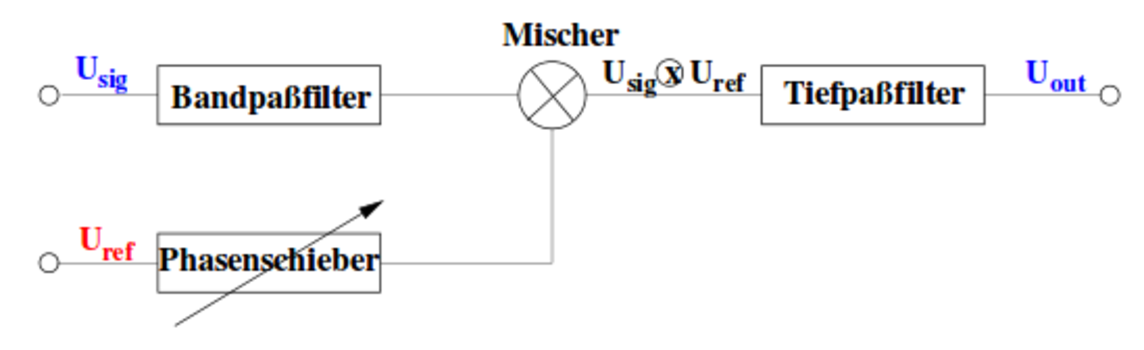
\includegraphics[width=0.7\textwidth]{Bilder/LOCK_IN.pdf}
		\caption{Schematischer Aufbau des Lock-In-Verstärkers. \cite{V303}}
		\label{fig:lockin}
	\end{figure}

Nach der Verstärkung durch den \enquote{Pre-Amplifier} durchläuft das Signal zunächst einen \enquote{Bandpassfilter}, der das Rauschen minimiert. 
Alle Frequenzen $\omega<<\omega_0$ und $\omega>>\omega_0$ werden grob herausgefiltert.
Ein \enquote{Funktionsgenerator} erzeugt die Referenzspannung $U_\mathup{ref}$ -- eine Sinus- oder Rechteckspannung der Frequenz $\omega_0$ -- , welche über den \enquote{Phasenschieber} an die Phase des Eingangssignals angepasst werden kann. 
Dieser Vorgang nennt sich Synchronisation.
Im \enquote{Mischer} treffen beide Signale aufeinander und werden multipliziert. 
Anschließend wird das Mischsignal $U_\mathup{sig}\times U_\mathup{ref}$ an den \enquote{Tiefpass} weitergeleitet, der die Modulationsfrequenz $\omega_0$ über mehrere Perioden integriert, um restliche Rauschanteile $\omega\neq\omega_0$ auszuschließen. 
Zurück bleiben nur die Anteile der Signalsspannung $U_\mathup{sig}$, die mit der Referenzspannung synchronisiert werden konnten.
Um eine möglichst geringe Bandbreite $\Delta{\nu}=\frac{1}{\pi RC}$ zu erhalten, sollte die Zeitkonstante $\uptau=RC$ des \enquote{Tiefpasses} ausreichend groß gewählt werden. 
Damit wird eine hohe Güteziffer im Bezug auf Störungsfilterung erzielt.

Die Ausgangsspannung $U_\mathup{out}$ ist eine Gleichspannung, welche proportional zur Eingangsspannung $U_\mathup{sig}$ und zum Cosinus der Phasendifferenz $\Delta\Phi$ ist:
\begin{equation}
 	U_\mathup{out}\propto{U_\text{sig}}\text{cos}(\Delta\Phi). 
 	\label{cosinus_ausgangsspannung}
 \end{equation} 
$U_\mathup{out}$ wird also maximal, wenn die Phasendifferenz $\Delta\Phi=0$ (wahlweise Vielfache von 180°) beträgt. \cite{regensburg}
%Quellenangabe http://www.physik.uni-regensburg.de/studium/praktika/a2/download/versuch5a.pdf

\begin{figure}
	\centering
		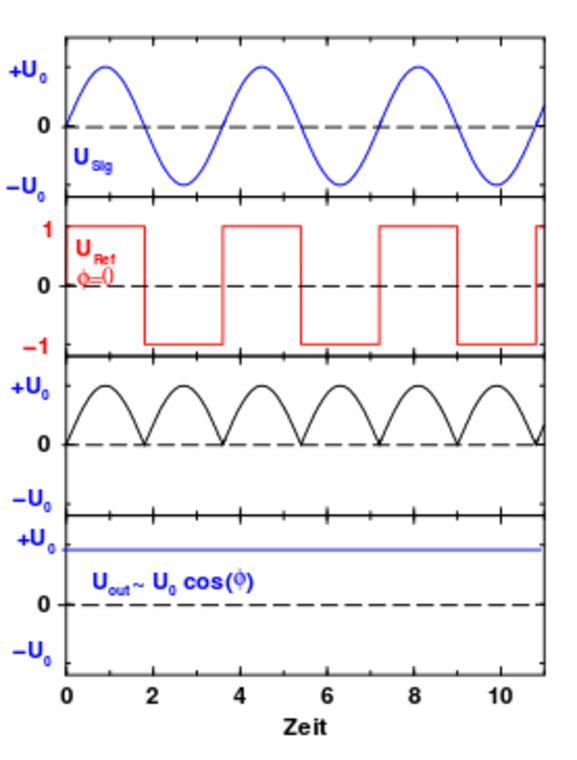
\includegraphics[width=0.4\textwidth]{Bilder/Beispiel.pdf}
		\caption{Überlagerung eines sinusförmigen Eingangssignals mit rechteckiger Referenzsspannung. \cite{V303}}
		\label{fig:bsp}
	\end{figure}
Wird beispielsweise ein sinusförmiges Eingangssignal $U_\mathup{sig}=U_0sin(\omega t)$ wie in Abbildug \ref{fig:bsp} mit einem rechteckigen Referenzsignal $U_\mathup{ref}$ gleicher Frequenz überlagert, wird diese zunächst durch eine Fourierreihe angenähert, welche aus den ungeraden Harmonischen der Grundfrequenz besteht. 
Wird das multiplizierte Signal,  bestehend aus geraden Oberwellen der Frequenz $\omega$ durch den als Gleichrichter funktionierenden Tiefpass geleitet ergibt sich die Gleichspannung
\begin{equation}
	U_\mathup{out}=\frac{2}{\pi}U_0\text{cos}(\Phi).
\end{equation}
Besteht kein Phasenunterschied zwischen Eingangs- und Referenzsignal nimmt die Ausgangsspannung ihren Maximalwert 
\begin{equation}
	U_\mathup{out}=\frac{2}{\pi}U_0
\end{equation}
an.
Die Rechteckspannung mit auf 1 genormter Amplitude realisiert einen Schalter (\enquote{Chopper}). 
Indem die Werte 1 und -1 durch positive und negative Halbwellen angenommen werden, steht der Schalter auf \enquote{Ein} bzw. \enquote{Aus}.




\section{Durchführung}
\label{sec:Durchfuehrung}
\subsection{Freie Schwingung mit Dämpfung}
Im ersten Teil wird die freie, gedämpfte Schwingung mit einem Serienschwingkreis untersucht.
Es wird die Zeitabhängigkeit der Kondensatorspannung $U_\mathup{C}(\omega, t)$ betrachtet und ihr Verlauf diskutiert.
Hierzu wird eine Schaltung wie in Abbildung \ref{fig:schaltkreis_erzwungen} angesetzt.
Der Generator wird auf Rechteckspannung mit einer solch geringen Frequenz $f$ eingestellt, dass innerhalb einer Periode des Generator das System frei oszillieren und abklingen kann, ehe es nach der Periodendauer $\frac{1}{f}$ erneut angeregt wird.
Die weiteren Systemparameter, etwa die Komponenten des Schwingkreises, werden so gewählt, dass die charakteristischen Verläufe sichtbar werden. 
Die Verläufe der Kondensatorspannung $U_\mathup{C}(\omega, t)$ werden dargestellt und gespeichert.

Die systembeschreibende Abklingzeit $T_\text{ex}$ wird an diesen Verläufen bestimmt und mit dem vorhergesagten Wert nach der Gleichung \eqref{eq:abkling} verglichen.\\
Der aperiodische Grenzfall wird als Grenze zwischen Kriechfall und Schwingfall mittels Bisektion des Dämpfungswiderstandes $R$ angenähert, wozu der Schwingkreis mit einem variablen Widerstand ausgestattet wird.
Der auf diese Weise ermittelte Dämpfungswiderstand $R_\text{ap}$ wird mit dem theoretischen Wert $R_\text{ap,t}$ aus \ref{sec:theorie1} verglichen.

\subsection{Erzwungene Schwingung mit Dämpfung}
Im zweiten Teil wird die erzwungene, gedämpfte Schwingung untersucht.
Gemessen wird die Frequenzabhängigkeit der Kondensatorspannung $U_\mathup{C}(\omega, t)$ eines Serienschwingkreises sowie der Phasenwinkel $\phi$ zwischen der Erregerspannung $U(t)$ und der Kondensatorspannung $U_\mathup{C}(\omega, t)$.\\
Hierzu wird einerseits bei verschiedenen Erregerfrequenzen $U(t)$  der Betrag der Kondensatorspannung $U_\mathup{C}(\omega, t)$ und die Zeitdifferenz der Nulldurchgänge von Erregerspannung $U(t)$ und von der Kondensatorspannung $U_\mathup{C}(\omega, t)$ betrachtet.
Weiter wird zur Charakterisierung des Resonanzverhaltens die Güte $q$ und die Resonanzbreite $\mathup{\Delta}\, f$ bestimmt.

% Ein Wanderurlaub im ehemaligen Jugoslawien. Klingt zunächst einmal furchtbar spannend, ist aber eigentlich der Gähner (=Langeweiler, langweilige Sache) überhaupt.

% Jeder denkt: Alte Militärbaracken, Herrenausstatter wohin man schaut, vielleicht ein Museum für altertümliche Fahrstuhltechnik, klingt doch toll! Doch hält diese vorgefasste Meinung einer genaueren Betrachtung nicht stand. Schon morgens im Hotel wird die Kehrseite der Medaille deutlich:

% Aufzug defekt. Buffet unvollständig. Chinesische Loungemusik. Despotisches Hotelpersonal. Eierlikör ausverkauft. Französischer Kofferträger. Gewaltsamer Raubüberfall. Hasenzähnige Empfangsdame. Interplanetarer Schmugglerstützpunkt. Jodelmusikkorps nebenan. Kreditkarte gesperrt. Lilafarbener Teppichläufer. Monochromatisches Licht. Nucleophile Substitution. Ortsunkundige Japaner. Präsidentenleiche unübersehbar. Qualmender Ethanolofen. Resistiver Touchscreen. Systematische Tötungen. Trauriger Clown. Unerfreuliche Massenbegräbnisse. Verwanzte Matratzen. Wadenkrampffördernde Beleuchtung. X-Beinige Pianodame. Yorkshireterrier bellt. Bezahlung nur bar möglich (und nicht per EC-Karte, wie ich es sonst immer mache).

% Also merke: Der Spruch „Im Norden geht die Sonne auf, im Süden nimmt sie Ihren Lauf, […] Westen wird sie untergehen, usw.“, gilt nicht wenn man auf dem Mond (oder einem anderen Erdtrabanten) steht (oder sitzt, außer man liegt).

\section{Auswertung}
\label{sec:Auswertung}
\begin{table}
	\centering
	\begin{tabular}{S[table-format=2.0] S[table-format=3.0] S[table-format=3.0] S[table-format=2.2]}
	\toprule
{$n$} & {$U_n/\:\si{\milli{\volt}}$} & {$\frac{U_1}{n}/\:\si{\milli{\volt}}$} & {Abweichung in $\%$}\\
	\midrule
 1 & 920 & 912 &  1\\
 3 & 300 & 288 &  4\\
 5 & 170 & 168 &  1\\
 7 & 116 & 112 &  4\\
 9 &  86 &  80 &  8\\
11 &  64 &  56 & 14\\
	\bottomrule
	\end{tabular}
	\caption{Fourieranalyse der Rechteckspannung.}
	\label{tab:FA_RE}
\end{table}
 
\begin{table}
	\centering
	\sisetup{table-format=2.3}
	\begin{tabular}{S[table-format=2.0] S[table-format=3.0] S[table-format=3.1] S[table-format=1.2] }
	\toprule
	{$n$} & {$U_n/\:\si{\milli\volt}$} & {$\frac{U_1}{n}/\:\si{\milli\volt}$} & {Abweichung in $\%$}\\
	\midrule
 1 & 580 & 576.0 & 0.7\\
 3 &  63 &  61.6 & 2.3\\
 5 &  21 &  20.8 & 1.0\\
 7 &  10 &  10.4 & 3.9\\
 9 &   6 &   5.6 & 7.1\\
11 &   4 &   4.0 & 0.0\\
	\bottomrule
	\end{tabular}
	\caption{Fourieranalyse der Dreiecksspannung.}
	\label{tab:FA_RE}
\end{table}



\begin{table}
	\centering
	\sisetup{table-format=2.3}
	\begin{tabular}{S[table-format=2.0] S[table-format=3.0] S[table-format=3.1] S[table-format=1.0] }
	\toprule
	{$n$} & {$U_n/\:\si{\milli\volt}$} & {$\frac{U_1}{n}/\:\si{\milli\volt}$} & {Abweichung in $\%$}\\
	\midrule
 1 & 460 & 456 & 1\\
 2 & 230 & 224 & 3\\
 3 & 152 & 144 & 6\\
 4 & 112 & 112 & 0\\
 5 &  88 &  88 & 0\\
 6 &  74 &  74 & 0\\
 7 &  64 &  64 & 0\\
 8 &  56 &  56 & 0\\
 9 &  50 &  48 & 4\\
10 &  44 &  46 & 5\\
11 &  40 &  40 & 0\\
	\bottomrule
	\end{tabular}
	\caption{Fourieranalyse der Sägezahnspannung.}
	\label{tab:FA_RE}
\end{table}



\section{Diskussion}
\label{sec:Diskussion}

\subsection{Fehlerdiskussion}
Für die Fehlerdiskussion verwertbare Messwerte wurden in Abschnitt \ref{sec:Auswertung2}, Tabelle \ref{tab:block_messung} sowie in Abschnitt \ref{sec:Auswertung3}, Tabelle \ref{tab:auge} beschrieben.
Für die Bestimmung dieser Messwerte wurde der Betrag der Schallgeschwindigkeit in Abschnitt \ref{sec:Auswertung1}, Gleichung \eqref{qu:geschwindigkeit} gefunden.
Die geringe Abweichung von dem Literaturwert bezeugt, dass es nicht zu systematischen Fehlern kam und das Grundprinzip der Messung ein zuverlässiges Ergebnis liefert.

Die starken Abweichungen bei der Bestimmung der Materialfehler $a$ im Block von bis zu $27\%$ und 
bei der Bestimmung des Lochdurchmessers $d$ von bis zu $233\%$.
Die starke Abweichung in der Unsicherheit im Laufe der Messung weist auf starke statistische Fehler und eine ungeeignete Wahl der Schallfrequenz hin. 
Die Maßstäbe des Augenmodells, das als brauchbares $1$:$3$-Modell angenommen wird, wurden mit starker Abweichung von der Literaturangabe bestimmt.
Dies weist ähnlich zum vorangegangen Fall auf ungeeignete Wahl der Frequenz hin.

\subsection{Verwendung des Ultraschall-Verfahrens}
Es konnte im Experiment die Anwendbarkeit des Ultraschall-Verfahrens zur Feststellung von Materialfehlern und, bei geeignetem Aufbau sowie geeigneter Wahl der Einstellungen, die Tiefenauflösung nachgewiesen werden.
Das Prinzip ist somit in Industrie zur zerstörungsfreien Fehlerprüfung und in der Medizin zur nicht-invasiven Maßnahme als bildgebendes Verfahren verwendbar.
%\section{Daten}
%\begin{longtable}{rrllllllll}%[htbp]
	\hline
	{ID}&{Zeit/\si{\second}} &{$\theta_{1}$/\si{\degreeCelsius}}&{$\theta_{2}$/\si{\degreeCelsius}}&{$\theta_{3}$/\si{\degreeCelsius}}&{$\theta_{4}$/\si{\degreeCelsius}}&{$\theta_{5}$/\si{\degreeCelsius}}&{$\theta_{6}$/\si{\degreeCelsius}}&{$\theta_{7}$/\si{\degreeCelsius}}&{$\theta_{8}$/\si{\degreeCelsius}}\\
	\hline
	\endhead
1 & 0 & 21.85 & 23.61 & 23.12 & 21.43 & 22.36 & 23.60 & 22.24 & 20.82 \\ 
2 & 5 & 22.07 & 24.07 & 23.59 & 21.64 & 22.73 & 24.04 & 22.68 & 20.83 \\ 
3 & 10 & 22.30 & 24.48 & 24.01 & 21.87 & 23.10 & 24.44 & 23.12 & 20.84 \\ 
4 & 15 & 22.53 & 24.85 & 24.39 & 22.11 & 23.46 & 24.81 & 23.55 & 20.86 \\ 
5 & 20 & 22.76 & 25.18 & 24.73 & 22.34 & 23.82 & 25.16 & 23.95 & 20.90 \\ 
6 & 25 & 23.00 & 25.49 & 25.03 & 22.59 & 24.17 & 25.47 & 24.33 & 20.95 \\ 
7 & 30 & 23.23 & 25.77 & 25.32 & 22.82 & 24.50 & 25.78 & 24.68 & 20.98 \\ 
8 & 35 & 23.46 & 26.02 & 25.58 & 23.04 & 24.83 & 26.06 & 25.02 & 21.04 \\ 
9 & 40 & 23.69 & 26.27 & 25.82 & 23.27 & 25.14 & 26.33 & 25.33 & 21.10 \\ 
10 & 45 & 23.91 & 26.50 & 26.04 & 23.48 & 25.44 & 26.59 & 25.62 & 21.17 \\ 
11 & 50 & 24.12 & 26.71 & 26.25 & 23.69 & 25.72 & 26.83 & 25.88 & 21.23 \\ 
12 & 55 & 24.33 & 26.93 & 26.46 & 23.90 & 26.00 & 27.07 & 26.14 & 21.32 \\ 
13 & 60 & 24.54 & 27.13 & 26.65 & 24.10 & 26.26 & 27.29 & 26.37 & 21.40 \\ 
14 & 65 & 24.75 & 27.32 & 26.83 & 24.30 & 26.53 & 27.50 & 26.59 & 21.48 \\ 
15 & 70 & 24.94 & 27.50 & 27.00 & 24.48 & 26.76 & 27.71 & 26.80 & 21.56 \\ 
16 & 75 & 25.13 & 27.67 & 27.16 & 24.67 & 26.99 & 27.91 & 27.00 & 21.65 \\ 
17 & 80 & 25.33 & 27.85 & 27.33 & 24.85 & 27.23 & 28.11 & 27.19 & 21.74 \\ 
18 & 85 & 25.51 & 28.01 & 27.47 & 25.02 & 27.44 & 28.28 & 27.37 & 21.83 \\ 
19 & 90 & 25.68 & 28.17 & 27.62 & 25.19 & 27.64 & 28.46 & 27.54 & 21.93 \\ 
20 & 95 & 25.86 & 28.32 & 27.76 & 25.36 & 27.85 & 28.62 & 27.70 & 22.01 \\ 
21 & 100 & 26.03 & 28.47 & 27.89 & 25.52 & 28.04 & 28.79 & 27.85 & 22.10 \\ 
22 & 105 & 26.20 & 28.61 & 28.01 & 25.65 & 28.22 & 28.94 & 27.99 & 22.19 \\ 
23 & 110 & 26.36 & 28.76 & 28.14 & 25.81 & 28.40 & 29.10 & 28.13 & 22.28 \\ 
24 & 115 & 26.52 & 28.89 & 28.27 & 25.96 & 28.57 & 29.24 & 28.26 & 22.37 \\ 
25 & 120 & 26.67 & 29.02 & 28.39 & 26.11 & 28.73 & 29.38 & 28.39 & 22.46 \\ 
26 & 125 & 26.82 & 29.15 & 28.51 & 26.25 & 28.89 & 29.52 & 28.52 & 22.55 \\ 
27 & 130 & 26.97 & 29.28 & 28.62 & 26.37 & 29.05 & 29.64 & 28.64 & 22.64 \\ 
28 & 135 & 27.12 & 29.40 & 28.73 & 26.50 & 29.19 & 29.77 & 28.75 & 22.72 \\ 
29 & 140 & 27.26 & 29.52 & 28.84 & 26.64 & 29.34 & 29.90 & 28.86 & 22.81 \\ 
30 & 145 & 27.40 & 29.64 & 28.95 & 26.75 & 29.48 & 30.02 & 28.97 & 22.89 \\ 
31 & 150 & 27.53 & 29.76 & 29.05 & 26.88 & 29.61 & 30.13 & 29.07 & 22.98 \\ 
32 & 155 & 27.66 & 29.87 & 29.15 & 26.99 & 29.74 & 30.25 & 29.18 & 23.06 \\ 
33 & 160 & 27.79 & 29.99 & 29.26 & 27.11 & 29.87 & 30.36 & 29.28 & 23.14 \\ 
34 & 165 & 27.92 & 30.10 & 29.35 & 27.23 & 29.99 & 30.47 & 29.38 & 23.23 \\ 
35 & 170 & 28.04 & 30.20 & 29.45 & 27.34 & 30.11 & 30.58 & 29.47 & 23.30 \\ 
36 & 175 & 28.16 & 30.31 & 29.55 & 27.45 & 30.23 & 30.68 & 29.56 & 23.39 \\ 
37 & 180 & 28.28 & 30.42 & 29.64 & 27.55 & 30.34 & 30.79 & 29.65 & 23.46 \\ 
38 & 185 & 28.40 & 30.53 & 29.73 & 27.66 & 30.45 & 30.89 & 29.74 & 23.54 \\ 
39 & 190 & 28.52 & 30.63 & 29.83 & 27.76 & 30.56 & 30.98 & 29.83 & 23.62 \\ 
40 & 195 & 28.63 & 30.73 & 29.91 & 27.86 & 30.68 & 31.08 & 29.91 & 23.70 \\ 
41 & 200 & 28.74 & 30.83 & 30.01 & 27.96 & 30.78 & 31.17 & 30.00 & 23.77 \\ 
42 & 205 & 28.85 & 30.92 & 30.09 & 28.06 & 30.88 & 31.27 & 30.08 & 23.85 \\ 
43 & 210 & 28.96 & 31.02 & 30.18 & 28.15 & 30.98 & 31.36 & 30.17 & 23.92 \\ 
44 & 215 & 29.06 & 31.11 & 30.26 & 28.24 & 31.08 & 31.44 & 30.24 & 24.00 \\ 
45 & 220 & 29.17 & 31.21 & 30.35 & 28.33 & 31.17 & 31.53 & 30.31 & 24.06 \\ 
46 & 225 & 29.27 & 31.30 & 30.43 & 28.43 & 31.27 & 31.62 & 30.39 & 24.14 \\ 
47 & 230 & 29.37 & 31.40 & 30.52 & 28.52 & 31.36 & 31.71 & 30.48 & 24.21 \\ 
48 & 235 & 29.48 & 31.49 & 30.59 & 28.60 & 31.45 & 31.79 & 30.55 & 24.27 \\ 
49 & 240 & 29.57 & 31.58 & 30.68 & 28.69 & 31.54 & 31.88 & 30.63 & 24.35 \\ 
50 & 245 & 29.67 & 31.66 & 30.76 & 28.78 & 31.63 & 31.96 & 30.70 & 24.42 \\ 
51 & 250 & 29.76 & 31.75 & 30.83 & 28.87 & 31.72 & 32.04 & 30.77 & 24.49 \\ 
52 & 255 & 29.85 & 31.84 & 30.91 & 28.94 & 31.80 & 32.12 & 30.85 & 24.57 \\ 
53 & 260 & 29.95 & 31.92 & 30.99 & 29.02 & 31.89 & 32.20 & 30.92 & 24.63 \\ 
54 & 265 & 30.03 & 32.00 & 31.07 & 29.11 & 31.97 & 32.28 & 30.99 & 24.70 \\ 
55 & 270 & 30.12 & 32.08 & 31.14 & 29.19 & 32.05 & 32.35 & 31.06 & 24.77 \\ 
56 & 275 & 30.22 & 32.16 & 31.21 & 29.27 & 32.13 & 32.43 & 31.13 & 24.83 \\ 
57 & 280 & 30.29 & 32.25 & 31.29 & 29.34 & 32.21 & 32.51 & 31.19 & 24.89 \\ 
58 & 285 & 30.39 & 32.34 & 31.37 & 29.42 & 32.29 & 32.59 & 31.26 & 24.96 \\ 
59 & 290 & 30.47 & 32.42 & 31.44 & 29.50 & 32.37 & 32.66 & 31.33 & 25.02 \\ 
60 & 295 & 30.56 & 32.49 & 31.51 & 29.58 & 32.45 & 32.73 & 31.40 & 25.08 \\ 
61 & 300 & 30.64 & 32.57 & 31.58 & 29.65 & 32.53 & 32.80 & 31.47 & 25.15 \\ 
62 & 305 & 30.72 & 32.64 & 31.65 & 29.72 & 32.60 & 32.87 & 31.53 & 25.22 \\ 
63 & 310 & 30.80 & 32.73 & 31.73 & 29.80 & 32.67 & 32.95 & 31.60 & 25.27 \\ 
64 & 315 & 30.89 & 32.82 & 31.81 & 29.87 & 32.75 & 33.02 & 31.67 & 25.34 \\ 
65 & 320 & 30.96 & 32.90 & 31.88 & 29.94 & 32.81 & 33.10 & 31.72 & 25.39 \\ 
66 & 325 & 31.04 & 32.99 & 31.97 & 30.01 & 32.89 & 33.17 & 31.81 & 25.46 \\ 
67 & 330 & 31.13 & 33.08 & 32.05 & 30.10 & 32.98 & 33.25 & 31.87 & 25.52 \\ 
68 & 335 & 31.21 & 33.15 & 32.12 & 30.17 & 33.06 & 33.33 & 31.94 & 25.59 \\ 
69 & 340 & 31.29 & 33.23 & 32.19 & 30.24 & 33.13 & 33.40 & 32.01 & 25.65 \\ 
70 & 345 & 31.37 & 33.31 & 32.26 & 30.32 & 33.21 & 33.48 & 32.08 & 25.71 \\ 
71 & 350 & 31.46 & 33.39 & 32.33 & 30.40 & 33.29 & 33.55 & 32.14 & 25.77 \\ 
72 & 355 & 31.53 & 33.46 & 32.40 & 30.46 & 33.37 & 33.62 & 32.21 & 25.83 \\ 
73 & 360 & 31.62 & 33.54 & 32.47 & 30.53 & 33.44 & 33.70 & 32.28 & 25.89 \\ 
74 & 365 & 31.69 & 33.61 & 32.53 & 30.60 & 33.52 & 33.77 & 32.34 & 25.95 \\ 
75 & 370 & 31.77 & 33.69 & 32.60 & 30.67 & 33.59 & 33.84 & 32.40 & 26.01 \\ 
76 & 375 & 31.85 & 33.76 & 32.67 & 30.73 & 33.66 & 33.91 & 32.46 & 26.07 \\ 
77 & 380 & 31.92 & 33.84 & 32.73 & 30.80 & 33.74 & 33.98 & 32.53 & 26.13 \\ 
78 & 385 & 32.00 & 33.91 & 32.80 & 30.87 & 33.81 & 34.05 & 32.58 & 26.19 \\ 
79 & 390 & 32.07 & 33.98 & 32.86 & 30.93 & 33.88 & 34.12 & 32.64 & 26.25 \\ 
80 & 395 & 32.15 & 34.05 & 32.92 & 31.00 & 33.95 & 34.18 & 32.71 & 26.31 \\ 
81 & 400 & 32.21 & 34.12 & 32.98 & 31.06 & 34.02 & 34.25 & 32.76 & 26.36 \\ 
82 & 405 & 32.29 & 34.18 & 33.05 & 31.13 & 34.08 & 34.31 & 32.82 & 26.42 \\ 
83 & 410 & 32.36 & 34.25 & 33.11 & 31.18 & 34.15 & 34.38 & 32.88 & 26.48 \\ 
84 & 415 & 32.43 & 34.32 & 33.17 & 31.25 & 34.22 & 34.44 & 32.94 & 26.54 \\ 
85 & 420 & 32.50 & 34.39 & 33.23 & 31.31 & 34.29 & 34.51 & 33.00 & 26.59 \\ 
86 & 425 & 32.57 & 34.45 & 33.29 & 31.38 & 34.35 & 34.57 & 33.06 & 26.65 \\ 
87 & 430 & 32.63 & 34.52 & 33.35 & 31.44 & 34.42 & 34.63 & 33.12 & 26.70 \\ 
88 & 435 & 32.70 & 34.58 & 33.41 & 31.50 & 34.48 & 34.69 & 33.17 & 26.76 \\ 
89 & 440 & 32.76 & 34.64 & 33.47 & 31.56 & 34.54 & 34.75 & 33.23 & 26.81 \\ 
90 & 445 & 32.83 & 34.71 & 33.53 & 31.62 & 34.60 & 34.81 & 33.28 & 26.87 \\ 
91 & 450 & 32.89 & 34.77 & 33.58 & 31.68 & 34.67 & 34.87 & 33.34 & 26.93 \\ 
92 & 455 & 32.96 & 34.83 & 33.64 & 31.73 & 34.73 & 34.93 & 33.39 & 26.98 \\ 
93 & 460 & 33.02 & 34.89 & 33.70 & 31.78 & 34.79 & 34.99 & 33.44 & 27.03 \\ 
94 & 465 & 33.08 & 34.95 & 33.76 & 31.85 & 34.85 & 35.05 & 33.50 & 27.09 \\ 
95 & 470 & 33.14 & 35.01 & 33.81 & 31.90 & 34.91 & 35.10 & 33.55 & 27.14 \\ 
96 & 475 & 33.21 & 35.07 & 33.86 & 31.96 & 34.96 & 35.16 & 33.60 & 27.19 \\ 
97 & 480 & 33.27 & 35.13 & 33.92 & 32.01 & 35.02 & 35.21 & 33.66 & 27.24 \\ 
98 & 485 & 33.33 & 35.19 & 33.97 & 32.07 & 35.07 & 35.27 & 33.71 & 27.30 \\ 
99 & 490 & 33.39 & 35.25 & 34.03 & 32.12 & 35.13 & 35.32 & 33.76 & 27.35 \\ 
100 & 495 & 33.45 & 35.30 & 34.08 & 32.17 & 35.19 & 35.38 & 33.82 & 27.40 \\ 
101 & 500 & 33.51 & 35.36 & 34.13 & 32.23 & 35.25 & 35.43 & 33.86 & 27.45 \\ 
102 & 505 & 33.56 & 35.42 & 34.18 & 32.28 & 35.30 & 35.48 & 33.91 & 27.50 \\ 
103 & 510 & 33.62 & 35.47 & 34.23 & 32.33 & 35.35 & 35.54 & 33.96 & 27.55 \\ 
104 & 515 & 33.68 & 35.53 & 34.28 & 32.39 & 35.41 & 35.58 & 34.01 & 27.60 \\ 
105 & 520 & 33.73 & 35.58 & 34.33 & 32.44 & 35.46 & 35.63 & 34.06 & 27.65 \\ 
106 & 525 & 33.79 & 35.63 & 34.38 & 32.49 & 35.51 & 35.69 & 34.11 & 27.70 \\ 
107 & 530 & 33.85 & 35.69 & 34.43 & 32.54 & 35.56 & 35.73 & 34.16 & 27.75 \\ 
108 & 535 & 33.90 & 35.74 & 34.48 & 32.59 & 35.62 & 35.79 & 34.20 & 27.80 \\ 
109 & 540 & 33.95 & 35.79 & 34.53 & 32.65 & 35.66 & 35.83 & 34.25 & 27.85 \\ 
110 & 545 & 34.01 & 35.84 & 34.58 & 32.69 & 35.72 & 35.88 & 34.30 & 27.90 \\ 
111 & 550 & 34.06 & 35.90 & 34.63 & 32.74 & 35.76 & 35.94 & 34.35 & 27.95 \\ 
112 & 555 & 34.11 & 35.95 & 34.68 & 32.78 & 35.81 & 35.98 & 34.39 & 28.00 \\ 
113 & 560 & 34.16 & 36.00 & 34.72 & 32.83 & 35.86 & 36.03 & 34.44 & 28.05 \\ 
114 & 565 & 34.21 & 36.05 & 34.77 & 32.88 & 35.91 & 36.07 & 34.49 & 28.08 \\ 
115 & 570 & 34.27 & 36.10 & 34.82 & 32.93 & 35.96 & 36.12 & 34.53 & 28.13 \\ 
116 & 575 & 34.32 & 36.15 & 34.87 & 32.98 & 36.01 & 36.17 & 34.58 & 28.18 \\ 
117 & 580 & 34.37 & 36.20 & 34.91 & 33.02 & 36.05 & 36.22 & 34.62 & 28.22 \\ 
118 & 585 & 34.42 & 36.24 & 34.96 & 33.07 & 36.10 & 36.26 & 34.67 & 28.27 \\ 
119 & 590 & 34.46 & 36.30 & 35.01 & 33.11 & 36.15 & 36.31 & 34.72 & 28.32 \\ 
120 & 595 & 34.51 & 36.35 & 35.05 & 33.16 & 36.19 & 36.36 & 34.77 & 28.37 \\ 
121 & 600 & 34.57 & 36.40 & 35.10 & 33.21 & 36.24 & 36.40 & 34.81 & 28.41 \\ 
122 & 605 & 34.61 & 36.45 & 35.14 & 33.25 & 36.29 & 36.45 & 34.86 & 28.46 \\ 
123 & 610 & 34.66 & 36.49 & 35.19 & 33.30 & 36.34 & 36.49 & 34.90 & 28.50 \\ 
124 & 615 & 34.71 & 36.54 & 35.23 & 33.35 & 36.38 & 36.54 & 34.94 & 28.55 \\ 
125 & 620 & 34.76 & 36.59 & 35.28 & 33.39 & 36.42 & 36.58 & 34.99 & 28.59 \\ 
126 & 625 & 34.81 & 36.63 & 35.33 & 33.44 & 36.47 & 36.63 & 35.03 & 28.64 \\ 
127 & 630 & 34.85 & 36.68 & 35.37 & 33.48 & 36.52 & 36.67 & 35.08 & 28.69 \\ 
128 & 635 & 34.90 & 36.72 & 35.41 & 33.53 & 36.56 & 36.72 & 35.12 & 28.73 \\ 
129 & 640 & 34.95 & 36.77 & 35.45 & 33.57 & 36.60 & 36.76 & 35.17 & 28.77 \\ 
130 & 645 & 34.99 & 36.81 & 35.50 & 33.61 & 36.65 & 36.80 & 35.21 & 28.82 \\ 
131 & 650 & 35.04 & 36.87 & 35.55 & 33.66 & 36.69 & 36.85 & 35.25 & 28.86 \\ 
132 & 655 & 35.08 & 36.91 & 35.59 & 33.70 & 36.74 & 36.89 & 35.29 & 28.91 \\ 
133 & 660 & 35.13 & 36.95 & 35.63 & 33.74 & 36.78 & 36.93 & 35.33 & 28.95 \\ 
134 & 665 & 35.17 & 37.00 & 35.67 & 33.79 & 36.82 & 36.98 & 35.38 & 28.99 \\ 
135 & 670 & 35.22 & 37.05 & 35.71 & 33.83 & 36.86 & 37.02 & 35.42 & 29.03 \\ 
136 & 675 & 35.25 & 37.09 & 35.76 & 33.88 & 36.91 & 37.07 & 35.46 & 29.07 \\ 
137 & 680 & 35.30 & 37.13 & 35.80 & 33.91 & 36.95 & 37.10 & 35.50 & 29.12 \\ 
138 & 685 & 35.35 & 37.17 & 35.84 & 33.96 & 36.99 & 37.15 & 35.55 & 29.16 \\ 
139 & 690 & 35.39 & 37.22 & 35.88 & 33.99 & 37.04 & 37.19 & 35.59 & 29.20 \\ 
140 & 695 & 35.43 & 37.26 & 35.92 & 34.04 & 37.08 & 37.23 & 35.63 & 29.24 \\ 
141 & 700 & 35.48 & 37.30 & 35.96 & 34.08 & 37.12 & 37.27 & 35.67 & 29.28 \\ 
142 & 705 & 35.52 & 37.34 & 36.01 & 34.12 & 37.16 & 37.31 & 35.71 & 29.32 \\ 
143 & 710 & 35.56 & 37.39 & 36.05 & 34.16 & 37.20 & 37.35 & 35.75 & 29.37 \\ 
144 & 715 & 35.60 & 37.43 & 36.09 & 34.20 & 37.24 & 37.39 & 35.79 & 29.41 \\ 
145 & 720 & 35.64 & 37.48 & 36.13 & 34.24 & 37.28 & 37.44 & 35.83 & 29.45 \\ 
146 & 725 & 35.69 & 37.52 & 36.17 & 34.28 & 37.32 & 37.47 & 35.87 & 29.49 \\ 
147 & 730 & 35.72 & 37.56 & 36.21 & 34.32 & 37.36 & 37.51 & 35.91 & 29.54 \\ 
148 & 735 & 35.77 & 37.60 & 36.25 & 34.35 & 37.40 & 37.55 & 35.95 & 29.57 \\ 
149 & 740 & 35.81 & 37.64 & 36.29 & 34.39 & 37.44 & 37.59 & 35.99 & 29.61 \\ 
150 & 745 & 35.85 & 37.68 & 36.33 & 34.44 & 37.47 & 37.63 & 36.03 & 29.65 \\ 
151 & 750 & 35.89 & 37.72 & 36.37 & 34.48 & 37.52 & 37.67 & 36.07 & 29.69 \\ 
152 & 755 & 35.93 & 37.77 & 36.41 & 34.52 & 37.55 & 37.71 & 36.11 & 29.73 \\ 
153 & 760 & 35.96 & 37.80 & 36.44 & 34.55 & 37.59 & 37.75 & 36.15 & 29.77 \\ 
154 & 765 & 36.01 & 37.85 & 36.48 & 34.59 & 37.63 & 37.79 & 36.19 & 29.81 \\ 
155 & 770 & 36.05 & 37.89 & 36.52 & 34.62 & 37.66 & 37.82 & 36.22 & 29.84 \\ 
156 & 775 & 36.08 & 37.92 & 36.55 & 34.65 & 37.70 & 37.85 & 36.24 & 29.87 \\ 
157 & 780 & 36.12 & 37.97 & 36.60 & 34.70 & 37.74 & 37.90 & 36.30 & 29.92 \\ 
158 & 785 & 36.15 & 37.99 & 36.63 & 34.74 & 37.76 & 37.91 & 36.34 & 29.96 \\ 
159 & 790 & 36.20 & 38.04 & 36.67 & 34.78 & 37.81 & 37.96 & 36.38 & 30.00 \\ 
160 & 795 & 36.24 & 38.09 & 36.70 & 34.80 & 37.84 & 38.00 & 36.41 & 30.04 \\ 
161 & 800 & 36.27 & 38.12 & 36.74 & 34.85 & 37.88 & 38.05 & 36.46 & 30.08 \\ 
162 & 805 & 36.31 & 38.15 & 36.78 & 34.88 & 37.92 & 38.08 & 36.49 & 30.11 \\ 
163 & 810 & 36.34 & 38.19 & 36.82 & 34.92 & 37.95 & 38.12 & 36.53 & 30.15 \\ 
164 & 815 & 36.38 & 38.23 & 36.86 & 34.96 & 37.98 & 38.15 & 36.57 & 30.19 \\ 
165 & 820 & 36.41 & 38.27 & 36.90 & 35.00 & 38.03 & 38.19 & 36.61 & 30.23 \\ 
166 & 825 & 36.45 & 38.31 & 36.93 & 35.03 & 38.06 & 38.23 & 36.65 & 30.27 \\ 
167 & 830 & 36.49 & 38.34 & 36.97 & 35.06 & 38.09 & 38.26 & 36.69 & 30.30 \\ 
168 & 835 & 36.52 & 38.38 & 37.00 & 35.10 & 38.13 & 38.30 & 36.72 & 30.34 \\ 
169 & 840 & 36.56 & 38.42 & 37.04 & 35.13 & 38.16 & 38.33 & 36.76 & 30.38 \\ 
170 & 845 & 36.60 & 38.46 & 37.08 & 35.17 & 38.20 & 38.36 & 36.80 & 30.42 \\ 
171 & 850 & 36.64 & 38.50 & 37.12 & 35.21 & 38.24 & 38.40 & 36.84 & 30.45 \\ 
172 & 855 & 36.67 & 38.53 & 37.15 & 35.24 & 38.28 & 38.44 & 36.87 & 30.49 \\ 
173 & 860 & 36.71 & 38.57 & 37.18 & 35.28 & 38.31 & 38.48 & 36.91 & 30.52 \\ 
174 & 865 & 36.74 & 38.61 & 37.22 & 35.31 & 38.35 & 38.52 & 36.94 & 30.55 \\ 
175 & 870 & 36.78 & 38.65 & 37.24 & 35.32 & 38.39 & 38.56 & 36.96 & 30.57 \\ 
176 & 875 & 36.81 & 38.68 & 37.28 & 35.37 & 38.43 & 38.59 & 37.01 & 30.62 \\ 
177 & 880 & 36.85 & 38.72 & 37.32 & 35.41 & 38.47 & 38.63 & 37.05 & 30.67 \\ 
178 & 885 & 36.89 & 38.75 & 37.36 & 35.45 & 38.50 & 38.67 & 37.09 & 30.70 \\ 
179 & 890 & 36.92 & 38.79 & 37.39 & 35.48 & 38.54 & 38.70 & 37.13 & 30.74 \\ 
180 & 895 & 36.95 & 38.82 & 37.42 & 35.51 & 38.58 & 38.74 & 37.16 & 30.77 \\ 
181 & 900 & 36.99 & 38.86 & 37.46 & 35.55 & 38.61 & 38.78 & 37.20 & 30.81 \\ 
182 & 905 & 37.02 & 38.89 & 37.50 & 35.58 & 38.65 & 38.82 & 37.24 & 30.84 \\ 
183 & 910 & 37.06 & 38.93 & 37.53 & 35.62 & 38.68 & 38.85 & 37.27 & 30.88 \\ 
184 & 915 & 37.09 & 38.96 & 37.56 & 35.65 & 38.72 & 38.88 & 37.31 & 30.92 \\ 
185 & 920 & 37.13 & 39.00 & 37.59 & 35.68 & 38.76 & 38.92 & 37.34 & 30.95 \\ 
186 & 925 & 37.16 & 39.03 & 37.63 & 35.71 & 38.79 & 38.95 & 37.38 & 30.98 \\ 
187 & 930 & 37.19 & 39.07 & 37.66 & 35.74 & 38.83 & 38.99 & 37.41 & 31.02 \\ 
188 & 935 & 37.23 & 39.10 & 37.69 & 35.76 & 38.86 & 39.02 & 37.42 & 31.03 \\ 
189 & 940 & 37.26 & 39.13 & 37.72 & 35.80 & 38.90 & 39.06 & 37.47 & 31.08 \\ 
190 & 945 & 37.30 & 39.17 & 37.76 & 35.84 & 38.93 & 39.09 & 37.52 & 31.12 \\ 
191 & 950 & 37.33 & 39.21 & 37.79 & 35.87 & 38.97 & 39.13 & 37.55 & 31.15 \\ 
192 & 955 & 37.36 & 39.24 & 37.83 & 35.91 & 39.00 & 39.16 & 37.58 & 31.19 \\ 
193 & 960 & 37.39 & 39.27 & 37.86 & 35.94 & 39.03 & 39.19 & 37.62 & 31.22 \\ 
194 & 965 & 37.43 & 39.31 & 37.89 & 35.97 & 39.07 & 39.23 & 37.65 & 31.26 \\ 
195 & 970 & 37.46 & 39.34 & 37.92 & 36.00 & 39.11 & 39.26 & 37.69 & 31.29 \\ 
196 & 975 & 37.50 & 39.37 & 37.95 & 36.03 & 39.14 & 39.30 & 37.72 & 31.31 \\ 
197 & 980 & 37.53 & 39.41 & 37.99 & 36.06 & 39.17 & 39.33 & 37.75 & 31.35 \\ 
198 & 985 & 37.56 & 39.44 & 38.02 & 36.10 & 39.21 & 39.36 & 37.79 & 31.39 \\ 
199 & 990 & 37.59 & 39.47 & 38.05 & 36.13 & 39.24 & 39.40 & 37.82 & 31.42 \\ 
200 & 995 & 37.62 & 39.51 & 38.08 & 36.16 & 39.28 & 39.43 & 37.86 & 31.46 \\ 
201 & 1000 & 37.65 & 39.54 & 38.11 & 36.19 & 39.31 & 39.46 & 37.89 & 31.49 \\ 
202 & 1005 & 37.69 & 39.57 & 38.14 & 36.22 & 39.34 & 39.49 & 37.92 & 31.52 \\ 
203 & 1010 & 37.72 & 39.61 & 38.18 & 36.26 & 39.38 & 39.53 & 37.95 & 31.55 \\ 
204 & 1015 & 37.75 & 39.63 & 38.20 & 36.29 & 39.41 & 39.56 & 37.99 & 31.58 \\ 
205 & 1020 & 37.78 & 39.67 & 38.24 & 36.32 & 39.44 & 39.59 & 38.02 & 31.62 \\ 
206 & 1025 & 37.81 & 39.70 & 38.27 & 36.35 & 39.47 & 39.63 & 38.05 & 31.66 \\ 
207 & 1030 & 37.84 & 39.73 & 38.30 & 36.38 & 39.50 & 39.66 & 38.08 & 31.69 \\ 
208 & 1035 & 37.88 & 39.76 & 38.33 & 36.41 & 39.54 & 39.69 & 38.11 & 31.71 \\ 
209 & 1040 & 37.91 & 39.80 & 38.36 & 36.44 & 39.57 & 39.72 & 38.15 & 31.75 \\ 
210 & 1045 & 37.94 & 39.83 & 38.39 & 36.47 & 39.60 & 39.74 & 38.18 & 31.78 \\ 
211 & 1050 & 37.97 & 39.86 & 38.42 & 36.50 & 39.63 & 39.78 & 38.21 & 31.81 \\ 
212 & 1055 & 38.00 & 39.88 & 38.45 & 36.53 & 39.66 & 39.81 & 38.24 & 31.84 \\ 
213 & 1060 & 38.03 & 39.92 & 38.48 & 36.56 & 39.69 & 39.84 & 38.28 & 31.88 \\ 
214 & 1065 & 38.06 & 39.95 & 38.51 & 36.58 & 39.72 & 39.87 & 38.31 & 31.91 \\ 
215 & 1070 & 38.09 & 39.98 & 38.54 & 36.61 & 39.75 & 39.90 & 38.34 & 31.94 \\ 
216 & 1075 & 38.12 & 40.01 & 38.57 & 36.64 & 39.78 & 39.93 & 38.36 & 31.97 \\ 
217 & 1080 & 38.15 & 40.04 & 38.60 & 36.67 & 39.82 & 39.96 & 38.40 & 32.00 \\ 
218 & 1085 & 38.18 & 40.07 & 38.63 & 36.70 & 39.84 & 39.99 & 38.42 & 32.03 \\ 
219 & 1090 & 38.21 & 40.10 & 38.65 & 36.73 & 39.88 & 40.02 & 38.46 & 32.06 \\ 
220 & 1095 & 38.24 & 40.13 & 38.68 & 36.76 & 39.90 & 40.05 & 38.48 & 32.08 \\ 
221 & 1100 & 38.27 & 40.16 & 38.71 & 36.78 & 39.93 & 40.08 & 38.52 & 32.12 \\ 
222 & 1105 & 38.30 & 40.19 & 38.74 & 36.82 & 39.96 & 40.11 & 38.55 & 32.15 \\ 
223 & 1110 & 38.33 & 40.21 & 38.77 & 36.84 & 39.99 & 40.14 & 38.58 & 32.18 \\ 
224 & 1115 & 38.36 & 40.25 & 38.79 & 36.87 & 40.02 & 40.16 & 38.61 & 32.21 \\ 
225 & 1120 & 38.39 & 40.27 & 38.82 & 36.90 & 40.05 & 40.19 & 38.64 & 32.25 \\ 
226 & 1125 & 38.41 & 40.30 & 38.85 & 36.92 & 40.08 & 40.22 & 38.66 & 32.27 \\ 
227 & 1130 & 38.44 & 40.33 & 38.88 & 36.95 & 40.10 & 40.25 & 38.69 & 32.30 \\ 
228 & 1135 & 38.47 & 40.36 & 38.91 & 36.98 & 40.13 & 40.28 & 38.72 & 32.33 \\ 
229 & 1140 & 38.50 & 40.39 & 38.93 & 37.00 & 40.16 & 40.30 & 38.74 & 32.35 \\ 
230 & 1145 & 38.53 & 40.42 & 38.96 & 37.03 & 40.19 & 40.33 & 38.77 & 32.39 \\ 
231 & 1150 & 38.55 & 40.44 & 38.98 & 37.06 & 40.21 & 40.36 & 38.80 & 32.42 \\ 
232 & 1155 & 38.58 & 40.47 & 39.01 & 37.08 & 40.24 & 40.39 & 38.83 & 32.45 \\ 
233 & 1160 & 38.61 & 40.50 & 39.05 & 37.11 & 40.27 & 40.41 & 38.86 & 32.48 \\ 
234 & 1165 & 38.64 & 40.53 & 39.07 & 37.13 & 40.30 & 40.44 & 38.88 & 32.50 \\ 
235 & 1170 & 38.66 & 40.56 & 39.09 & 37.16 & 40.33 & 40.47 & 38.91 & 32.53 \\ 
236 & 1175 & 38.69 & 40.58 & 39.12 & 37.19 & 40.35 & 40.50 & 38.94 & 32.56 \\ 
237 & 1180 & 38.72 & 40.61 & 39.14 & 37.22 & 40.38 & 40.52 & 38.97 & 32.59 \\ 
238 & 1185 & 38.74 & 40.64 & 39.17 & 37.24 & 40.41 & 40.55 & 39.00 & 32.62 \\ 
239 & 1190 & 38.77 & 40.67 & 39.20 & 37.27 & 40.44 & 40.58 & 39.03 & 32.64 \\ 
240 & 1195 & 38.80 & 40.69 & 39.22 & 37.29 & 40.46 & 40.61 & 39.05 & 32.67 \\ 
241 & 1200 & 38.82 & 40.72 & 39.25 & 37.32 & 40.49 & 40.63 & 39.08 & 32.70 \\ 
242 & 1205 & 38.85 & 40.75 & 39.28 & 37.34 & 40.51 & 40.66 & 39.10 & 32.72 \\ 
243 & 1210 & 38.88 & 40.77 & 39.30 & 37.37 & 40.54 & 40.68 & 39.13 & 32.76 \\ 
244 & 1215 & 38.91 & 40.80 & 39.33 & 37.39 & 40.57 & 40.71 & 39.16 & 32.78 \\ 
245 & 1220 & 38.93 & 40.83 & 39.35 & 37.42 & 40.60 & 40.74 & 39.18 & 32.80 \\ 
246 & 1225 & 38.95 & 40.85 & 39.38 & 37.45 & 40.62 & 40.77 & 39.21 & 32.83 \\ 
247 & 1230 & 38.98 & 40.88 & 39.40 & 37.47 & 40.64 & 40.79 & 39.24 & 32.86 \\ 
248 & 1235 & 39.00 & 40.90 & 39.44 & 37.50 & 40.67 & 40.81 & 39.26 & 32.89 \\ 
249 & 1240 & 39.03 & 40.93 & 39.46 & 37.52 & 40.69 & 40.84 & 39.29 & 32.91 \\ 
250 & 1245 & 39.05 & 40.96 & 39.48 & 37.55 & 40.71 & 40.86 & 39.32 & 32.95 \\ 
251 & 1250 & 39.08 & 40.98 & 39.51 & 37.57 & 40.74 & 40.89 & 39.34 & 32.97 \\ 
252 & 1255 & 39.10 & 41.01 & 39.53 & 37.60 & 40.77 & 40.91 & 39.37 & 33.00 \\ 
253 & 1260 & 39.12 & 41.02 & 39.55 & 37.62 & 40.79 & 40.94 & 39.40 & 33.02 \\ 
254 & 1265 & 39.15 & 41.05 & 39.57 & 37.64 & 40.82 & 40.97 & 39.42 & 33.05 \\ 
255 & 1270 & 39.18 & 41.08 & 39.60 & 37.67 & 40.84 & 40.99 & 39.45 & 33.08 \\ 
256 & 1275 & 39.20 & 41.10 & 39.62 & 37.69 & 40.87 & 41.01 & 39.48 & 33.10 \\ 
257 & 1280 & 39.22 & 41.13 & 39.65 & 37.71 & 40.89 & 41.04 & 39.50 & 33.13 \\ 
258 & 1285 & 39.24 & 41.15 & 39.67 & 37.74 & 40.91 & 41.06 & 39.53 & 33.16 \\ 
259 & 1290 & 39.27 & 41.17 & 39.70 & 37.76 & 40.94 & 41.08 & 39.55 & 33.18 \\ 
260 & 1295 & 39.30 & 41.20 & 39.72 & 37.79 & 40.96 & 41.11 & 39.57 & 33.20 \\ 
261 & 1300 & 39.32 & 41.22 & 39.74 & 37.81 & 40.98 & 41.13 & 39.60 & 33.23 \\ 
262 & 1305 & 39.34 & 41.25 & 39.76 & 37.83 & 41.01 & 41.16 & 39.62 & 33.26 \\ 
263 & 1310 & 39.37 & 41.27 & 39.79 & 37.85 & 41.03 & 41.18 & 39.65 & 33.28 \\ 
264 & 1315 & 39.39 & 41.29 & 39.81 & 37.88 & 41.05 & 41.20 & 39.67 & 33.30 \\ 
265 & 1320 & 39.41 & 41.32 & 39.83 & 37.91 & 41.08 & 41.23 & 39.69 & 33.33 \\ 
266 & 1325 & 39.44 & 41.34 & 39.86 & 37.92 & 41.10 & 41.25 & 39.72 & 33.36 \\ 
267 & 1330 & 39.46 & 41.36 & 39.88 & 37.94 & 41.13 & 41.27 & 39.74 & 33.37 \\ 
268 & 1335 & 39.48 & 41.39 & 39.90 & 37.97 & 41.15 & 41.30 & 39.76 & 33.40 \\ 
269 & 1340 & 39.50 & 41.41 & 39.93 & 37.99 & 41.18 & 41.32 & 39.79 & 33.42 \\ 
270 & 1345 & 39.53 & 41.44 & 39.95 & 38.01 & 41.20 & 41.34 & 39.81 & 33.45 \\ 
271 & 1350 & 39.55 & 41.46 & 39.97 & 38.03 & 41.22 & 41.37 & 39.84 & 33.47 \\ 
272 & 1355 & 39.57 & 41.48 & 39.99 & 38.05 & 41.24 & 41.39 & 39.86 & 33.50 \\ 
273 & 1360 & 39.59 & 41.50 & 40.01 & 38.08 & 41.27 & 41.41 & 39.88 & 33.52 \\ 
274 & 1365 & 39.62 & 41.53 & 40.03 & 38.10 & 41.29 & 41.44 & 39.91 & 33.55 \\ 
275 & 1370 & 39.64 & 41.55 & 40.06 & 38.12 & 41.31 & 41.46 & 39.93 & 33.57 \\ 
276 & 1375 & 39.66 & 41.57 & 40.07 & 38.14 & 41.33 & 41.48 & 39.95 & 33.59 \\ 
277 & 1380 & 39.68 & 41.59 & 40.10 & 38.16 & 41.36 & 41.50 & 39.98 & 33.62 \\ 
278 & 1385 & 39.70 & 41.61 & 40.12 & 38.18 & 41.38 & 41.53 & 40.00 & 33.64 \\ 
279 & 1390 & 39.72 & 41.64 & 40.14 & 38.19 & 41.40 & 41.55 & 40.02 & 33.66 \\ 
280 & 1395 & 39.74 & 41.66 & 40.16 & 38.22 & 41.43 & 41.58 & 40.04 & 33.69 \\ 
281 & 1400 & 39.76 & 41.68 & 40.18 & 38.24 & 41.45 & 41.60 & 40.07 & 33.71 \\ 
282 & 1405 & 39.78 & 41.70 & 40.20 & 38.26 & 41.46 & 41.62 & 40.09 & 33.74 \\ 
283 & 1410 & 39.80 & 41.72 & 40.22 & 38.28 & 41.48 & 41.64 & 40.11 & 33.76 \\ 
284 & 1415 & 39.82 & 41.74 & 40.24 & 38.30 & 41.51 & 41.66 & 40.14 & 33.78 \\ 
285 & 1420 & 39.84 & 41.76 & 40.25 & 38.32 & 41.52 & 41.68 & 40.17 & 33.81 \\ 
286 & 1425 & 39.85 & 41.78 & 40.28 & 38.34 & 41.55 & 41.71 & 40.19 & 33.83 \\ 
287 & 1430 & 39.87 & 41.80 & 40.29 & 38.36 & 41.57 & 41.73 & 40.21 & 33.85 \\ 
288 & 1435 & 39.89 & 41.82 & 40.31 & 38.37 & 41.59 & 41.75 & 40.23 & 33.87 \\ 
289 & 1440 & 39.91 & 41.84 & 40.33 & 38.39 & 41.61 & 41.77 & 40.25 & 33.90 \\ 
290 & 1445 & 39.92 & 41.85 & 40.35 & 38.41 & 41.62 & 41.79 & 40.27 & 33.92 \\ 
291 & 1450 & 39.94 & 41.88 & 40.37 & 38.43 & 41.63 & 41.80 & 40.30 & 33.94 \\ 
292 & 1455 & 39.96 & 41.90 & 40.39 & 38.44 & 41.64 & 41.81 & 40.31 & 33.95 \\ 
293 & 1460 & 39.98 & 41.92 & 40.41 & 38.47 & 41.67 & 41.84 & 40.33 & 33.98 \\ 
294 & 1465 & 40.00 & 41.94 & 40.44 & 38.49 & 41.70 & 41.86 & 40.35 & 34.00 \\ 
295 & 1470 & 40.02 & 41.96 & 40.46 & 38.51 & 41.72 & 41.88 & 40.37 & 34.02 \\ 
296 & 1475 & 40.04 & 41.98 & 40.48 & 38.53 & 41.74 & 41.90 & 40.40 & 34.04 \\ 
297 & 1480 & 40.06 & 42.00 & 40.50 & 38.55 & 41.76 & 41.93 & 40.42 & 34.07 \\ 
298 & 1485 & 40.09 & 42.02 & 40.52 & 38.57 & 41.78 & 41.94 & 40.44 & 34.09 \\ 
299 & 1490 & 40.11 & 42.04 & 40.54 & 38.59 & 41.80 & 41.97 & 40.46 & 34.10 \\ 
300 & 1495 & 40.13 & 42.06 & 40.56 & 38.61 & 41.83 & 41.99 & 40.48 & 34.13 \\ 
301 & 1500 & 40.15 & 42.09 & 40.58 & 38.64 & 41.85 & 42.00 & 40.50 & 34.15 \\ 
302 & 1505 & 40.17 & 42.10 & 40.60 & 38.66 & 41.86 & 42.03 & 40.53 & 34.17 \\ 
303 & 1510 & 40.19 & 42.12 & 40.61 & 38.66 & 41.87 & 42.02 & 40.53 & 34.19 \\ 
304 & 1515 & 40.21 & 42.13 & 40.63 & 38.69 & 41.90 & 42.04 & 40.55 & 34.21 \\ 
305 & 1520 & 40.23 & 42.15 & 40.64 & 38.71 & 41.92 & 42.05 & 40.58 & 34.24 \\ 
306 & 1525 & 40.25 & 42.16 & 40.66 & 38.73 & 41.93 & 42.06 & 40.60 & 34.26 \\ 
307 & 1530 & 40.27 & 42.18 & 40.67 & 38.75 & 41.95 & 42.08 & 40.61 & 34.28 \\ 
308 & 1535 & 40.29 & 42.20 & 40.69 & 38.77 & 41.97 & 42.10 & 40.62 & 34.30 \\ 
309 & 1540 & 40.31 & 42.21 & 40.70 & 38.79 & 41.98 & 42.11 & 40.64 & 34.32 \\ 
310 & 1545 & 40.33 & 42.23 & 40.72 & 38.80 & 42.00 & 42.13 & 40.65 & 34.35 \\ 
311 & 1550 & 40.35 & 42.24 & 40.73 & 38.82 & 42.01 & 42.14 & 40.67 & 34.36 \\ 
312 & 1555 & 40.37 & 42.26 & 40.75 & 38.84 & 42.03 & 42.17 & 40.69 & 34.39 \\ 
313 & 1560 & 40.39 & 42.28 & 40.77 & 38.85 & 42.04 & 42.17 & 40.70 & 34.41 \\ 
314 & 1565 & 40.41 & 42.30 & 40.78 & 38.87 & 42.06 & 42.19 & 40.72 & 34.43 \\ 
315 & 1570 & 40.42 & 42.32 & 40.80 & 38.89 & 42.08 & 42.21 & 40.74 & 34.45 \\ 
316 & 1575 & 40.44 & 42.33 & 40.82 & 38.90 & 42.10 & 42.22 & 40.74 & 34.47 \\ 
317 & 1580 & 40.46 & 42.35 & 40.84 & 38.92 & 42.11 & 42.23 & 40.76 & 34.49 \\ 
318 & 1585 & 40.48 & 42.37 & 40.85 & 38.94 & 42.13 & 42.25 & 40.78 & 34.51 \\ 
319 & 1590 & 40.50 & 42.39 & 40.87 & 38.96 & 42.15 & 42.27 & 40.80 & 34.53 \\ 
320 & 1595 & 40.52 & 42.41 & 40.89 & 38.97 & 42.16 & 42.27 & 40.80 & 34.54 \\ 
321 & 1600 & 40.53 & 42.42 & 40.90 & 38.99 & 42.18 & 42.29 & 40.82 & 34.56 \\ 
322 & 1605 & 40.46 & 42.37 & 40.92 & 39.00 & 42.10 & 42.24 & 40.83 & 34.58 \\ 
323 & 1610 & 40.47 & 42.38 & 40.93 & 39.02 & 42.11 & 42.26 & 40.86 & 34.60 \\ 
324 & 1615 & 40.48 & 42.40 & 40.95 & 39.04 & 42.12 & 42.27 & 40.87 & 34.62 \\ 
325 & 1620 & 40.49 & 42.42 & 40.96 & 39.06 & 42.14 & 42.28 & 40.90 & 34.65 \\ 
326 & 1625 & 40.51 & 42.43 & 40.97 & 39.07 & 42.15 & 42.29 & 40.91 & 34.67 \\ 
327 & 1630 & 40.53 & 42.44 & 40.98 & 39.09 & 42.16 & 42.29 & 40.92 & 34.68 \\ 
328 & 1635 & 40.54 & 42.44 & 40.98 & 39.10 & 42.18 & 42.29 & 40.93 & 34.70 \\ 
329 & 1640 & 40.56 & 42.45 & 40.99 & 39.12 & 42.19 & 42.30 & 40.95 & 34.72 \\ 
330 & 1645 & 40.57 & 42.45 & 40.99 & 39.13 & 42.20 & 42.31 & 40.96 & 34.73 \\ 
331 & 1650 & 40.59 & 42.46 & 41.00 & 39.14 & 42.21 & 42.33 & 40.97 & 34.75 \\ 
332 & 1655 & 40.60 & 42.47 & 41.00 & 39.15 & 42.22 & 42.34 & 40.98 & 34.77 \\ 
333 & 1660 & 40.61 & 42.48 & 41.01 & 39.15 & 42.24 & 42.35 & 40.98 & 34.79 \\ 
334 & 1665 & 40.63 & 42.50 & 41.02 & 39.17 & 42.24 & 42.36 & 41.00 & 34.80 \\ 
335 & 1670 & 40.64 & 42.50 & 41.03 & 39.18 & 42.26 & 42.37 & 41.01 & 34.82 \\ 
336 & 1675 & 40.66 & 42.52 & 41.04 & 39.19 & 42.27 & 42.38 & 41.02 & 34.84 \\ 
337 & 1680 & 40.67 & 42.53 & 41.05 & 39.20 & 42.28 & 42.40 & 41.03 & 34.86 \\ 
338 & 1685 & 40.69 & 42.54 & 41.07 & 39.21 & 42.30 & 42.41 & 41.04 & 34.87 \\ 
339 & 1690 & 40.70 & 42.56 & 41.08 & 39.22 & 42.31 & 42.42 & 41.05 & 34.89 \\ 
340 & 1695 & 40.71 & 42.57 & 41.09 & 39.24 & 42.32 & 42.44 & 41.07 & 34.90 \\ 
341 & 1700 & 40.72 & 42.58 & 41.10 & 39.25 & 42.33 & 42.45 & 41.08 & 34.92 \\ 
342 & 1705 & 40.74 & 42.60 & 41.11 & 39.26 & 42.35 & 42.46 & 41.09 & 34.93 \\ 
343 & 1710 & 40.75 & 42.61 & 41.13 & 39.27 & 42.36 & 42.48 & 41.10 & 34.95 \\ 
344 & 1715 & 40.76 & 42.62 & 41.13 & 39.28 & 42.37 & 42.49 & 41.12 & 34.97 \\ 
345 & 1720 & 40.78 & 42.64 & 41.15 & 39.29 & 42.38 & 42.50 & 41.13 & 34.98 \\ 
346 & 1725 & 40.79 & 42.66 & 41.17 & 39.31 & 42.40 & 42.52 & 41.14 & 35.00 \\ 
347 & 1730 & 40.81 & 42.67 & 41.18 & 39.32 & 42.41 & 42.53 & 41.16 & 35.01 \\ 
348 & 1735 & 40.82 & 42.69 & 41.19 & 39.33 & 42.43 & 42.55 & 41.17 & 35.03 \\ 
349 & 1740 & 40.83 & 42.70 & 41.21 & 39.35 & 42.44 & 42.57 & 41.19 & 35.04 \\ 
350 & 1745 & 40.85 & 42.72 & 41.22 & 39.36 & 42.45 & 42.58 & 41.20 & 35.06 \\ 
351 & 1750 & 40.86 & 42.74 & 41.24 & 39.37 & 42.47 & 42.60 & 41.22 & 35.07 \\ 
352 & 1755 & 40.87 & 42.75 & 41.25 & 39.39 & 42.49 & 42.62 & 41.23 & 35.09 \\ 
353 & 1760 & 40.89 & 42.76 & 41.27 & 39.40 & 42.50 & 42.63 & 41.25 & 35.10 \\ 
354 & 1765 & 40.90 & 42.78 & 41.28 & 39.41 & 42.51 & 42.64 & 41.27 & 35.12 \\ 
355 & 1770 & 40.92 & 42.79 & 41.30 & 39.43 & 42.53 & 42.66 & 41.28 & 35.14 \\ 
356 & 1775 & 40.93 & 42.81 & 41.31 & 39.44 & 42.55 & 42.67 & 41.30 & 35.15 \\ 
357 & 1780 & 40.94 & 42.83 & 41.33 & 39.45 & 42.56 & 42.69 & 41.31 & 35.16 \\ 
358 & 1785 & 40.96 & 42.84 & 41.34 & 39.47 & 42.58 & 42.71 & 41.33 & 35.18 \\ 
359 & 1790 & 40.97 & 42.85 & 41.36 & 39.48 & 42.60 & 42.72 & 41.34 & 35.20 \\ 
360 & 1795 & 40.99 & 42.87 & 41.37 & 39.49 & 42.61 & 42.74 & 41.36 & 35.21 \\ 
361 & 1800 & 41.00 & 42.88 & 41.38 & 39.50 & 42.62 & 42.75 & 41.38 & 35.23 \\ 
362 & 1805 & 41.01 & 42.90 & 41.40 & 39.52 & 42.63 & 42.77 & 41.39 & 35.25 \\ 
363 & 1810 & 41.03 & 42.91 & 41.41 & 39.54 & 42.64 & 42.78 & 41.41 & 35.26 \\ 
364 & 1815 & 41.04 & 42.93 & 41.42 & 39.55 & 42.66 & 42.79 & 41.42 & 35.28 \\ 
365 & 1820 & 41.06 & 42.94 & 41.44 & 39.56 & 42.67 & 42.81 & 41.44 & 35.29 \\ 
366 & 1825 & 41.07 & 42.95 & 41.45 & 39.57 & 42.68 & 42.82 & 41.45 & 35.31 \\ 
367 & 1830 & 41.08 & 42.97 & 41.47 & 39.59 & 42.70 & 42.83 & 41.47 & 35.32 \\ 
368 & 1835 & 41.10 & 42.98 & 41.48 & 39.61 & 42.71 & 42.85 & 41.48 & 35.34 \\ 
369 & 1840 & 41.11 & 43.00 & 41.49 & 39.62 & 42.73 & 42.86 & 41.50 & 35.36 \\ 
370 & 1845 & 41.12 & 43.01 & 41.51 & 39.63 & 42.74 & 42.88 & 41.51 & 35.37 \\ 
371 & 1850 & 41.14 & 43.03 & 41.52 & 39.65 & 42.76 & 42.89 & 41.53 & 35.39 \\ 
372 & 1855 & 41.15 & 43.04 & 41.54 & 39.66 & 42.77 & 42.91 & 41.54 & 35.41 \\ 
373 & 1860 & 41.17 & 43.05 & 41.55 & 39.67 & 42.78 & 42.92 & 41.56 & 35.42 \\ 
374 & 1865 & 41.18 & 43.07 & 41.56 & 39.68 & 42.80 & 42.94 & 41.58 & 35.44 \\ 
375 & 1870 & 41.20 & 43.08 & 41.58 & 39.70 & 42.81 & 42.95 & 41.59 & 35.45 \\ 
376 & 1875 & 41.21 & 43.09 & 41.59 & 39.71 & 42.83 & 42.96 & 41.61 & 35.47 \\ 
377 & 1880 & 41.22 & 43.11 & 41.60 & 39.72 & 42.84 & 42.98 & 41.62 & 35.48 \\ 
378 & 1885 & 41.23 & 43.12 & 41.62 & 39.73 & 42.86 & 43.00 & 41.63 & 35.50 \\ 
379 & 1890 & 41.25 & 43.13 & 41.63 & 39.75 & 42.87 & 43.01 & 41.65 & 35.51 \\ 
380 & 1895 & 41.26 & 43.15 & 41.64 & 39.76 & 42.88 & 43.02 & 41.67 & 35.53 \\ 
381 & 1900 & 41.27 & 43.16 & 41.66 & 39.78 & 42.90 & 43.03 & 41.68 & 35.54 \\ 
382 & 1905 & 41.28 & 43.17 & 41.67 & 39.79 & 42.90 & 43.05 & 41.69 & 35.55 \\ 
383 & 1910 & 41.29 & 43.18 & 41.68 & 39.80 & 42.91 & 43.06 & 41.70 & 35.57 \\ 
384 & 1915 & 41.30 & 43.20 & 41.69 & 39.82 & 42.92 & 43.07 & 41.72 & 35.59 \\ 
385 & 1920 & 41.31 & 43.21 & 41.70 & 39.83 & 42.93 & 43.08 & 41.73 & 35.60 \\ 
386 & 1925 & 41.32 & 43.22 & 41.72 & 39.84 & 42.95 & 43.09 & 41.75 & 35.62 \\ 
387 & 1930 & 41.33 & 43.23 & 41.73 & 39.85 & 42.96 & 43.10 & 41.76 & 35.63 \\ 
388 & 1935 & 41.35 & 43.24 & 41.75 & 39.87 & 42.97 & 43.11 & 41.77 & 35.65 \\ 
389 & 1940 & 41.36 & 43.26 & 41.75 & 39.88 & 42.99 & 43.13 & 41.79 & 35.66 \\ 
390 & 1945 & 41.37 & 43.27 & 41.77 & 39.89 & 43.00 & 43.14 & 41.80 & 35.67 \\ 
391 & 1950 & 41.39 & 43.28 & 41.78 & 39.90 & 43.02 & 43.16 & 41.81 & 35.69 \\ 
392 & 1955 & 41.40 & 43.30 & 41.79 & 39.91 & 43.03 & 43.16 & 41.82 & 35.70 \\ 
393 & 1960 & 41.41 & 43.31 & 41.80 & 39.93 & 43.05 & 43.18 & 41.84 & 35.72 \\ 
394 & 1965 & 41.42 & 43.32 & 41.82 & 39.94 & 43.06 & 43.20 & 41.85 & 35.73 \\ 
395 & 1970 & 41.43 & 43.33 & 41.83 & 39.95 & 43.07 & 43.21 & 41.87 & 35.74 \\ 
396 & 1975 & 41.44 & 43.34 & 41.84 & 39.97 & 43.08 & 43.22 & 41.88 & 35.76 \\ 
397 & 1980 & 41.46 & 43.36 & 41.85 & 39.98 & 43.09 & 43.23 & 41.89 & 35.77 \\ 
398 & 1985 & 41.47 & 43.37 & 41.86 & 39.99 & 43.10 & 43.25 & 41.90 & 35.79 \\ 
399 & 1990 & 41.48 & 43.38 & 41.87 & 40.00 & 43.12 & 43.26 & 41.92 & 35.80 \\ 
400 & 1995 & 41.49 & 43.39 & 41.89 & 40.01 & 43.13 & 43.27 & 41.93 & 35.81 \\ 
401 & 2000 & 41.50 & 43.40 & 41.90 & 40.02 & 43.15 & 43.28 & 41.95 & 35.83 \\ 
402 & 2005 & 41.52 & 43.41 & 41.91 & 40.04 & 43.16 & 43.30 & 41.96 & 35.84 \\ 
403 & 2010 & 41.53 & 43.43 & 41.93 & 40.05 & 43.17 & 43.31 & 41.97 & 35.85 \\ 
404 & 2015 & 41.54 & 43.44 & 41.94 & 40.06 & 43.18 & 43.32 & 41.99 & 35.87 \\ 
405 & 2020 & 41.55 & 43.45 & 41.96 & 40.08 & 43.20 & 43.34 & 41.99 & 35.88 \\ 
406 & 2025 & 41.57 & 43.47 & 41.97 & 40.09 & 43.21 & 43.35 & 42.01 & 35.90 \\ 
407 & 2030 & 41.58 & 43.48 & 41.98 & 40.10 & 43.22 & 43.36 & 42.02 & 35.91 \\ 
408 & 2035 & 41.60 & 43.49 & 41.99 & 40.12 & 43.24 & 43.37 & 42.04 & 35.92 \\ 
409 & 2040 & 41.61 & 43.50 & 42.01 & 40.13 & 43.25 & 43.39 & 42.05 & 35.94 \\ 
410 & 2045 & 41.62 & 43.52 & 42.01 & 40.14 & 43.26 & 43.40 & 42.06 & 35.95 \\ 
411 & 2050 & 41.64 & 43.53 & 42.03 & 40.16 & 43.27 & 43.41 & 42.07 & 35.97 \\ 
412 & 2055 & 41.65 & 43.54 & 42.04 & 40.16 & 43.29 & 43.43 & 42.08 & 35.98 \\ 
413 & 2060 & 41.66 & 43.56 & 42.05 & 40.18 & 43.30 & 43.44 & 42.10 & 35.99 \\ 
414 & 2065 & 41.67 & 43.57 & 42.06 & 40.19 & 43.31 & 43.45 & 42.11 & 36.01 \\ 
415 & 2070 & 41.68 & 43.58 & 42.07 & 40.20 & 43.32 & 43.46 & 42.12 & 36.02 \\ 
416 & 2075 & 41.69 & 43.59 & 42.08 & 40.21 & 43.34 & 43.47 & 42.13 & 36.03 \\ 
417 & 2080 & 41.70 & 43.60 & 42.10 & 40.21 & 43.35 & 43.48 & 42.15 & 36.05 \\ 
418 & 2085 & 41.71 & 43.62 & 42.11 & 40.23 & 43.36 & 43.50 & 42.16 & 36.06 \\ 
\pagebreak
419 & 2090 & 41.72 & 43.63 & 42.12 & 40.24 & 43.37 & 43.51 & 42.18 & 36.08 \\ 
420 & 2095 & 41.73 & 43.64 & 42.13 & 40.25 & 43.38 & 43.53 & 42.18 & 36.08 \\ 
421 & 2100 & 41.75 & 43.66 & 42.14 & 40.26 & 43.39 & 43.54 & 42.20 & 36.09 \\ 
422 & 2105 & 41.76 & 43.66 & 42.16 & 40.28 & 43.41 & 43.55 & 42.21 & 36.11 \\ 
423 & 2110 & 41.77 & 43.68 & 42.17 & 40.28 & 43.42 & 43.56 & 42.22 & 36.12 \\ 
424 & 2115 & 41.78 & 43.69 & 42.17 & 40.30 & 43.43 & 43.57 & 42.23 & 36.13 \\ 
425 & 2120 & 41.79 & 43.70 & 42.19 & 40.31 & 43.45 & 43.58 & 42.25 & 36.15 \\ 
426 & 2125 & 41.80 & 43.71 & 42.20 & 40.32 & 43.45 & 43.59 & 42.26 & 36.16 \\ 
\caption{Daten der statischen Messung}
\label{Messung1}
\end{longtable}

%\begin{longtable}{rrllll}
	\hline
	{ID}&{Zeit/\si{\second}} &{$\theta_{1}$/\si{\degreeCelsius}}&{$\theta_{5}$/\si{\degreeCelsius}}&{$\theta_{2}$/\si{\degreeCelsius}}&{$\theta_{6}$/\si{\degreeCelsius}}\\
	\hline
	\endhead
	%&{Temperaturdifferenz 6-5/\si{\degree\Celcius}}\\
		1 & 0 & 27.40 & 27.77 & 28.64 & 28.51 \\ 
		2 & 2 & 27.45 & 27.83 & 28.74 & 28.68 \\ 
		3 & 4 & 27.48 & 27.89 & 29.01 & 29.03 \\ 
		4 & 6 & 27.53 & 28.02 & 29.38 & 29.46 \\ 
		5 & 8 & 27.59 & 28.17 & 29.80 & 29.94 \\ 
		6 & 10 & 27.67 & 28.37 & 30.25 & 30.39 \\ 
		7 & 12 & 27.77 & 28.60 & 30.70 & 30.85 \\ 
		8 & 14 & 27.88 & 28.85 & 31.13 & 31.28 \\ 
		9 & 16 & 28.02 & 29.12 & 31.55 & 31.69 \\ 
		10 & 18 & 28.16 & 29.39 & 31.96 & 32.07 \\ 
		11 & 20 & 28.32 & 29.67 & 32.34 & 32.43 \\ 
		12 & 22 & 28.49 & 29.96 & 32.71 & 32.78 \\ 
		13 & 24 & 28.66 & 30.24 & 33.06 & 33.11 \\ 
		14 & 26 & 28.85 & 30.54 & 33.39 & 33.43 \\ 
		15 & 28 & 29.03 & 30.82 & 33.71 & 33.74 \\ 
		16 & 30 & 29.21 & 31.11 & 34.00 & 34.04 \\ 
		17 & 32 & 29.40 & 31.39 & 34.29 & 34.31 \\ 
		18 & 34 & 29.59 & 31.67 & 34.56 & 34.59 \\ 
		19 & 36 & 29.77 & 31.96 & 34.84 & 34.87 \\ 
		20 & 38 & 29.96 & 32.24 & 35.09 & 35.14 \\ 
		21 & 40 & 30.16 & 32.51 & 35.34 & 35.39 \\ 
		22 & 42 & 30.34 & 32.78 & 35.43 & 35.39 \\ 
		23 & 44 & 30.53 & 33.01 & 35.29 & 35.15 \\ 
		24 & 46 & 30.70 & 33.16 & 34.99 & 34.78 \\ 
		25 & 48 & 30.84 & 33.24 & 34.62 & 34.39 \\ 
		26 & 50 & 30.95 & 33.26 & 34.22 & 34.00 \\ 
		27 & 52 & 31.03 & 33.25 & 33.81 & 33.64 \\ 
		28 & 54 & 31.06 & 33.20 & 33.42 & 33.31 \\ 
		29 & 56 & 31.11 & 33.12 & 33.05 & 33.00 \\ 
		30 & 58 & 31.11 & 33.03 & 32.70 & 32.72 \\ 
		31 & 60 & 31.09 & 32.93 & 32.38 & 32.47 \\ 
		32 & 62 & 31.07 & 32.81 & 32.08 & 32.23 \\ 
		33 & 64 & 31.03 & 32.69 & 31.80 & 32.02 \\ 
		34 & 66 & 30.98 & 32.57 & 31.53 & 31.82 \\ 
		35 & 68 & 30.93 & 32.44 & 31.29 & 31.64 \\ 
		36 & 70 & 30.88 & 32.31 & 31.08 & 31.47 \\ 
		37 & 72 & 30.81 & 32.18 & 30.88 & 31.31 \\ 
		38 & 74 & 30.75 & 32.06 & 30.69 & 31.17 \\ 
		39 & 76 & 30.69 & 31.93 & 30.53 & 31.04 \\ 
		40 & 78 & 30.62 & 31.80 & 30.38 & 30.91 \\ 
		41 & 80 & 30.55 & 31.67 & 30.25 & 30.82 \\ 
		42 & 82 & 30.49 & 31.56 & 30.30 & 30.97 \\ 
		43 & 84 & 30.43 & 31.49 & 30.56 & 31.34 \\ 
		44 & 86 & 30.39 & 31.49 & 30.96 & 31.82 \\ 
		45 & 88 & 30.36 & 31.55 & 31.42 & 32.32 \\ 
		46 & 90 & 30.37 & 31.67 & 31.92 & 32.82 \\ 
		47 & 92 & 30.41 & 31.83 & 32.42 & 33.31 \\ 
		48 & 94 & 30.48 & 32.01 & 32.91 & 33.76 \\ 
		49 & 96 & 30.57 & 32.23 & 33.39 & 34.19 \\ 
		50 & 98 & 30.68 & 32.45 & 33.84 & 34.60 \\ 
		51 & 100 & 30.82 & 32.69 & 34.27 & 34.98 \\ 
		52 & 102 & 30.95 & 32.94 & 34.69 & 35.34 \\ 
		53 & 104 & 31.10 & 33.19 & 35.07 & 35.68 \\ 
		54 & 106 & 31.26 & 33.45 & 35.45 & 36.01 \\ 
		55 & 108 & 31.43 & 33.71 & 35.81 & 36.33 \\ 
		56 & 110 & 31.60 & 33.98 & 36.15 & 36.63 \\ 
		57 & 112 & 31.78 & 34.24 & 36.47 & 36.93 \\ 
		58 & 114 & 31.96 & 34.50 & 36.78 & 37.21 \\ 
		59 & 116 & 32.13 & 34.77 & 37.08 & 37.49 \\ 
		60 & 118 & 32.32 & 35.03 & 37.36 & 37.75 \\ 
		61 & 120 & 32.50 & 35.29 & 37.62 & 37.99 \\ 
		62 & 122 & 32.68 & 35.54 & 37.72 & 37.99 \\ 
		63 & 124 & 32.85 & 35.74 & 37.60 & 37.73 \\ 
		64 & 126 & 33.02 & 35.89 & 37.32 & 37.38 \\ 
		65 & 128 & 33.16 & 35.96 & 36.99 & 37.00 \\ 
		66 & 130 & 33.26 & 35.98 & 36.61 & 36.62 \\ 
		67 & 132 & 33.34 & 35.95 & 36.23 & 36.26 \\ 
		68 & 134 & 33.39 & 35.89 & 35.85 & 35.93 \\ 
		69 & 136 & 33.41 & 35.81 & 35.50 & 35.63 \\ 
		70 & 138 & 33.42 & 35.72 & 35.16 & 35.35 \\ 
		71 & 140 & 33.40 & 35.61 & 34.85 & 35.09 \\ 
		72 & 142 & 33.37 & 35.48 & 34.55 & 34.85 \\ 
		73 & 144 & 33.34 & 35.36 & 34.28 & 34.62 \\ 
		74 & 146 & 33.29 & 35.23 & 34.03 & 34.41 \\ 
		75 & 148 & 33.24 & 35.09 & 33.79 & 34.22 \\ 
		76 & 150 & 33.18 & 34.96 & 33.56 & 34.04 \\ 
		77 & 152 & 33.12 & 34.82 & 33.36 & 33.87 \\ 
		78 & 154 & 33.06 & 34.68 & 33.17 & 33.71 \\ 
		79 & 156 & 32.99 & 34.54 & 32.99 & 33.56 \\ 
		80 & 158 & 32.92 & 34.40 & 32.83 & 33.41 \\ 
		81 & 160 & 32.85 & 34.27 & 32.69 & 33.30 \\ 
		82 & 162 & 32.78 & 34.14 & 32.72 & 33.43 \\ 
		83 & 164 & 32.72 & 34.06 & 32.97 & 33.80 \\ 
		84 & 166 & 32.67 & 34.04 & 33.37 & 34.27 \\ 
		85 & 168 & 32.64 & 34.09 & 33.84 & 34.78 \\ 
		86 & 170 & 32.65 & 34.20 & 34.34 & 35.28 \\ 
		87 & 172 & 32.68 & 34.35 & 34.85 & 35.77 \\ 
		88 & 174 & 32.75 & 34.53 & 35.35 & 36.23 \\ 
		89 & 176 & 32.84 & 34.74 & 35.81 & 36.65 \\ 
		90 & 178 & 32.95 & 34.96 & 36.27 & 37.06 \\ 
		91 & 180 & 33.08 & 35.20 & 36.71 & 37.44 \\ 
		92 & 182 & 33.22 & 35.44 & 37.12 & 37.80 \\ 
		93 & 184 & 33.37 & 35.69 & 37.51 & 38.14 \\ 
		94 & 186 & 33.53 & 35.94 & 37.89 & 38.47 \\ 
		95 & 188 & 33.69 & 36.20 & 38.24 & 38.78 \\ 
		96 & 190 & 33.86 & 36.46 & 38.58 & 39.08 \\ 
		97 & 192 & 34.03 & 36.72 & 38.89 & 39.37 \\ 
		98 & 194 & 34.21 & 36.98 & 39.20 & 39.64 \\ 
		99 & 196 & 34.39 & 37.23 & 39.49 & 39.91 \\ 
		100 & 198 & 34.56 & 37.49 & 39.77 & 40.17 \\ 
		101 & 200 & 34.74 & 37.75 & 40.03 & 40.40 \\ 
		102 & 202 & 34.92 & 38.00 & 40.13 & 40.40 \\ 
		103 & 204 & 35.10 & 38.20 & 40.00 & 40.15 \\ 
		104 & 206 & 35.27 & 38.33 & 39.72 & 39.78 \\ 
		105 & 208 & 35.40 & 38.40 & 39.37 & 39.39 \\ 
		106 & 210 & 35.50 & 38.41 & 38.99 & 38.99 \\ 
		107 & 212 & 35.58 & 38.38 & 38.60 & 38.62 \\ 
		108 & 214 & 35.62 & 38.31 & 38.22 & 38.28 \\ 
		109 & 216 & 35.64 & 38.22 & 37.84 & 37.96 \\ 
		110 & 218 & 35.64 & 38.12 & 37.50 & 37.66 \\ 
		111 & 220 & 35.62 & 38.00 & 37.17 & 37.40 \\ 
		112 & 222 & 35.60 & 37.87 & 36.87 & 37.15 \\ 
		113 & 224 & 35.55 & 37.73 & 36.59 & 36.91 \\ 
		114 & 226 & 35.50 & 37.59 & 36.33 & 36.70 \\ 
		115 & 228 & 35.44 & 37.44 & 36.09 & 36.50 \\ 
		116 & 230 & 35.38 & 37.30 & 35.86 & 36.31 \\ 
		117 & 232 & 35.31 & 37.15 & 35.65 & 36.13 \\ 
		118 & 234 & 35.24 & 37.01 & 35.46 & 35.96 \\ 
		119 & 236 & 35.17 & 36.86 & 35.28 & 35.81 \\ 
		120 & 238 & 35.10 & 36.72 & 35.11 & 35.66 \\ 
		121 & 240 & 35.03 & 36.57 & 34.97 & 35.54 \\ 
		122 & 242 & 34.96 & 36.44 & 34.99 & 35.66 \\ 
		123 & 244 & 34.89 & 36.35 & 35.23 & 36.01 \\ 
		124 & 246 & 34.83 & 36.32 & 35.63 & 36.48 \\ 
		125 & 248 & 34.80 & 36.37 & 36.10 & 36.99 \\ 
		126 & 250 & 34.80 & 36.47 & 36.60 & 37.50 \\ 
		127 & 252 & 34.84 & 36.61 & 37.10 & 37.98 \\ 
		128 & 254 & 34.90 & 36.79 & 37.60 & 38.44 \\ 
		129 & 256 & 34.99 & 36.99 & 38.08 & 38.87 \\ 
		130 & 258 & 35.09 & 37.21 & 38.53 & 39.26 \\ 
		131 & 260 & 35.22 & 37.43 & 38.97 & 39.64 \\ 
		132 & 262 & 35.35 & 37.68 & 39.38 & 40.00 \\ 
		133 & 264 & 35.50 & 37.92 & 39.77 & 40.34 \\ 
		134 & 266 & 35.66 & 38.17 & 40.14 & 40.66 \\ 
		135 & 268 & 35.82 & 38.43 & 40.49 & 40.97 \\ 
		136 & 270 & 35.99 & 38.68 & 40.82 & 41.26 \\ 
		137 & 272 & 36.16 & 38.93 & 41.13 & 41.55 \\ 
		138 & 274 & 36.33 & 39.19 & 41.44 & 41.81 \\ 
		139 & 276 & 36.50 & 39.44 & 41.72 & 42.07 \\ 
		140 & 278 & 36.68 & 39.69 & 41.99 & 42.32 \\ 
		141 & 280 & 36.86 & 39.94 & 42.23 & 42.54 \\ 
		142 & 282 & 37.04 & 40.18 & 42.31 & 42.51 \\ 
		143 & 284 & 37.21 & 40.37 & 42.17 & 42.24 \\ 
		144 & 286 & 37.36 & 40.50 & 41.89 & 41.88 \\ 
		145 & 288 & 37.49 & 40.55 & 41.54 & 41.47 \\ 
		146 & 290 & 37.59 & 40.56 & 41.14 & 41.09 \\ 
		147 & 292 & 37.66 & 40.52 & 40.76 & 40.71 \\ 
		148 & 294 & 37.69 & 40.44 & 40.37 & 40.37 \\ 
		149 & 296 & 37.72 & 40.35 & 40.01 & 40.06 \\ 
		150 & 298 & 37.71 & 40.24 & 39.67 & 39.76 \\ 
		151 & 300 & 37.69 & 40.12 & 39.34 & 39.50 \\ 
		152 & 302 & 37.65 & 39.99 & 39.05 & 39.24 \\ 
		153 & 304 & 37.61 & 39.85 & 38.76 & 39.01 \\ 
		154 & 306 & 37.55 & 39.70 & 38.50 & 38.79 \\ 
		155 & 308 & 37.49 & 39.56 & 38.26 & 38.59 \\ 
		156 & 310 & 37.43 & 39.41 & 38.03 & 38.39 \\ 
		157 & 312 & 37.36 & 39.26 & 37.82 & 38.21 \\ 
		158 & 314 & 37.29 & 39.11 & 37.62 & 38.04 \\ 
		159 & 316 & 37.22 & 38.96 & 37.43 & 37.88 \\ 
		160 & 318 & 37.14 & 38.81 & 37.26 & 37.72 \\ 
		161 & 320 & 37.07 & 38.66 & 37.11 & 37.60 \\ 
		162 & 322 & 36.99 & 38.52 & 37.11 & 37.70 \\ 
		163 & 324 & 36.92 & 38.42 & 37.35 & 38.05 \\ 
		164 & 326 & 36.86 & 38.39 & 37.74 & 38.52 \\ 
		165 & 328 & 36.83 & 38.42 & 38.20 & 39.02 \\ 
		166 & 330 & 36.82 & 38.52 & 38.70 & 39.52 \\ 
		167 & 332 & 36.85 & 38.66 & 39.19 & 39.99 \\ 
		168 & 334 & 36.91 & 38.84 & 39.68 & 40.44 \\ 
		169 & 336 & 36.99 & 39.03 & 40.15 & 40.86 \\ 
		170 & 338 & 37.09 & 39.24 & 40.60 & 41.26 \\ 
		171 & 340 & 37.21 & 39.47 & 41.02 & 41.63 \\ 
		172 & 342 & 37.34 & 39.70 & 41.42 & 41.97 \\ 
		173 & 344 & 37.49 & 39.94 & 41.80 & 42.30 \\ 
		174 & 346 & 37.64 & 40.18 & 42.16 & 42.61 \\ 
		175 & 348 & 37.79 & 40.42 & 42.49 & 42.90 \\ 
		176 & 350 & 37.96 & 40.67 & 42.81 & 43.18 \\ 
		177 & 352 & 38.12 & 40.91 & 43.11 & 43.44 \\ 
		178 & 354 & 38.29 & 41.15 & 43.39 & 43.70 \\ 
		179 & 356 & 38.46 & 41.40 & 43.67 & 43.95 \\ 
		180 & 358 & 38.63 & 41.64 & 43.93 & 44.19 \\ 
		181 & 360 & 38.79 & 41.88 & 44.17 & 44.40 \\ 
		182 & 362 & 38.96 & 42.10 & 44.24 & 44.37 \\ 
		183 & 364 & 39.13 & 42.30 & 44.10 & 44.11 \\ 
		184 & 366 & 39.28 & 42.41 & 43.81 & 43.73 \\ 
		185 & 368 & 39.40 & 42.46 & 43.46 & 43.33 \\ 
		186 & 370 & 39.50 & 42.46 & 43.06 & 42.93 \\ 
		187 & 372 & 39.56 & 42.41 & 42.66 & 42.55 \\ 
		188 & 374 & 39.59 & 42.33 & 42.28 & 42.19 \\ 
		189 & 376 & 39.60 & 42.23 & 41.90 & 41.87 \\ 
		190 & 378 & 39.59 & 42.11 & 41.54 & 41.56 \\ 
		191 & 380 & 39.56 & 41.98 & 41.21 & 41.28 \\ 
		192 & 382 & 39.52 & 41.83 & 40.90 & 41.02 \\ 
		193 & 384 & 39.47 & 41.69 & 40.61 & 40.78 \\ 
		194 & 386 & 39.41 & 41.53 & 40.33 & 40.55 \\ 
		195 & 388 & 39.34 & 41.38 & 40.08 & 40.33 \\ 
		196 & 390 & 39.27 & 41.22 & 39.85 & 40.13 \\ 
		197 & 392 & 39.19 & 41.06 & 39.63 & 39.93 \\ 
		198 & 394 & 39.11 & 40.90 & 39.42 & 39.76 \\ 
		199 & 396 & 39.03 & 40.74 & 39.22 & 39.58 \\ 
		200 & 398 & 38.94 & 40.58 & 39.05 & 39.42 \\ 
		201 & 400 & 38.86 & 40.43 & 38.88 & 39.27 \\ 
		202 & 402 & 38.78 & 40.27 & 38.84 & 39.31 \\ 
		203 & 404 & 38.70 & 40.16 & 39.04 & 39.64 \\ 
		204 & 406 & 38.63 & 40.10 & 39.41 & 40.10 \\ 
		205 & 408 & 38.59 & 40.13 & 39.87 & 40.61 \\ 
		206 & 410 & 38.57 & 40.21 & 40.36 & 41.12 \\ 
		207 & 412 & 38.59 & 40.34 & 40.88 & 41.61 \\ 
		208 & 414 & 38.64 & 40.51 & 41.37 & 42.07 \\ 
		209 & 416 & 38.71 & 40.70 & 41.86 & 42.51 \\ 
		210 & 418 & 38.81 & 40.91 & 42.32 & 42.92 \\ 
		211 & 420 & 38.92 & 41.14 & 42.76 & 43.31 \\ 
		212 & 422 & 39.05 & 41.38 & 43.18 & 43.68 \\ 
		213 & 424 & 39.19 & 41.62 & 43.58 & 44.02 \\ 
		214 & 426 & 39.34 & 41.87 & 43.96 & 44.35 \\ 
		215 & 428 & 39.50 & 42.11 & 44.32 & 44.66 \\ 
		216 & 430 & 39.66 & 42.37 & 44.65 & 44.97 \\ 
		217 & 432 & 39.83 & 42.62 & 44.97 & 45.24 \\ 
		218 & 434 & 40.01 & 42.87 & 45.27 & 45.51 \\ 
		219 & 436 & 40.17 & 43.12 & 45.55 & 45.78 \\ 
		220 & 438 & 40.34 & 43.38 & 45.83 & 46.02 \\ 
		221 & 440 & 40.52 & 43.62 & 46.08 & 46.24 \\ 
		222 & 442 & 40.69 & 43.86 & 46.14 & 46.19 \\ 
		223 & 444 & 40.86 & 44.05 & 45.99 & 45.91 \\ 
		224 & 446 & 41.01 & 44.17 & 45.69 & 45.52 \\ 
		225 & 448 & 41.13 & 44.22 & 45.32 & 45.11 \\ 
		226 & 450 & 41.23 & 44.21 & 44.92 & 44.70 \\ 
		227 & 452 & 41.29 & 44.17 & 44.51 & 44.32 \\ 
		228 & 454 & 41.32 & 44.09 & 44.11 & 43.95 \\ 
		229 & 456 & 41.33 & 43.98 & 43.73 & 43.62 \\ 
		230 & 458 & 41.32 & 43.85 & 43.38 & 43.31 \\ 
		231 & 460 & 41.29 & 43.72 & 43.04 & 43.02 \\ 
		232 & 462 & 41.24 & 43.58 & 42.72 & 42.76 \\ 
		233 & 464 & 41.19 & 43.42 & 42.42 & 42.51 \\ 
		234 & 466 & 41.13 & 43.27 & 42.14 & 42.28 \\ 
		235 & 468 & 41.05 & 43.11 & 41.89 & 42.06 \\ 
		236 & 470 & 40.98 & 42.95 & 41.65 & 41.85 \\ 
		237 & 472 & 40.90 & 42.78 & 41.42 & 41.66 \\ 
		238 & 474 & 40.82 & 42.62 & 41.21 & 41.47 \\ 
		239 & 476 & 40.73 & 42.46 & 41.01 & 41.30 \\ 
		240 & 478 & 40.65 & 42.29 & 40.83 & 41.13 \\ 
		241 & 480 & 40.56 & 42.13 & 40.67 & 41.00 \\ 
		242 & 482 & 40.47 & 41.98 & 40.69 & 41.12 \\ 
		243 & 484 & 40.40 & 41.88 & 40.94 & 41.49 \\ 
		244 & 486 & 40.33 & 41.84 & 41.32 & 41.95 \\ 
		245 & 488 & 40.29 & 41.88 & 41.78 & 42.46 \\ 
		246 & 490 & 40.28 & 41.97 & 42.28 & 42.96 \\ 
		247 & 492 & 40.30 & 42.10 & 42.77 & 43.43 \\ 
		248 & 494 & 40.35 & 42.27 & 43.25 & 43.87 \\ 
		249 & 496 & 40.42 & 42.47 & 43.72 & 44.29 \\ 
		250 & 498 & 40.52 & 42.67 & 44.17 & 44.68 \\ 
		251 & 500 & 40.64 & 42.89 & 44.59 & 45.05 \\ 
		252 & 502 & 40.77 & 43.12 & 44.98 & 45.39 \\ 
		253 & 504 & 40.90 & 43.36 & 45.36 & 45.72 \\ 
		254 & 506 & 41.05 & 43.60 & 45.72 & 46.03 \\ 
		255 & 508 & 41.20 & 43.84 & 46.05 & 46.32 \\ 
		256 & 510 & 41.36 & 44.08 & 46.37 & 46.61 \\ 
		257 & 512 & 41.52 & 44.32 & 46.67 & 46.87 \\ 
		258 & 514 & 41.68 & 44.56 & 46.95 & 47.13 \\ 
		259 & 516 & 41.84 & 44.80 & 47.23 & 47.37 \\ 
		260 & 518 & 42.00 & 45.04 & 47.48 & 47.61 \\ 
		261 & 520 & 42.17 & 45.28 & 47.70 & 47.80 \\ 
		262 & 522 & 42.34 & 45.50 & 47.74 & 47.72 \\ 
		263 & 524 & 42.49 & 45.68 & 47.57 & 47.43 \\ 
		264 & 526 & 42.64 & 45.79 & 47.25 & 47.04 \\ 
		265 & 528 & 42.75 & 45.82 & 46.88 & 46.61 \\ 
		266 & 530 & 42.83 & 45.80 & 46.47 & 46.20 \\ 
		267 & 532 & 42.89 & 45.74 & 46.07 & 45.82 \\ 
		268 & 534 & 42.91 & 45.65 & 45.67 & 45.45 \\ 
		269 & 536 & 42.91 & 45.54 & 45.29 & 45.12 \\ 
		270 & 538 & 42.89 & 45.41 & 44.93 & 44.81 \\ 
		271 & 540 & 42.86 & 45.27 & 44.59 & 44.52 \\ 
		272 & 542 & 42.80 & 45.12 & 44.26 & 44.25 \\ 
		273 & 544 & 42.74 & 44.97 & 43.96 & 44.00 \\ 
		274 & 546 & 42.68 & 44.80 & 43.68 & 43.76 \\ 
		275 & 548 & 42.60 & 44.63 & 43.43 & 43.53 \\ 
		276 & 550 & 42.52 & 44.47 & 43.18 & 43.33 \\ 
		277 & 552 & 42.44 & 44.30 & 42.95 & 43.13 \\ 
		278 & 554 & 42.35 & 44.13 & 42.74 & 42.94 \\ 
		279 & 556 & 42.26 & 43.96 & 42.53 & 42.76 \\ 
		280 & 558 & 42.17 & 43.79 & 42.35 & 42.59 \\ 
		281 & 560 & 42.08 & 43.63 & 42.19 & 42.46 \\ 
		282 & 562 & 41.98 & 43.47 & 42.21 & 42.59 \\ 
		283 & 564 & 41.90 & 43.37 & 42.46 & 42.95 \\ 
		284 & 566 & 41.83 & 43.33 & 42.84 & 43.42 \\ 
		285 & 568 & 41.78 & 43.36 & 43.29 & 43.91 \\ 
		286 & 570 & 41.77 & 43.45 & 43.78 & 44.39 \\ 
		287 & 572 & 41.79 & 43.58 & 44.25 & 44.85 \\ 
		288 & 574 & 41.83 & 43.74 & 44.73 & 45.28 \\ 
		289 & 576 & 41.91 & 43.92 & 45.18 & 45.69 \\ 
		290 & 578 & 42.00 & 44.13 & 45.61 & 46.07 \\ 
		291 & 580 & 42.11 & 44.34 & 46.03 & 46.43 \\ 
		292 & 582 & 42.23 & 44.56 & 46.41 & 46.77 \\ 
		293 & 584 & 42.36 & 44.78 & 46.79 & 47.09 \\ 
		294 & 586 & 42.50 & 45.02 & 47.13 & 47.39 \\ 
		295 & 588 & 42.64 & 45.24 & 47.46 & 47.67 \\ 
		296 & 590 & 42.79 & 45.49 & 47.77 & 47.95 \\ 
		297 & 592 & 42.95 & 45.72 & 48.06 & 48.21 \\ 
		298 & 594 & 43.10 & 45.95 & 48.34 & 48.47 \\ 
		299 & 596 & 43.26 & 46.19 & 48.61 & 48.71 \\ 
		300 & 598 & 43.42 & 46.42 & 48.86 & 48.94 \\ 
		301 & 600 & 43.58 & 46.65 & 49.08 & 49.13 \\ 
		302 & 602 & 43.74 & 46.87 & 49.14 & 49.08 \\ 
		303 & 604 & 43.89 & 47.05 & 48.98 & 48.80 \\ 
		304 & 606 & 44.03 & 47.15 & 48.67 & 48.41 \\ 
		305 & 608 & 44.15 & 47.19 & 48.30 & 47.98 \\ 
		306 & 610 & 44.23 & 47.17 & 47.89 & 47.57 \\ 
		307 & 612 & 44.28 & 47.11 & 47.48 & 47.17 \\ 
		308 & 614 & 44.30 & 47.01 & 47.08 & 46.81 \\ 
		309 & 616 & 44.30 & 46.90 & 46.68 & 46.46 \\ 
		310 & 618 & 44.28 & 46.77 & 46.32 & 46.14 \\ 
		311 & 620 & 44.23 & 46.62 & 45.97 & 45.84 \\ 
		312 & 622 & 44.18 & 46.46 & 45.64 & 45.56 \\ 
		313 & 624 & 44.11 & 46.30 & 45.33 & 45.29 \\ 
		314 & 626 & 44.04 & 46.13 & 45.04 & 45.05 \\ 
		315 & 628 & 43.96 & 45.96 & 44.77 & 44.81 \\ 
		316 & 630 & 43.87 & 45.79 & 44.51 & 44.59 \\ 
		317 & 632 & 43.79 & 45.61 & 44.26 & 44.37 \\ 
		318 & 634 & 43.69 & 45.43 & 44.03 & 44.17 \\ 
		319 & 636 & 43.59 & 45.25 & 43.82 & 43.98 \\ 
		320 & 638 & 43.50 & 45.08 & 43.62 & 43.80 \\ 
		321 & 640 & 43.40 & 44.91 & 43.43 & 43.63 \\ 
		322 & 642 & 43.30 & 44.74 & 43.40 & 43.69 \\ 
		323 & 644 & 43.21 & 44.61 & 43.59 & 44.01 \\ 
		324 & 646 & 43.12 & 44.55 & 43.95 & 44.46 \\ 
		325 & 648 & 43.07 & 44.55 & 44.40 & 44.96 \\ 
		326 & 650 & 43.04 & 44.62 & 44.88 & 45.45 \\ 
		327 & 652 & 43.04 & 44.75 & 45.36 & 45.92 \\ 
		328 & 654 & 43.08 & 44.90 & 45.84 & 46.36 \\ 
		329 & 656 & 43.14 & 45.07 & 46.31 & 46.78 \\ 
		330 & 658 & 43.22 & 45.27 & 46.75 & 47.17 \\ 
		331 & 660 & 43.33 & 45.47 & 47.17 & 47.54 \\ 
		332 & 662 & 43.44 & 45.70 & 47.57 & 47.89 \\ 
		333 & 664 & 43.56 & 45.92 & 47.95 & 48.21 \\ 
		334 & 666 & 43.70 & 46.15 & 48.30 & 48.52 \\ 
		335 & 668 & 43.85 & 46.39 & 48.64 & 48.82 \\ 
		336 & 670 & 43.99 & 46.62 & 48.96 & 49.10 \\ 
		337 & 672 & 44.14 & 46.86 & 49.26 & 49.37 \\ 
		338 & 674 & 44.30 & 47.10 & 49.55 & 49.63 \\ 
		339 & 676 & 44.45 & 47.33 & 49.82 & 49.88 \\ 
		340 & 678 & 44.61 & 47.57 & 50.08 & 50.11 \\ 
		341 & 680 & 44.77 & 47.80 & 50.32 & 50.34 \\ 
		342 & 682 & 44.93 & 48.03 & 50.44 & 50.36 \\ 
		343 & 684 & 45.09 & 48.22 & 50.32 & 50.12 \\ 
		344 & 686 & 45.23 & 48.34 & 50.04 & 49.73 \\ 
		345 & 688 & 45.35 & 48.40 & 49.66 & 49.30 \\ 
		346 & 690 & 45.43 & 48.39 & 49.25 & 48.86 \\ 
		347 & 692 & 45.48 & 48.33 & 48.82 & 48.45 \\ 
		348 & 694 & 45.51 & 48.24 & 48.39 & 48.06 \\ 
		349 & 696 & 45.51 & 48.12 & 47.99 & 47.69 \\ 
		350 & 698 & 45.48 & 47.98 & 47.60 & 47.36 \\ 
		351 & 700 & 45.44 & 47.84 & 47.24 & 47.05 \\ 
		352 & 702 & 45.39 & 47.67 & 47.01 & 46.94 \\ 
		353 & 704 & 45.32 & 47.55 & 47.03 & 47.13 \\ 
		354 & 706 & 45.26 & 47.47 & 47.23 & 47.47 \\ 
		355 & 708 & 45.21 & 47.46 & 47.53 & 47.86 \\ 
		356 & 710 & 45.19 & 47.51 & 47.88 & 48.26 \\ 
		357 & 712 & 45.20 & 47.60 & 48.25 & 48.66 \\ 
		358 & 714 & 45.23 & 47.71 & 48.62 & 49.03 \\ 
		359 & 716 & 45.29 & 47.87 & 48.98 & 49.38 \\ 
		360 & 718 & 45.36 & 48.03 & 49.34 & 49.71 \\ 
		361 & 720 & 45.45 & 48.20 & 49.67 & 50.00 \\ 
		362 & 722 & 45.56 & 48.38 & 49.82 & 50.03 \\ 
		363 & 724 & 45.66 & 48.52 & 49.76 & 49.81 \\ 
		364 & 726 & 45.77 & 48.60 & 49.53 & 49.47 \\ 
		365 & 728 & 45.85 & 48.61 & 49.21 & 49.08 \\ 
		366 & 730 & 45.91 & 48.57 & 48.86 & 48.69 \\ 
		367 & 732 & 45.94 & 48.49 & 48.50 & 48.31 \\ 
		368 & 734 & 45.94 & 48.38 & 48.14 & 47.96 \\ 
		369 & 736 & 45.91 & 48.25 & 47.79 & 47.63 \\ 
		370 & 738 & 45.88 & 48.11 & 47.45 & 47.32 \\ 
		371 & 740 & 45.83 & 47.95 & 47.13 & 47.04 \\ 
		372 & 742 & 45.76 & 47.79 & 46.83 & 46.76 \\ 
		373 & 744 & 45.68 & 47.62 & 46.54 & 46.51 \\ 
		374 & 746 & 45.60 & 47.44 & 46.27 & 46.27 \\ 
		375 & 748 & 45.51 & 47.26 & 46.02 & 46.04 \\ 
		376 & 750 & 45.41 & 47.08 & 45.78 & 45.83 \\ 
		377 & 752 & 45.31 & 46.90 & 45.56 & 45.62 \\ 
		378 & 754 & 45.21 & 46.72 & 45.34 & 45.43 \\ 
		379 & 756 & 45.11 & 46.54 & 45.15 & 45.24 \\ 
		380 & 758 & 45.01 & 46.36 & 44.97 & 45.06 \\ 
		381 & 760 & 44.90 & 46.19 & 44.79 & 44.91 \\ 
		382 & 762 & 44.79 & 46.02 & 44.78 & 45.00 \\ 
		383 & 764 & 44.69 & 45.90 & 45.01 & 45.34 \\ 
		384 & 766 & 44.61 & 45.85 & 45.40 & 45.82 \\ 
		385 & 768 & 44.55 & 45.86 & 45.86 & 46.33 \\ 
		386 & 770 & 44.52 & 45.94 & 46.36 & 46.83 \\ 
		387 & 772 & 44.53 & 46.07 & 46.86 & 47.32 \\ 
		388 & 774 & 44.57 & 46.23 & 47.36 & 47.78 \\ 
		389 & 776 & 44.63 & 46.42 & 47.84 & 48.21 \\ 
		390 & 778 & 44.71 & 46.63 & 48.29 & 48.61 \\ 
		391 & 780 & 44.82 & 46.84 & 48.72 & 48.98 \\ 
		392 & 782 & 44.93 & 47.06 & 49.13 & 49.34 \\ 
		393 & 784 & 45.06 & 47.30 & 49.51 & 49.66 \\ 
		394 & 786 & 45.20 & 47.55 & 49.87 & 49.98 \\ 
		395 & 788 & 45.34 & 47.78 & 50.20 & 50.27 \\ 
		396 & 790 & 45.49 & 48.02 & 50.52 & 50.54 \\ 
		397 & 792 & 45.64 & 48.26 & 50.82 & 50.80 \\ 
		398 & 794 & 45.80 & 48.50 & 51.09 & 51.05 \\ 
		399 & 796 & 45.95 & 48.74 & 51.35 & 51.29 \\ 
		400 & 798 & 46.10 & 48.97 & 51.60 & 51.52 \\ 
		401 & 800 & 46.26 & 49.20 & 51.82 & 51.71 \\ 
		402 & 802 & 46.41 & 49.42 & 51.86 & 51.66 \\ 
		403 & 804 & 46.56 & 49.60 & 51.70 & 51.36 \\ 
		404 & 806 & 46.69 & 49.70 & 51.37 & 50.95 \\ 
		405 & 808 & 46.80 & 49.73 & 50.98 & 50.51 \\ 
		406 & 810 & 46.87 & 49.71 & 50.56 & 50.07 \\ 
		407 & 812 & 46.92 & 49.64 & 50.13 & 49.66 \\ 
		408 & 814 & 46.93 & 49.53 & 49.71 & 49.28 \\ 
		409 & 816 & 46.92 & 49.41 & 49.30 & 48.92 \\ 
		\pagebreak
		410 & 818 & 46.89 & 49.27 & 48.92 & 48.59 \\ 
		411 & 820 & 46.84 & 49.11 & 48.56 & 48.28 \\ 
		412 & 822 & 46.78 & 48.95 & 48.22 & 47.99 \\ 
		413 & 824 & 46.70 & 48.78 & 47.89 & 47.71 \\ 
		414 & 826 & 46.61 & 48.60 & 47.59 & 47.45 \\ 
		415 & 828 & 46.53 & 48.42 & 47.31 & 47.21 \\ 
		416 & 830 & 46.44 & 48.24 & 47.04 & 46.98 \\ 
		417 & 832 & 46.33 & 48.05 & 46.79 & 46.76 \\ 
		418 & 834 & 46.23 & 47.87 & 46.55 & 46.55 \\ 
		419 & 836 & 46.13 & 47.68 & 46.33 & 46.36 \\ 
	\caption{Daten der Messung mit 80s-Periode}
	\label{Messung2}
\end{longtable}

%\begin{longtable}{rrllllllll}
	\hline
	{ID}&{Zeit/\si{\second}} &{$\theta_{1}$/\si{\degreeCelsius}}&{$\theta_{2}$/\si{\degreeCelsius}}&{$\theta_{3}$/\si{\degreeCelsius}}&{$\theta_{4}$/\si{\degreeCelsius}}&{$\theta_{5}$/\si{\degreeCelsius}}&{$\theta_{6}$/\si{\degreeCelsius}}&{$\theta_{7}$/\si{\degreeCelsius}}&{$\theta_{8}$/\si{\degreeCelsius}}\\
	\hline
	\endhead
		1 & 0 & 24.72 & 25.06 & 25.30 & 24.62 & 24.70 & 25.15 & 26.81 & 25.58 \\ 
		2 & 2 & 24.74 & 25.14 & 25.37 & 24.64 & 24.72 & 25.28 & 26.84 & 25.58 \\ 
		3 & 4 & 24.75 & 25.46 & 25.62 & 24.66 & 24.75 & 25.73 & 26.88 & 25.60 \\ 
		4 & 6 & 24.77 & 26.02 & 26.10 & 24.68 & 24.86 & 26.40 & 26.96 & 25.60 \\ 
		5 & 8 & 24.82 & 26.70 & 26.70 & 24.73 & 25.05 & 27.16 & 27.12 & 25.60 \\ 
		6 & 10 & 24.89 & 27.45 & 27.38 & 24.81 & 25.31 & 27.93 & 27.36 & 25.62 \\ 
		7 & 12 & 25.00 & 28.20 & 28.08 & 24.92 & 25.64 & 28.67 & 27.66 & 25.62 \\ 
		8 & 14 & 25.15 & 28.94 & 28.79 & 25.06 & 25.99 & 29.38 & 28.01 & 25.63 \\ 
		9 & 16 & 25.34 & 29.65 & 29.47 & 25.24 & 26.39 & 30.06 & 28.41 & 25.63 \\ 
		10 & 18 & 25.54 & 30.36 & 30.15 & 25.44 & 26.80 & 30.71 & 28.82 & 25.64 \\ 
		11 & 20 & 25.78 & 31.02 & 30.79 & 25.68 & 27.23 & 31.32 & 29.27 & 25.65 \\ 
		12 & 22 & 26.03 & 31.65 & 31.42 & 25.92 & 27.68 & 31.91 & 29.73 & 25.66 \\ 
		13 & 24 & 26.29 & 32.24 & 32.01 & 26.18 & 28.12 & 32.46 & 30.19 & 25.67 \\ 
		14 & 26 & 26.56 & 32.81 & 32.57 & 26.46 & 28.58 & 32.98 & 30.67 & 25.68 \\ 
		15 & 28 & 26.85 & 33.35 & 33.11 & 26.74 & 29.02 & 33.48 & 31.14 & 25.69 \\ 
		16 & 30 & 27.14 & 33.85 & 33.62 & 27.03 & 29.48 & 33.96 & 31.61 & 25.71 \\ 
		17 & 32 & 27.43 & 34.33 & 34.10 & 27.32 & 29.93 & 34.41 & 32.08 & 25.73 \\ 
		18 & 34 & 27.72 & 34.79 & 34.55 & 27.60 & 30.37 & 34.85 & 32.54 & 25.75 \\ 
		19 & 36 & 28.02 & 35.22 & 34.99 & 27.90 & 30.81 & 35.27 & 32.99 & 25.77 \\ 
		20 & 38 & 28.31 & 35.62 & 35.40 & 28.19 & 31.24 & 35.67 & 33.43 & 25.80 \\ 
		21 & 40 & 28.59 & 36.02 & 35.79 & 28.48 & 31.67 & 36.06 & 33.85 & 25.83 \\ 
		22 & 42 & 28.90 & 36.39 & 36.17 & 28.78 & 32.09 & 36.44 & 34.27 & 25.86 \\ 
		23 & 44 & 29.19 & 36.75 & 36.53 & 29.06 & 32.51 & 36.82 & 34.69 & 25.89 \\ 
		24 & 46 & 29.48 & 37.09 & 36.87 & 29.35 & 32.91 & 37.17 & 35.08 & 25.93 \\ 
		25 & 48 & 29.77 & 37.42 & 37.19 & 29.62 & 33.32 & 37.52 & 35.47 & 25.97 \\ 
		26 & 50 & 30.05 & 37.75 & 37.51 & 29.91 & 33.71 & 37.87 & 35.85 & 26.02 \\ 
		27 & 52 & 30.34 & 38.06 & 37.82 & 30.18 & 34.10 & 38.20 & 36.21 & 26.07 \\ 
		28 & 54 & 30.61 & 38.36 & 38.12 & 30.45 & 34.48 & 38.53 & 36.57 & 26.12 \\ 
		29 & 56 & 30.89 & 38.66 & 38.41 & 30.72 & 34.85 & 38.85 & 36.91 & 26.17 \\ 
		30 & 58 & 31.16 & 38.94 & 38.68 & 31.00 & 35.22 & 39.16 & 37.24 & 26.23 \\ 
		31 & 60 & 31.43 & 39.21 & 38.95 & 31.25 & 35.58 & 39.46 & 37.58 & 26.28 \\ 
		32 & 62 & 31.70 & 39.48 & 39.21 & 31.52 & 35.94 & 39.76 & 37.89 & 26.35 \\ 
		33 & 64 & 31.97 & 39.74 & 39.46 & 31.78 & 36.29 & 40.06 & 38.19 & 26.41 \\ 
		34 & 66 & 32.24 & 40.00 & 39.69 & 32.03 & 36.63 & 40.34 & 38.50 & 26.48 \\ 
		35 & 68 & 32.49 & 40.24 & 39.93 & 32.28 & 36.96 & 40.61 & 38.78 & 26.54 \\ 
		36 & 70 & 32.75 & 40.48 & 40.16 & 32.53 & 37.29 & 40.88 & 39.06 & 26.62 \\ 
		37 & 72 & 33.00 & 40.71 & 40.37 & 32.76 & 37.61 & 41.15 & 39.33 & 26.69 \\ 
		38 & 74 & 33.26 & 40.94 & 40.58 & 33.01 & 37.93 & 41.41 & 39.60 & 26.76 \\ 
		39 & 76 & 33.50 & 41.16 & 40.79 & 33.24 & 38.24 & 41.66 & 39.85 & 26.84 \\ 
		40 & 78 & 33.75 & 41.38 & 40.99 & 33.47 & 38.54 & 41.91 & 40.10 & 26.92 \\ 
		41 & 80 & 33.99 & 41.60 & 41.19 & 33.70 & 38.84 & 42.15 & 40.33 & 27.00 \\ 
		42 & 82 & 34.23 & 41.80 & 41.38 & 33.92 & 39.13 & 42.38 & 40.57 & 27.08 \\ 
		43 & 84 & 34.48 & 42.01 & 41.56 & 34.14 & 39.42 & 42.62 & 40.80 & 27.16 \\ 
		44 & 86 & 34.71 & 42.21 & 41.74 & 34.37 & 39.70 & 42.85 & 41.01 & 27.26 \\ 
		45 & 88 & 34.94 & 42.41 & 41.92 & 34.58 & 39.97 & 43.07 & 41.23 & 27.33 \\ 
		46 & 90 & 35.17 & 42.59 & 42.09 & 34.79 & 40.25 & 43.29 & 41.43 & 27.42 \\ 
		47 & 92 & 35.40 & 42.79 & 42.26 & 35.00 & 40.51 & 43.51 & 41.64 & 27.51 \\ 
		48 & 94 & 35.62 & 42.97 & 42.43 & 35.21 & 40.77 & 43.72 & 41.83 & 27.59 \\ 
		49 & 96 & 35.84 & 43.16 & 42.59 & 35.41 & 41.02 & 43.92 & 42.02 & 27.68 \\ 
		50 & 98 & 36.06 & 43.34 & 42.75 & 35.60 & 41.28 & 44.13 & 42.21 & 27.77 \\ 
		51 & 100 & 36.28 & 43.51 & 42.91 & 35.80 & 41.52 & 44.32 & 42.39 & 27.86 \\ 
		52 & 102 & 36.49 & 43.66 & 43.05 & 36.00 & 41.76 & 44.47 & 42.57 & 27.96 \\ 
		53 & 104 & 36.70 & 43.61 & 43.03 & 36.19 & 41.98 & 44.32 & 42.74 & 28.05 \\ 
		54 & 106 & 36.90 & 43.31 & 42.80 & 36.37 & 42.15 & 43.90 & 42.86 & 28.13 \\ 
		55 & 108 & 37.08 & 42.86 & 42.41 & 36.54 & 42.23 & 43.38 & 42.94 & 28.23 \\ 
		56 & 110 & 37.22 & 42.34 & 41.94 & 36.67 & 42.23 & 42.83 & 42.95 & 28.32 \\ 
		57 & 112 & 37.33 & 41.79 & 41.44 & 36.76 & 42.17 & 42.30 & 42.90 & 28.41 \\ 
		58 & 114 & 37.40 & 41.25 & 40.92 & 36.82 & 42.05 & 41.80 & 42.80 & 28.50 \\ 
		59 & 116 & 37.44 & 40.72 & 40.41 & 36.83 & 41.90 & 41.32 & 42.66 & 28.59 \\ 
		60 & 118 & 37.44 & 40.21 & 39.93 & 36.83 & 41.74 & 40.88 & 42.48 & 28.68 \\ 
		61 & 120 & 37.42 & 39.74 & 39.46 & 36.80 & 41.54 & 40.47 & 42.26 & 28.77 \\ 
		62 & 122 & 37.39 & 39.30 & 39.01 & 36.75 & 41.33 & 40.10 & 42.02 & 28.86 \\ 
		63 & 124 & 37.33 & 38.88 & 38.59 & 36.68 & 41.11 & 39.74 & 41.78 & 28.95 \\ 
		64 & 126 & 37.26 & 38.49 & 38.20 & 36.60 & 40.90 & 39.41 & 41.51 & 29.03 \\ 
		65 & 128 & 37.19 & 38.13 & 37.83 & 36.50 & 40.67 & 39.10 & 41.24 & 29.11 \\ 
		66 & 130 & 37.10 & 37.79 & 37.47 & 36.41 & 40.43 & 38.80 & 40.96 & 29.19 \\ 
		67 & 132 & 37.01 & 37.47 & 37.14 & 36.30 & 40.20 & 38.53 & 40.68 & 29.27 \\ 
		68 & 134 & 36.92 & 37.18 & 36.84 & 36.19 & 39.97 & 38.27 & 40.41 & 29.35 \\ 
		69 & 136 & 36.82 & 36.91 & 36.55 & 36.08 & 39.74 & 38.02 & 40.13 & 29.43 \\ 
		70 & 138 & 36.71 & 36.66 & 36.28 & 35.96 & 39.51 & 37.78 & 39.86 & 29.50 \\ 
		71 & 140 & 36.61 & 36.42 & 36.03 & 35.84 & 39.28 & 37.56 & 39.60 & 29.57 \\ 
		72 & 142 & 36.50 & 36.20 & 35.80 & 35.73 & 39.06 & 37.35 & 39.33 & 29.63 \\ 
		73 & 144 & 36.40 & 36.00 & 35.58 & 35.61 & 38.84 & 37.14 & 39.06 & 29.70 \\ 
		74 & 146 & 36.29 & 35.81 & 35.37 & 35.49 & 38.63 & 36.95 & 38.81 & 29.76 \\ 
		75 & 148 & 36.19 & 35.64 & 35.18 & 35.38 & 38.42 & 36.77 & 38.58 & 29.82 \\ 
		76 & 150 & 36.09 & 35.48 & 35.01 & 35.26 & 38.21 & 36.59 & 38.34 & 29.87 \\ 
		77 & 152 & 35.99 & 35.32 & 34.84 & 35.15 & 38.01 & 36.42 & 38.12 & 29.92 \\ 
		78 & 154 & 35.89 & 35.17 & 34.69 & 35.04 & 37.81 & 36.27 & 37.90 & 29.97 \\ 
		79 & 156 & 35.79 & 35.04 & 34.55 & 34.93 & 37.62 & 36.11 & 37.70 & 30.01 \\ 
		80 & 158 & 35.68 & 34.92 & 34.41 & 34.82 & 37.44 & 35.96 & 37.49 & 30.05 \\ 
		81 & 160 & 35.60 & 34.80 & 34.29 & 34.72 & 37.25 & 35.81 & 37.30 & 30.10 \\ 
		82 & 162 & 35.50 & 34.70 & 34.18 & 34.61 & 37.08 & 35.68 & 37.13 & 30.13 \\ 
		83 & 164 & 35.41 & 34.59 & 34.07 & 34.51 & 36.91 & 35.55 & 36.94 & 30.16 \\ 
		84 & 166 & 35.31 & 34.50 & 33.97 & 34.41 & 36.74 & 35.43 & 36.77 & 30.20 \\ 
		85 & 168 & 35.23 & 34.41 & 33.87 & 34.32 & 36.58 & 35.31 & 36.61 & 30.23 \\ 
		86 & 170 & 35.14 & 34.32 & 33.79 & 34.22 & 36.42 & 35.19 & 36.46 & 30.26 \\ 
		87 & 172 & 35.05 & 34.24 & 33.71 & 34.14 & 36.27 & 35.08 & 36.32 & 30.28 \\ 
		88 & 174 & 34.97 & 34.17 & 33.63 & 34.05 & 36.12 & 34.97 & 36.18 & 30.30 \\ 
		89 & 176 & 34.88 & 34.10 & 33.55 & 33.96 & 35.98 & 34.87 & 36.04 & 30.31 \\ 
		90 & 178 & 34.80 & 34.03 & 33.48 & 33.86 & 35.84 & 34.78 & 35.91 & 30.33 \\ 
		91 & 180 & 34.73 & 33.97 & 33.42 & 33.79 & 35.71 & 34.68 & 35.79 & 30.35 \\ 
		92 & 182 & 34.65 & 33.91 & 33.36 & 33.71 & 35.58 & 34.59 & 35.67 & 30.36 \\ 
		93 & 184 & 34.57 & 33.85 & 33.30 & 33.63 & 35.45 & 34.50 & 35.57 & 30.37 \\ 
		94 & 186 & 34.50 & 33.80 & 33.25 & 33.56 & 35.33 & 34.42 & 35.46 & 30.38 \\ 
		95 & 188 & 34.43 & 33.75 & 33.20 & 33.48 & 35.21 & 34.34 & 35.35 & 30.39 \\ 
		96 & 190 & 34.36 & 33.70 & 33.16 & 33.42 & 35.10 & 34.26 & 35.27 & 30.40 \\ 
		97 & 192 & 34.29 & 33.65 & 33.11 & 33.34 & 34.99 & 34.19 & 35.17 & 30.40 \\ 
		98 & 194 & 34.23 & 33.61 & 33.07 & 33.28 & 34.88 & 34.11 & 35.08 & 30.41 \\ 
		99 & 196 & 34.16 & 33.57 & 33.04 & 33.22 & 34.78 & 34.05 & 35.00 & 30.41 \\ 
		100 & 198 & 34.10 & 33.53 & 33.00 & 33.15 & 34.68 & 33.98 & 34.91 & 30.41 \\ 
		101 & 200 & 34.04 & 33.49 & 32.97 & 33.09 & 34.59 & 33.92 & 34.84 & 30.42 \\ 
		102 & 202 & 33.98 & 33.48 & 32.95 & 33.03 & 34.50 & 33.91 & 34.77 & 30.42 \\ 
		103 & 204 & 33.92 & 33.70 & 33.10 & 32.97 & 34.42 & 34.22 & 34.70 & 30.42 \\ 
		104 & 206 & 33.87 & 34.16 & 33.48 & 32.92 & 34.40 & 34.79 & 34.69 & 30.42 \\ 
		105 & 208 & 33.84 & 34.78 & 34.01 & 32.89 & 34.47 & 35.48 & 34.75 & 30.42 \\ 
		106 & 210 & 33.85 & 35.48 & 34.64 & 32.89 & 34.62 & 36.19 & 34.87 & 30.42 \\ 
		107 & 212 & 33.89 & 36.19 & 35.30 & 32.93 & 34.84 & 36.89 & 35.07 & 30.41 \\ 
		108 & 214 & 33.97 & 36.90 & 35.96 & 33.01 & 35.11 & 37.56 & 35.33 & 30.41 \\ 
		109 & 216 & 34.09 & 37.59 & 36.62 & 33.12 & 35.42 & 38.19 & 35.64 & 30.41 \\ 
		110 & 218 & 34.24 & 38.25 & 37.26 & 33.26 & 35.74 & 38.78 & 35.98 & 30.41 \\ 
		111 & 220 & 34.41 & 38.88 & 37.87 & 33.42 & 36.09 & 39.34 & 36.34 & 30.40 \\ 
		112 & 222 & 34.60 & 39.47 & 38.45 & 33.61 & 36.45 & 39.88 & 36.73 & 30.40 \\ 
		113 & 224 & 34.80 & 40.04 & 39.01 & 33.81 & 36.82 & 40.37 & 37.13 & 30.40 \\ 
		114 & 226 & 35.03 & 40.57 & 39.54 & 34.02 & 37.20 & 40.84 & 37.53 & 30.41 \\ 
		115 & 228 & 35.25 & 41.07 & 40.05 & 34.25 & 37.57 & 41.30 & 37.94 & 30.41 \\ 
		116 & 230 & 35.48 & 41.55 & 40.52 & 34.48 & 37.96 & 41.73 & 38.35 & 30.41 \\ 
		117 & 232 & 35.72 & 41.99 & 40.98 & 34.72 & 38.34 & 42.14 & 38.76 & 30.42 \\ 
		118 & 234 & 35.96 & 42.42 & 41.41 & 34.96 & 38.71 & 42.53 & 39.16 & 30.43 \\ 
		119 & 236 & 36.22 & 42.83 & 41.82 & 35.20 & 39.09 & 42.91 & 39.56 & 30.45 \\ 
		120 & 238 & 36.46 & 43.21 & 42.20 & 35.45 & 39.47 & 43.28 & 39.95 & 30.46 \\ 
		121 & 240 & 36.71 & 43.57 & 42.57 & 35.70 & 39.83 & 43.62 & 40.33 & 30.47 \\ 
		122 & 242 & 36.96 & 43.92 & 42.91 & 35.94 & 40.20 & 43.96 & 40.70 & 30.49 \\ 
		123 & 244 & 37.20 & 44.25 & 43.24 & 36.17 & 40.55 & 44.28 & 41.06 & 30.51 \\ 
		124 & 246 & 37.45 & 44.57 & 43.55 & 36.41 & 40.91 & 44.59 & 41.42 & 30.54 \\ 
		125 & 248 & 37.70 & 44.86 & 43.85 & 36.66 & 41.25 & 44.90 & 41.76 & 30.57 \\ 
		126 & 250 & 37.93 & 45.15 & 44.14 & 36.89 & 41.59 & 45.19 & 42.09 & 30.60 \\ 
		127 & 252 & 38.17 & 45.42 & 44.40 & 37.13 & 41.93 & 45.47 & 42.41 & 30.64 \\ 
		128 & 254 & 38.41 & 45.68 & 44.66 & 37.35 & 42.25 & 45.75 & 42.73 & 30.68 \\ 
		129 & 256 & 38.65 & 45.93 & 44.91 & 37.58 & 42.57 & 46.02 & 43.03 & 30.72 \\ 
		130 & 258 & 38.87 & 46.18 & 45.15 & 37.81 & 42.88 & 46.29 & 43.32 & 30.76 \\ 
		131 & 260 & 39.11 & 46.41 & 45.38 & 38.03 & 43.19 & 46.54 & 43.60 & 30.81 \\ 
		132 & 262 & 39.34 & 46.65 & 45.60 & 38.25 & 43.49 & 46.80 & 43.87 & 30.86 \\ 
		133 & 264 & 39.56 & 46.87 & 45.82 & 38.47 & 43.79 & 47.04 & 44.14 & 30.91 \\ 
		134 & 266 & 39.78 & 47.08 & 46.02 & 38.68 & 44.08 & 47.27 & 44.39 & 30.96 \\ 
		135 & 268 & 40.00 & 47.29 & 46.22 & 38.89 & 44.37 & 47.51 & 44.64 & 31.02 \\ 
		136 & 270 & 40.22 & 47.49 & 46.41 & 39.10 & 44.64 & 47.73 & 44.88 & 31.08 \\ 
		137 & 272 & 40.43 & 47.68 & 46.59 & 39.30 & 44.91 & 47.94 & 45.10 & 31.15 \\ 
		138 & 274 & 40.64 & 47.86 & 46.76 & 39.50 & 45.18 & 48.15 & 45.32 & 31.21 \\ 
		139 & 276 & 40.85 & 48.04 & 46.92 & 39.70 & 45.44 & 48.35 & 45.54 & 31.27 \\ 
		140 & 278 & 41.06 & 48.21 & 47.08 & 39.89 & 45.69 & 48.55 & 45.75 & 31.33 \\ 
		141 & 280 & 41.26 & 48.38 & 47.24 & 40.08 & 45.93 & 48.74 & 45.94 & 31.40 \\ 
		142 & 282 & 41.46 & 48.54 & 47.39 & 40.27 & 46.18 & 48.93 & 46.14 & 31.47 \\ 
		143 & 284 & 41.66 & 48.71 & 47.54 & 40.45 & 46.41 & 49.12 & 46.33 & 31.55 \\ 
		144 & 286 & 41.85 & 48.87 & 47.68 & 40.63 & 46.64 & 49.30 & 46.51 & 31.62 \\ 
		145 & 288 & 42.04 & 49.03 & 47.82 & 40.81 & 46.87 & 49.48 & 46.69 & 31.69 \\ 
		146 & 290 & 42.23 & 49.18 & 47.96 & 40.98 & 47.08 & 49.65 & 46.86 & 31.77 \\ 
		147 & 292 & 42.41 & 49.34 & 48.10 & 41.15 & 47.30 & 49.83 & 47.03 & 31.85 \\ 
		148 & 294 & 42.59 & 49.48 & 48.23 & 41.32 & 47.52 & 50.00 & 47.18 & 31.92 \\ 
		149 & 296 & 42.77 & 49.63 & 48.36 & 41.49 & 47.72 & 50.17 & 47.34 & 32.00 \\ 
		150 & 298 & 42.95 & 49.77 & 48.48 & 41.65 & 47.92 & 50.33 & 47.50 & 32.07 \\ 
		151 & 300 & 43.13 & 49.92 & 48.61 & 41.81 & 48.12 & 50.49 & 47.65 & 32.15 \\ 
		152 & 302 & 43.30 & 50.04 & 48.73 & 41.97 & 48.31 & 50.61 & 47.79 & 32.23 \\ 
		153 & 304 & 43.47 & 49.98 & 48.70 & 42.12 & 48.50 & 50.45 & 47.93 & 32.31 \\ 
		154 & 306 & 43.63 & 49.66 & 48.45 & 42.27 & 48.63 & 50.02 & 48.04 & 32.40 \\ 
		155 & 308 & 43.78 & 49.20 & 48.06 & 42.40 & 48.67 & 49.47 & 48.09 & 32.48 \\ 
		156 & 310 & 43.89 & 48.66 & 47.57 & 42.50 & 48.63 & 48.88 & 48.08 & 32.56 \\ 
		157 & 312 & 43.97 & 48.08 & 47.04 & 42.56 & 48.54 & 48.32 & 48.01 & 32.63 \\ 
		158 & 314 & 44.00 & 47.51 & 46.51 & 42.59 & 48.39 & 47.78 & 47.89 & 32.71 \\ 
		159 & 316 & 44.00 & 46.96 & 45.98 & 42.59 & 48.20 & 47.27 & 47.72 & 32.79 \\ 
		160 & 318 & 43.97 & 46.43 & 45.47 & 42.55 & 48.00 & 46.80 & 47.51 & 32.87 \\ 
		161 & 320 & 43.92 & 45.92 & 44.98 & 42.49 & 47.77 & 46.36 & 47.28 & 32.95 \\ 
		162 & 322 & 43.85 & 45.45 & 44.51 & 42.41 & 47.53 & 45.96 & 47.03 & 33.03 \\ 
		163 & 324 & 43.76 & 45.01 & 44.07 & 42.31 & 47.28 & 45.57 & 46.76 & 33.11 \\ 
		164 & 326 & 43.67 & 44.60 & 43.65 & 42.21 & 47.03 & 45.21 & 46.47 & 33.19 \\ 
		165 & 328 & 43.56 & 44.21 & 43.26 & 42.09 & 46.76 & 44.87 & 46.18 & 33.25 \\ 
		166 & 330 & 43.44 & 43.85 & 42.89 & 41.96 & 46.50 & 44.55 & 45.89 & 33.33 \\ 
		167 & 332 & 43.32 & 43.52 & 42.52 & 41.80 & 46.24 & 44.26 & 45.57 & 33.39 \\ 
		168 & 334 & 43.19 & 43.20 & 42.20 & 41.67 & 45.97 & 43.97 & 45.27 & 33.45 \\ 
		169 & 336 & 43.06 & 42.90 & 41.90 & 41.54 & 45.71 & 43.69 & 44.98 & 33.52 \\ 
		170 & 338 & 42.93 & 42.63 & 41.62 & 41.41 & 45.45 & 43.43 & 44.69 & 33.59 \\ 
		171 & 340 & 42.80 & 42.37 & 41.35 & 41.26 & 45.20 & 43.19 & 44.42 & 33.65 \\ 
		172 & 342 & 42.67 & 42.13 & 41.10 & 41.13 & 44.95 & 42.95 & 44.14 & 33.71 \\ 
		173 & 344 & 42.53 & 41.90 & 40.86 & 40.99 & 44.70 & 42.72 & 43.87 & 33.76 \\ 
		174 & 346 & 42.40 & 41.69 & 40.64 & 40.85 & 44.46 & 42.50 & 43.61 & 33.81 \\ 
		175 & 348 & 42.27 & 41.49 & 40.43 & 40.71 & 44.21 & 42.30 & 43.35 & 33.87 \\ 
		176 & 350 & 42.14 & 41.30 & 40.24 & 40.57 & 43.98 & 42.09 & 43.10 & 33.91 \\ 
		177 & 352 & 42.00 & 41.12 & 40.06 & 40.44 & 43.75 & 41.90 & 42.86 & 33.95 \\ 
		178 & 354 & 41.88 & 40.96 & 39.88 & 40.30 & 43.53 & 41.72 & 42.64 & 33.99 \\ 
		179 & 356 & 41.75 & 40.80 & 39.72 & 40.17 & 43.31 & 41.54 & 42.41 & 34.03 \\ 
		180 & 358 & 41.63 & 40.65 & 39.56 & 40.04 & 43.09 & 41.36 & 42.20 & 34.06 \\ 
		181 & 360 & 41.50 & 40.50 & 39.42 & 39.92 & 42.89 & 41.20 & 41.98 & 34.09 \\ 
		182 & 362 & 41.38 & 40.37 & 39.28 & 39.79 & 42.68 & 41.04 & 41.79 & 34.12 \\ 
		183 & 364 & 41.26 & 40.24 & 39.15 & 39.66 & 42.49 & 40.89 & 41.60 & 34.15 \\ 
		184 & 366 & 41.14 & 40.12 & 39.03 & 39.54 & 42.29 & 40.74 & 41.41 & 34.17 \\ 
		185 & 368 & 41.02 & 40.01 & 38.91 & 39.43 & 42.11 & 40.59 & 41.23 & 34.18 \\ 
		186 & 370 & 40.91 & 39.90 & 38.81 & 39.31 & 41.92 & 40.45 & 41.06 & 34.20 \\ 
		187 & 372 & 40.80 & 39.80 & 38.70 & 39.20 & 41.75 & 40.32 & 40.90 & 34.21 \\ 
		188 & 374 & 40.69 & 39.70 & 38.61 & 39.09 & 41.58 & 40.19 & 40.74 & 34.23 \\ 
		189 & 376 & 40.58 & 39.60 & 38.51 & 38.97 & 41.41 & 40.07 & 40.59 & 34.24 \\ 
		190 & 378 & 40.47 & 39.51 & 38.42 & 38.87 & 41.24 & 39.95 & 40.44 & 34.25 \\ 
		191 & 380 & 40.37 & 39.43 & 38.35 & 38.77 & 41.09 & 39.84 & 40.30 & 34.26 \\ 
		192 & 382 & 40.27 & 39.35 & 38.27 & 38.66 & 40.94 & 39.73 & 40.18 & 34.27 \\ 
		193 & 384 & 40.17 & 39.28 & 38.19 & 38.57 & 40.79 & 39.63 & 40.05 & 34.27 \\ 
		194 & 386 & 40.07 & 39.21 & 38.13 & 38.47 & 40.64 & 39.53 & 39.92 & 34.26 \\ 
		195 & 388 & 39.98 & 39.14 & 38.07 & 38.38 & 40.50 & 39.44 & 39.80 & 34.27 \\ 
		196 & 390 & 39.88 & 39.07 & 38.00 & 38.28 & 40.37 & 39.34 & 39.69 & 34.27 \\ 
		197 & 392 & 39.79 & 39.01 & 37.94 & 38.19 & 40.24 & 39.25 & 39.58 & 34.27 \\ 
		198 & 394 & 39.70 & 38.95 & 37.89 & 38.11 & 40.12 & 39.17 & 39.48 & 34.26 \\ 
		199 & 396 & 39.61 & 38.89 & 37.83 & 38.02 & 40.00 & 39.08 & 39.38 & 34.26 \\ 
		200 & 398 & 39.53 & 38.83 & 37.79 & 37.94 & 39.88 & 39.00 & 39.29 & 34.25 \\ 
		201 & 400 & 39.45 & 38.78 & 37.74 & 37.86 & 39.76 & 38.92 & 39.20 & 34.24 \\ 
		202 & 402 & 39.36 & 38.75 & 37.70 & 37.78 & 39.65 & 38.89 & 39.11 & 34.23 \\ 
		203 & 404 & 39.28 & 38.93 & 37.82 & 37.71 & 39.55 & 39.16 & 39.04 & 34.23 \\ 
		204 & 406 & 39.21 & 39.36 & 38.18 & 37.64 & 39.52 & 39.70 & 39.01 & 34.22 \\ 
		205 & 408 & 39.16 & 39.94 & 38.68 & 37.59 & 39.56 & 40.36 & 39.04 & 34.21 \\ 
		206 & 410 & 39.14 & 40.60 & 39.27 & 37.57 & 39.68 & 41.04 & 39.15 & 34.20 \\ 
		207 & 412 & 39.16 & 41.28 & 39.90 & 37.60 & 39.87 & 41.71 & 39.33 & 34.19 \\ 
		208 & 414 & 39.22 & 41.95 & 40.53 & 37.65 & 40.13 & 42.34 & 39.57 & 34.18 \\ 
		209 & 416 & 39.31 & 42.62 & 41.16 & 37.74 & 40.40 & 42.95 & 39.85 & 34.17 \\ 
		210 & 418 & 39.44 & 43.24 & 41.77 & 37.86 & 40.70 & 43.51 & 40.17 & 34.16 \\ 
		211 & 420 & 39.58 & 43.84 & 42.35 & 38.01 & 41.03 & 44.05 & 40.52 & 34.15 \\ 
		212 & 422 & 39.75 & 44.41 & 42.92 & 38.17 & 41.36 & 44.56 & 40.88 & 34.14 \\ 
		213 & 424 & 39.93 & 44.95 & 43.45 & 38.35 & 41.71 & 45.03 & 41.25 & 34.14 \\ 
		214 & 426 & 40.12 & 45.45 & 43.95 & 38.55 & 42.06 & 45.49 & 41.64 & 34.13 \\ 
		215 & 428 & 40.32 & 45.93 & 44.43 & 38.75 & 42.42 & 45.91 & 42.02 & 34.13 \\ 
		216 & 430 & 40.53 & 46.37 & 44.88 & 38.96 & 42.77 & 46.32 & 42.42 & 34.12 \\ 
		217 & 432 & 40.75 & 46.79 & 45.30 & 39.18 & 43.13 & 46.70 & 42.81 & 34.13 \\ 
		218 & 434 & 40.97 & 47.19 & 45.71 & 39.40 & 43.48 & 47.07 & 43.19 & 34.12 \\ 
		219 & 436 & 41.19 & 47.57 & 46.09 & 39.62 & 43.83 & 47.42 & 43.56 & 34.12 \\ 
		220 & 438 & 41.41 & 47.92 & 46.45 & 39.84 & 44.18 & 47.76 & 43.93 & 34.13 \\ 
		221 & 440 & 41.64 & 48.27 & 46.79 & 40.07 & 44.52 & 48.09 & 44.28 & 34.15 \\ 
		222 & 442 & 41.86 & 48.58 & 47.11 & 40.29 & 44.86 & 48.40 & 44.64 & 34.16 \\ 
		223 & 444 & 42.08 & 48.89 & 47.42 & 40.51 & 45.19 & 48.70 & 44.98 & 34.17 \\ 
		224 & 446 & 42.30 & 49.18 & 47.71 & 40.73 & 45.52 & 49.00 & 45.31 & 34.19 \\ 
		225 & 448 & 42.52 & 49.46 & 48.00 & 40.95 & 45.85 & 49.29 & 45.64 & 34.20 \\ 
		226 & 450 & 42.74 & 49.73 & 48.27 & 41.17 & 46.16 & 49.57 & 45.96 & 34.23 \\ 
		227 & 452 & 42.95 & 49.99 & 48.52 & 41.38 & 46.48 & 49.84 & 46.26 & 34.26 \\ 
		228 & 454 & 43.17 & 50.24 & 48.77 & 41.58 & 46.78 & 50.11 & 46.56 & 34.29 \\ 
		229 & 456 & 43.38 & 50.47 & 49.00 & 41.80 & 47.08 & 50.36 & 46.84 & 34.32 \\ 
		230 & 458 & 43.59 & 50.70 & 49.23 & 42.01 & 47.38 & 50.61 & 47.12 & 34.36 \\ 
		231 & 460 & 43.80 & 50.92 & 49.44 & 42.21 & 47.67 & 50.85 & 47.39 & 34.40 \\ 
		232 & 462 & 44.01 & 51.13 & 49.64 & 42.41 & 47.95 & 51.08 & 47.65 & 34.45 \\ 
		233 & 464 & 44.21 & 51.33 & 49.84 & 42.61 & 48.23 & 51.31 & 47.90 & 34.49 \\ 
		234 & 466 & 44.41 & 51.53 & 50.03 & 42.80 & 48.50 & 51.52 & 48.15 & 34.53 \\ 
		235 & 468 & 44.61 & 51.72 & 50.21 & 43.00 & 48.76 & 51.74 & 48.38 & 34.58 \\ 
		236 & 470 & 44.81 & 51.90 & 50.38 & 43.19 & 49.02 & 51.95 & 48.60 & 34.63 \\ 
		237 & 472 & 45.00 & 52.08 & 50.55 & 43.37 & 49.28 & 52.15 & 48.82 & 34.68 \\ 
		238 & 474 & 45.19 & 52.25 & 50.71 & 43.55 & 49.52 & 52.35 & 49.03 & 34.73 \\ 
		239 & 476 & 45.38 & 52.42 & 50.87 & 43.73 & 49.77 & 52.54 & 49.24 & 34.79 \\ 
		240 & 478 & 45.57 & 52.58 & 51.03 & 43.91 & 50.01 & 52.73 & 49.43 & 34.85 \\ 
		241 & 480 & 45.75 & 52.74 & 51.17 & 44.08 & 50.23 & 52.91 & 49.62 & 34.91 \\ 
		242 & 482 & 45.93 & 52.90 & 51.32 & 44.26 & 50.46 & 53.10 & 49.81 & 34.98 \\ 
		243 & 484 & 46.11 & 53.05 & 51.42 & 44.39 & 50.68 & 53.28 & 49.95 & 35.03 \\ 
		244 & 486 & 46.28 & 53.21 & 51.58 & 44.56 & 50.90 & 53.46 & 50.12 & 35.08 \\ 
		245 & 488 & 46.46 & 53.37 & 51.73 & 44.73 & 51.11 & 53.64 & 50.29 & 35.15 \\ 
		246 & 490 & 46.63 & 53.52 & 51.87 & 44.90 & 51.33 & 53.81 & 50.46 & 35.22 \\ 
		247 & 492 & 46.80 & 53.67 & 52.00 & 45.06 & 51.54 & 53.98 & 50.62 & 35.30 \\ 
		248 & 494 & 46.97 & 53.81 & 52.13 & 45.22 & 51.74 & 54.15 & 50.77 & 35.36 \\ 
		249 & 496 & 47.14 & 53.95 & 52.26 & 45.37 & 51.94 & 54.31 & 50.93 & 35.43 \\ 
		250 & 498 & 47.30 & 54.09 & 52.38 & 45.52 & 52.13 & 54.47 & 51.07 & 35.51 \\ 
		251 & 500 & 47.47 & 54.23 & 52.50 & 45.68 & 52.33 & 54.61 & 51.21 & 35.58 \\ 
		252 & 502 & 47.63 & 54.33 & 52.61 & 45.83 & 52.51 & 54.72 & 51.35 & 35.65 \\ 
		253 & 504 & 47.78 & 54.25 & 52.56 & 45.97 & 52.68 & 54.54 & 51.47 & 35.72 \\ 
		254 & 506 & 47.93 & 53.92 & 52.30 & 46.10 & 52.79 & 54.08 & 51.57 & 35.79 \\ 
		255 & 508 & 48.06 & 53.44 & 51.88 & 46.22 & 52.83 & 53.51 & 51.61 & 35.87 \\ 
		256 & 510 & 48.16 & 52.87 & 51.38 & 46.31 & 52.78 & 52.90 & 51.59 & 35.94 \\ 
		257 & 512 & 48.21 & 52.28 & 50.84 & 46.37 & 52.66 & 52.31 & 51.51 & 36.01 \\ 
		258 & 514 & 48.24 & 51.69 & 50.29 & 46.38 & 52.50 & 51.74 & 51.37 & 36.08 \\ 
		259 & 516 & 48.23 & 51.12 & 49.74 & 46.36 & 52.30 & 51.22 & 51.19 & 36.16 \\ 
		260 & 518 & 48.18 & 50.56 & 49.22 & 46.31 & 52.07 & 50.73 & 50.98 & 36.23 \\ 
		261 & 520 & 48.12 & 50.05 & 48.71 & 46.24 & 51.82 & 50.27 & 50.74 & 36.30 \\ 
		262 & 522 & 48.02 & 49.56 & 48.23 & 46.15 & 51.56 & 49.85 & 50.48 & 36.37 \\ 
		263 & 524 & 47.92 & 49.10 & 47.78 & 46.04 & 51.29 & 49.45 & 50.20 & 36.44 \\ 
		264 & 526 & 47.81 & 48.67 & 47.35 & 45.92 & 51.03 & 49.08 & 49.91 & 36.51 \\ 
		265 & 528 & 47.68 & 48.27 & 46.94 & 45.79 & 50.74 & 48.72 & 49.61 & 36.57 \\ 
		266 & 530 & 47.55 & 47.89 & 46.56 & 45.65 & 50.46 & 48.39 & 49.31 & 36.63 \\ 
		267 & 532 & 47.41 & 47.54 & 46.20 & 45.50 & 50.18 & 48.07 & 49.00 & 36.69 \\ 
		268 & 534 & 47.27 & 47.21 & 45.86 & 45.35 & 49.91 & 47.76 & 48.71 & 36.76 \\ 
		269 & 536 & 47.12 & 46.89 & 45.54 & 45.20 & 49.63 & 47.47 & 48.41 & 36.81 \\ 
		270 & 538 & 46.97 & 46.60 & 45.24 & 45.05 & 49.35 & 47.20 & 48.11 & 36.87 \\ 
		271 & 540 & 46.83 & 46.33 & 44.97 & 44.90 & 49.08 & 46.94 & 47.82 & 36.92 \\ 
		272 & 542 & 46.68 & 46.07 & 44.70 & 44.74 & 48.82 & 46.68 & 47.54 & 36.97 \\ 
		273 & 544 & 46.53 & 45.83 & 44.46 & 44.59 & 48.55 & 46.44 & 47.26 & 37.02 \\ 
		274 & 546 & 46.38 & 45.60 & 44.22 & 44.43 & 48.30 & 46.21 & 46.99 & 37.06 \\ 
		275 & 548 & 46.23 & 45.38 & 44.00 & 44.28 & 48.04 & 45.99 & 46.72 & 37.10 \\ 
		276 & 550 & 46.09 & 45.18 & 43.79 & 44.13 & 47.79 & 45.77 & 46.47 & 37.14 \\ 
		277 & 552 & 45.94 & 44.99 & 43.59 & 43.98 & 47.55 & 45.57 & 46.22 & 37.17 \\ 
		278 & 554 & 45.80 & 44.81 & 43.41 & 43.84 & 47.31 & 45.36 & 45.98 & 37.20 \\ 
		279 & 556 & 45.65 & 44.63 & 43.24 & 43.69 & 47.07 & 45.17 & 45.75 & 37.23 \\ 
		280 & 558 & 45.51 & 44.47 & 43.07 & 43.55 & 46.84 & 44.98 & 45.53 & 37.25 \\ 
		281 & 560 & 45.38 & 44.32 & 42.92 & 43.41 & 46.62 & 44.80 & 45.32 & 37.28 \\ 
		282 & 562 & 45.24 & 44.17 & 42.77 & 43.27 & 46.40 & 44.63 & 45.12 & 37.30 \\ 
		283 & 564 & 45.10 & 44.02 & 42.63 & 43.14 & 46.19 & 44.46 & 44.92 & 37.32 \\ 
		284 & 566 & 44.97 & 43.89 & 42.50 & 43.01 & 45.99 & 44.30 & 44.73 & 37.34 \\ 
		285 & 568 & 44.84 & 43.76 & 42.37 & 42.88 & 45.78 & 44.14 & 44.54 & 37.35 \\ 
		286 & 570 & 44.71 & 43.64 & 42.25 & 42.75 & 45.59 & 43.99 & 44.37 & 37.36 \\ 
		287 & 572 & 44.58 & 43.52 & 42.14 & 42.63 & 45.39 & 43.85 & 44.20 & 37.37 \\ 
		288 & 574 & 44.46 & 43.41 & 42.02 & 42.50 & 45.20 & 43.70 & 44.04 & 37.38 \\ 
		289 & 576 & 44.33 & 43.30 & 41.92 & 42.38 & 45.02 & 43.56 & 43.88 & 37.37 \\ 
		290 & 578 & 44.21 & 43.19 & 41.82 & 42.27 & 44.85 & 43.43 & 43.73 & 37.37 \\ 
		291 & 580 & 44.09 & 43.09 & 41.73 & 42.15 & 44.68 & 43.30 & 43.58 & 37.38 \\ 
		292 & 582 & 43.98 & 43.00 & 41.64 & 42.04 & 44.50 & 43.18 & 43.44 & 37.37 \\ 
		293 & 584 & 43.86 & 42.90 & 41.55 & 41.93 & 44.34 & 43.05 & 43.31 & 37.38 \\ 
		294 & 586 & 43.75 & 42.82 & 41.47 & 41.83 & 44.19 & 42.93 & 43.18 & 37.37 \\ 
		295 & 588 & 43.64 & 42.73 & 41.39 & 41.72 & 44.03 & 42.82 & 43.06 & 37.36 \\ 
		296 & 590 & 43.53 & 42.64 & 41.31 & 41.62 & 43.88 & 42.70 & 42.94 & 37.36 \\ 
		297 & 592 & 43.43 & 42.56 & 41.24 & 41.52 & 43.73 & 42.60 & 42.82 & 37.35 \\ 
		298 & 594 & 43.32 & 42.49 & 41.17 & 41.43 & 43.59 & 42.50 & 42.72 & 37.34 \\ 
		299 & 596 & 43.22 & 42.41 & 41.10 & 41.32 & 43.45 & 42.40 & 42.62 & 37.33 \\ 
		300 & 598 & 43.12 & 42.33 & 41.04 & 41.23 & 43.32 & 42.30 & 42.51 & 37.32 \\ 
		301 & 600 & 43.02 & 42.26 & 40.98 & 41.14 & 43.19 & 42.20 & 42.42 & 37.32 \\ 
		302 & 602 & 42.92 & 42.21 & 40.94 & 41.05 & 43.06 & 42.15 & 42.33 & 37.30 \\ 
		303 & 604 & 42.83 & 42.37 & 41.04 & 40.96 & 42.94 & 42.41 & 42.24 & 37.28 \\ 
		304 & 606 & 42.74 & 42.79 & 41.38 & 40.89 & 42.89 & 42.94 & 42.20 & 37.27 \\ 
		305 & 608 & 42.67 & 43.37 & 41.88 & 40.82 & 42.92 & 43.59 & 42.23 & 37.25 \\ 
		306 & 610 & 42.64 & 44.01 & 42.46 & 40.80 & 43.03 & 44.27 & 42.34 & 37.23 \\ 
		307 & 612 & 42.65 & 44.68 & 43.08 & 40.80 & 43.21 & 44.92 & 42.51 & 37.23 \\ 
		308 & 614 & 42.69 & 45.33 & 43.70 & 40.85 & 43.44 & 45.55 & 42.74 & 37.21 \\ 
		309 & 616 & 42.77 & 45.97 & 44.31 & 40.92 & 43.70 & 46.13 & 43.02 & 37.19 \\ 
		310 & 618 & 42.88 & 46.59 & 44.90 & 41.03 & 43.99 & 46.68 & 43.34 & 37.18 \\ 
		311 & 620 & 43.01 & 47.16 & 45.47 & 41.17 & 44.30 & 47.20 & 43.68 & 37.16 \\ 
		312 & 622 & 43.16 & 47.70 & 46.01 & 41.32 & 44.62 & 47.68 & 44.04 & 37.15 \\ 
		313 & 624 & 43.33 & 48.22 & 46.53 & 41.49 & 44.95 & 48.13 & 44.41 & 37.13 \\ 
		314 & 626 & 43.51 & 48.70 & 47.01 & 41.68 & 45.28 & 48.56 & 44.79 & 37.12 \\ 
		315 & 628 & 43.70 & 49.15 & 47.47 & 41.86 & 45.62 & 48.97 & 45.17 & 37.11 \\ 
		316 & 630 & 43.89 & 49.58 & 47.90 & 42.06 & 45.96 & 49.36 & 45.55 & 37.11 \\ 
		317 & 632 & 44.09 & 49.98 & 48.31 & 42.27 & 46.30 & 49.73 & 45.94 & 37.10 \\ 
		318 & 634 & 44.29 & 50.36 & 48.70 & 42.47 & 46.63 & 50.08 & 46.31 & 37.10 \\ 
		319 & 636 & 44.50 & 50.72 & 49.06 & 42.68 & 46.96 & 50.42 & 46.68 & 37.09 \\ 
		320 & 638 & 44.70 & 51.06 & 49.41 & 42.89 & 47.30 & 50.75 & 47.04 & 37.09 \\ 
		321 & 640 & 44.91 & 51.39 & 49.75 & 43.11 & 47.63 & 51.06 & 47.40 & 37.10 \\ 
		322 & 642 & 45.11 & 51.70 & 50.06 & 43.31 & 47.95 & 51.37 & 47.74 & 37.10 \\ 
		323 & 644 & 45.33 & 51.99 & 50.35 & 43.52 & 48.27 & 51.66 & 48.08 & 37.11 \\ 
		324 & 646 & 45.53 & 52.27 & 50.64 & 43.73 & 48.57 & 51.94 & 48.41 & 37.13 \\ 
		325 & 648 & 45.73 & 52.54 & 50.91 & 43.94 & 48.89 & 52.22 & 48.72 & 37.14 \\ 
		326 & 650 & 45.93 & 52.80 & 51.17 & 44.14 & 49.19 & 52.49 & 49.03 & 37.16 \\ 
		327 & 652 & 46.14 & 53.04 & 51.41 & 44.34 & 49.49 & 52.75 & 49.33 & 37.18 \\ 
		328 & 654 & 46.34 & 53.28 & 51.65 & 44.55 & 49.78 & 53.00 & 49.62 & 37.20 \\ 
		329 & 656 & 46.54 & 53.50 & 51.88 & 44.74 & 50.07 & 53.24 & 49.89 & 37.23 \\ 
		330 & 658 & 46.73 & 53.72 & 52.09 & 44.94 & 50.35 & 53.48 & 50.16 & 37.26 \\ 
		331 & 660 & 46.92 & 53.92 & 52.29 & 45.13 & 50.63 & 53.70 & 50.42 & 37.30 \\ 
		332 & 662 & 47.12 & 54.13 & 52.49 & 45.31 & 50.91 & 53.92 & 50.67 & 37.33 \\ 
		333 & 664 & 47.30 & 54.31 & 52.68 & 45.51 & 51.17 & 54.14 & 50.92 & 37.36 \\ 
		334 & 666 & 47.50 & 54.50 & 52.85 & 45.69 & 51.43 & 54.36 & 51.14 & 37.41 \\ 
		335 & 668 & 47.68 & 54.68 & 53.03 & 45.87 & 51.68 & 54.56 & 51.37 & 37.45 \\ 
		336 & 670 & 47.87 & 54.86 & 53.20 & 46.05 & 51.93 & 54.76 & 51.59 & 37.50 \\ 
		337 & 672 & 48.05 & 55.03 & 53.36 & 46.23 & 52.17 & 54.96 & 51.80 & 37.55 \\ 
		338 & 674 & 48.23 & 55.19 & 53.52 & 46.40 & 52.41 & 55.14 & 52.00 & 37.60 \\ 
		339 & 676 & 48.40 & 55.35 & 53.67 & 46.57 & 52.64 & 55.32 & 52.20 & 37.64 \\ 
		340 & 678 & 48.57 & 55.50 & 53.81 & 46.74 & 52.86 & 55.50 & 52.38 & 37.70 \\ 
		341 & 680 & 48.75 & 55.65 & 53.95 & 46.90 & 53.09 & 55.67 & 52.57 & 37.75 \\ 
		342 & 682 & 48.91 & 55.79 & 54.08 & 47.07 & 53.30 & 55.85 & 52.74 & 37.81 \\ 
		343 & 684 & 49.08 & 55.94 & 54.21 & 47.22 & 53.51 & 56.01 & 52.91 & 37.87 \\ 
		344 & 686 & 49.24 & 56.08 & 54.34 & 47.38 & 53.71 & 56.16 & 53.08 & 37.93 \\ 
		345 & 688 & 49.41 & 56.21 & 54.46 & 47.53 & 53.91 & 56.33 & 53.23 & 37.99 \\ 
		346 & 690 & 49.56 & 56.34 & 54.58 & 47.68 & 54.11 & 56.47 & 53.39 & 38.05 \\ 
		347 & 692 & 49.72 & 56.46 & 54.70 & 47.83 & 54.30 & 56.63 & 53.53 & 38.12 \\ 
		348 & 694 & 49.88 & 56.59 & 54.81 & 47.98 & 54.49 & 56.77 & 53.67 & 38.18 \\ 
		349 & 696 & 50.03 & 56.71 & 54.92 & 48.12 & 54.67 & 56.92 & 53.82 & 38.24 \\ 
		350 & 698 & 50.18 & 56.83 & 55.03 & 48.26 & 54.85 & 57.05 & 53.95 & 38.31 \\ 
		351 & 700 & 50.33 & 56.95 & 55.13 & 48.40 & 55.03 & 57.19 & 54.08 & 38.38 \\ 
		352 & 702 & 50.47 & 57.04 & 55.22 & 48.53 & 55.20 & 57.27 & 54.20 & 38.44 \\ 
		353 & 704 & 50.61 & 56.94 & 55.15 & 48.66 & 55.35 & 57.06 & 54.31 & 38.51 \\ 
		354 & 706 & 50.75 & 56.59 & 54.86 & 48.78 & 55.45 & 56.60 & 54.38 & 38.56 \\ 
		355 & 708 & 50.86 & 56.09 & 54.45 & 48.89 & 55.47 & 56.02 & 54.42 & 38.63 \\ 
		356 & 710 & 50.94 & 55.52 & 53.94 & 48.97 & 55.40 & 55.42 & 54.39 & 38.70 \\ 
		357 & 712 & 50.99 & 54.94 & 53.40 & 49.01 & 55.28 & 54.83 & 54.29 & 38.77 \\ 
		358 & 714 & 51.00 & 54.35 & 52.85 & 49.01 & 55.09 & 54.27 & 54.15 & 38.84 \\ 
		359 & 716 & 50.97 & 53.78 & 52.31 & 48.98 & 54.88 & 53.75 & 53.96 & 38.91 \\ 
		360 & 718 & 50.92 & 53.23 & 51.79 & 48.93 & 54.65 & 53.26 & 53.74 & 38.98 \\ 
		361 & 720 & 50.84 & 52.72 & 51.28 & 48.84 & 54.40 & 52.81 & 53.50 & 39.05 \\ 
		362 & 722 & 50.74 & 52.23 & 50.80 & 48.74 & 54.13 & 52.38 & 53.23 & 39.11 \\ 
		363 & 724 & 50.63 & 51.77 & 50.35 & 48.62 & 53.86 & 51.98 & 52.94 & 39.17 \\ 
		364 & 726 & 50.51 & 51.34 & 49.92 & 48.50 & 53.58 & 51.60 & 52.65 & 39.24 \\ 
		365 & 728 & 50.37 & 50.94 & 49.52 & 48.36 & 53.30 & 51.25 & 52.35 & 39.29 \\ 
		366 & 730 & 50.23 & 50.56 & 49.14 & 48.21 & 53.01 & 50.91 & 52.05 & 39.35 \\ 
		367 & 732 & 50.09 & 50.20 & 48.78 & 48.06 & 52.73 & 50.59 & 51.74 & 39.41 \\ 
		368 & 734 & 49.94 & 49.87 & 48.44 & 47.91 & 52.45 & 50.28 & 51.43 & 39.46 \\ 
		369 & 736 & 49.79 & 49.56 & 48.12 & 47.75 & 52.17 & 49.99 & 51.13 & 39.52 \\ 
		370 & 738 & 49.63 & 49.26 & 47.82 & 47.59 & 51.89 & 49.71 & 50.84 & 39.56 \\ 
		371 & 740 & 49.46 & 48.97 & 47.54 & 47.44 & 51.59 & 49.43 & 50.54 & 39.62 \\ 
		372 & 742 & 49.29 & 48.70 & 47.27 & 47.27 & 51.31 & 49.18 & 50.26 & 39.66 \\ 
		373 & 744 & 49.14 & 48.46 & 47.01 & 47.11 & 51.04 & 48.94 & 49.98 & 39.70 \\ 
		374 & 746 & 48.98 & 48.24 & 46.78 & 46.95 & 50.78 & 48.70 & 49.70 & 39.74 \\ 
		375 & 748 & 48.83 & 48.01 & 46.56 & 46.80 & 50.53 & 48.47 & 49.44 & 39.78 \\ 
		376 & 750 & 48.68 & 47.80 & 46.34 & 46.64 & 50.27 & 48.25 & 49.18 & 39.81 \\ 
		377 & 752 & 48.52 & 47.61 & 46.14 & 46.49 & 50.02 & 48.04 & 48.93 & 39.84 \\ 
		378 & 754 & 48.38 & 47.43 & 45.95 & 46.34 & 49.78 & 47.83 & 48.68 & 39.86 \\ 
		379 & 756 & 48.23 & 47.24 & 45.77 & 46.19 & 49.54 & 47.63 & 48.45 & 39.89 \\ 
		380 & 758 & 48.08 & 47.07 & 45.60 & 46.04 & 49.31 & 47.44 & 48.23 & 39.91 \\ 
		381 & 760 & 47.93 & 46.91 & 45.44 & 45.90 & 49.08 & 47.26 & 48.01 & 39.93 \\ 
		382 & 762 & 47.79 & 46.75 & 45.29 & 45.75 & 48.86 & 47.08 & 47.80 & 39.94 \\ 
		383 & 764 & 47.65 & 46.61 & 45.14 & 45.61 & 48.64 & 46.90 & 47.59 & 39.95 \\ 
		384 & 766 & 47.50 & 46.46 & 45.01 & 45.48 & 48.42 & 46.73 & 47.40 & 39.96 \\ 
		385 & 768 & 47.34 & 46.32 & 44.89 & 45.34 & 48.19 & 46.56 & 47.21 & 39.97 \\ 
		386 & 770 & 47.21 & 46.19 & 44.75 & 45.21 & 47.99 & 46.41 & 47.03 & 39.98 \\ 
		387 & 772 & 47.08 & 46.07 & 44.64 & 45.08 & 47.80 & 46.26 & 46.86 & 39.98 \\ 
		388 & 774 & 46.95 & 45.96 & 44.52 & 44.95 & 47.62 & 46.11 & 46.69 & 39.98 \\ 
		389 & 776 & 46.83 & 45.84 & 44.42 & 44.83 & 47.43 & 45.97 & 46.53 & 39.98 \\ 
		390 & 778 & 46.70 & 45.73 & 44.31 & 44.71 & 47.25 & 45.83 & 46.37 & 39.98 \\ 
		391 & 780 & 46.58 & 45.62 & 44.21 & 44.59 & 47.07 & 45.70 & 46.22 & 39.97 \\ 
		392 & 782 & 46.45 & 45.52 & 44.12 & 44.47 & 46.89 & 45.56 & 46.07 & 39.96 \\ 
		393 & 784 & 46.33 & 45.42 & 44.02 & 44.36 & 46.73 & 45.43 & 45.94 & 39.95 \\ 
		394 & 786 & 46.21 & 45.33 & 43.93 & 44.25 & 46.57 & 45.31 & 45.80 & 39.94 \\ 
		395 & 788 & 46.10 & 45.23 & 43.85 & 44.14 & 46.41 & 45.19 & 45.67 & 39.93 \\ 
		396 & 790 & 45.98 & 45.14 & 43.76 & 44.03 & 46.25 & 45.08 & 45.55 & 39.93 \\ 
		397 & 792 & 45.87 & 45.06 & 43.69 & 43.92 & 46.10 & 44.97 & 45.43 & 39.91 \\ 
		398 & 794 & 45.76 & 44.97 & 43.61 & 43.81 & 45.96 & 44.86 & 45.31 & 39.90 \\ 
		399 & 796 & 45.65 & 44.89 & 43.54 & 43.72 & 45.81 & 44.75 & 45.20 & 39.88 \\ 
		400 & 798 & 45.54 & 44.81 & 43.47 & 43.61 & 45.68 & 44.65 & 45.10 & 39.86 \\ 
		401 & 800 & 45.44 & 44.74 & 43.40 & 43.52 & 45.54 & 44.55 & 44.99 & 39.85 \\ 
		402 & 802 & 45.33 & 44.68 & 43.35 & 43.43 & 45.42 & 44.50 & 44.89 & 39.83 \\ 
		403 & 804 & 45.23 & 44.83 & 43.45 & 43.34 & 45.30 & 44.75 & 44.80 & 39.81 \\ 
		404 & 806 & 45.14 & 45.23 & 43.78 & 43.25 & 45.24 & 45.26 & 44.75 & 39.78 \\ 
		405 & 808 & 45.07 & 45.80 & 44.26 & 43.19 & 45.26 & 45.90 & 44.78 & 39.77 \\ 
		406 & 810 & 45.03 & 46.42 & 44.82 & 43.15 & 45.36 & 46.56 & 44.87 & 39.75 \\ 
		407 & 812 & 45.03 & 47.07 & 45.43 & 43.15 & 45.54 & 47.20 & 45.04 & 39.73 \\ 
		408 & 814 & 45.07 & 47.72 & 46.04 & 43.19 & 45.76 & 47.82 & 45.26 & 39.70 \\ 
		409 & 816 & 45.14 & 48.35 & 46.64 & 43.26 & 46.01 & 48.40 & 45.52 & 39.68 \\ 
		410 & 818 & 45.24 & 48.95 & 47.22 & 43.37 & 46.30 & 48.95 & 45.84 & 39.66 \\ 
		411 & 820 & 45.36 & 49.53 & 47.78 & 43.49 & 46.60 & 49.46 & 46.16 & 39.64 \\ 
		412 & 822 & 45.50 & 50.07 & 48.32 & 43.64 & 46.92 & 49.95 & 46.51 & 39.62 \\ 
		413 & 824 & 45.66 & 50.57 & 48.83 & 43.80 & 47.24 & 50.40 & 46.87 & 39.60 \\ 
		414 & 826 & 45.84 & 51.05 & 49.31 & 43.98 & 47.57 & 50.82 & 47.24 & 39.59 \\ 
		415 & 828 & 46.01 & 51.50 & 49.76 & 44.16 & 47.90 & 51.22 & 47.61 & 39.57 \\ 
		416 & 830 & 46.20 & 51.91 & 50.19 & 44.35 & 48.24 & 51.60 & 47.98 & 39.56 \\ 
		417 & 832 & 46.40 & 52.32 & 50.59 & 44.55 & 48.56 & 51.97 & 48.35 & 39.55 \\ 
		418 & 834 & 46.59 & 52.69 & 50.97 & 44.75 & 48.90 & 52.32 & 48.71 & 39.54 \\ 
		419 & 836 & 46.78 & 53.04 & 51.34 & 44.96 & 49.23 & 52.67 & 49.08 & 39.53 \\ 
		420 & 838 & 46.98 & 53.39 & 51.69 & 45.16 & 49.55 & 52.99 & 49.43 & 39.53 \\ 
		421 & 840 & 47.19 & 53.72 & 52.01 & 45.36 & 49.88 & 53.32 & 49.78 & 39.53 \\ 
		422 & 842 & 47.39 & 54.03 & 52.33 & 45.56 & 50.20 & 53.62 & 50.12 & 39.53 \\ 
		423 & 844 & 47.59 & 54.33 & 52.63 & 45.77 & 50.52 & 53.92 & 50.45 & 39.53 \\ 
		424 & 846 & 47.79 & 54.61 & 52.90 & 45.97 & 50.83 & 54.21 & 50.76 & 39.54 \\ 
		425 & 848 & 47.99 & 54.88 & 53.16 & 46.16 & 51.14 & 54.49 & 51.06 & 39.54 \\ 
		426 & 850 & 48.19 & 55.14 & 53.43 & 46.37 & 51.45 & 54.75 & 51.36 & 39.56 \\ 
		427 & 852 & 48.39 & 55.38 & 53.68 & 46.57 & 51.74 & 55.01 & 51.67 & 39.58 \\ 
		428 & 854 & 48.59 & 55.62 & 53.91 & 46.77 & 52.03 & 55.27 & 51.95 & 39.59 \\ 
		429 & 856 & 48.78 & 55.84 & 54.14 & 46.96 & 52.32 & 55.51 & 52.23 & 39.61 \\ 
		430 & 858 & 48.97 & 56.06 & 54.36 & 47.16 & 52.60 & 55.74 & 52.49 & 39.64 \\ 
		431 & 860 & 49.17 & 56.27 & 54.56 & 47.34 & 52.88 & 55.98 & 52.75 & 39.67 \\ 
		432 & 862 & 49.36 & 56.48 & 54.76 & 47.53 & 53.15 & 56.21 & 53.00 & 39.70 \\ 
		433 & 864 & 49.54 & 56.68 & 54.96 & 47.72 & 53.41 & 56.43 & 53.24 & 39.73 \\ 
		434 & 866 & 49.73 & 56.87 & 55.14 & 47.90 & 53.68 & 56.65 & 53.48 & 39.78 \\ 
		435 & 868 & 49.91 & 57.06 & 55.33 & 48.08 & 53.93 & 56.87 & 53.70 & 39.81 \\ 
		436 & 870 & 50.10 & 57.24 & 55.50 & 48.26 & 54.19 & 57.07 & 53.91 & 39.85 \\ 
		437 & 872 & 50.28 & 57.41 & 55.67 & 48.43 & 54.43 & 57.27 & 54.12 & 39.89 \\ 
		438 & 874 & 50.46 & 57.58 & 55.82 & 48.60 & 54.67 & 57.46 & 54.31 & 39.93 \\ 
		439 & 876 & 50.63 & 57.74 & 55.97 & 48.77 & 54.91 & 57.65 & 54.51 & 39.98 \\ 
		440 & 878 & 50.81 & 57.90 & 56.11 & 48.94 & 55.14 & 57.83 & 54.68 & 40.03 \\ 
		441 & 880 & 50.98 & 58.04 & 56.25 & 49.10 & 55.36 & 57.99 & 54.86 & 40.07 \\ 
		442 & 882 & 51.15 & 58.19 & 56.39 & 49.26 & 55.57 & 58.16 & 55.04 & 40.13 \\ 
		443 & 884 & 51.32 & 58.33 & 56.52 & 49.42 & 55.78 & 58.33 & 55.20 & 40.18 \\ 
		444 & 886 & 51.48 & 58.46 & 56.64 & 49.57 & 55.98 & 58.46 & 55.37 & 40.23 \\ 
		445 & 888 & 51.64 & 58.58 & 56.76 & 49.73 & 56.18 & 58.61 & 55.52 & 40.28 \\ 
		446 & 890 & 51.80 & 58.71 & 56.87 & 49.88 & 56.37 & 58.75 & 55.66 & 40.34 \\ 
		447 & 892 & 51.95 & 58.83 & 56.95 & 50.01 & 56.56 & 58.89 & 55.78 & 40.38 \\ 
		448 & 894 & 52.11 & 58.95 & 57.07 & 50.15 & 56.75 & 59.04 & 55.91 & 40.44 \\ 
		449 & 896 & 52.26 & 59.07 & 57.17 & 50.31 & 56.93 & 59.18 & 56.05 & 40.50 \\ 
		450 & 898 & 52.41 & 59.18 & 57.27 & 50.44 & 57.11 & 59.31 & 56.19 & 40.58 \\ 
		451 & 900 & 52.55 & 59.29 & 57.37 & 50.58 & 57.28 & 59.44 & 56.32 & 40.64 \\ 
		452 & 902 & 52.70 & 59.37 & 57.45 & 50.71 & 57.45 & 59.52 & 56.44 & 40.70 \\ 
		453 & 904 & 52.84 & 59.26 & 57.38 & 50.84 & 57.60 & 59.30 & 56.55 & 40.77 \\ 
		454 & 906 & 52.97 & 58.90 & 57.09 & 50.96 & 57.69 & 58.82 & 56.63 & 40.83 \\ 
		455 & 908 & 53.08 & 58.39 & 56.65 & 51.06 & 57.70 & 58.23 & 56.65 & 40.89 \\ 
		456 & 910 & 53.15 & 57.81 & 56.14 & 51.13 & 57.63 & 57.61 & 56.61 & 40.95 \\ 
		457 & 912 & 53.19 & 57.20 & 55.58 & 51.17 & 57.50 & 57.02 & 56.51 & 41.01 \\ 
		458 & 914 & 53.19 & 56.60 & 55.02 & 51.16 & 57.32 & 56.44 & 56.36 & 41.08 \\ 
		459 & 916 & 53.16 & 56.02 & 54.46 & 51.13 & 57.10 & 55.90 & 56.16 & 41.14 \\ 
		460 & 918 & 53.10 & 55.46 & 53.92 & 51.06 & 56.86 & 55.40 & 55.93 & 41.19 \\ 
		461 & 920 & 53.02 & 54.93 & 53.41 & 50.97 & 56.60 & 54.93 & 55.66 & 41.24 \\ 
		462 & 922 & 52.91 & 54.43 & 52.92 & 50.86 & 56.33 & 54.50 & 55.38 & 41.30 \\ 
		463 & 924 & 52.79 & 53.96 & 52.46 & 50.74 & 56.04 & 54.09 & 55.09 & 41.37 \\ 
		464 & 926 & 52.66 & 53.52 & 52.02 & 50.60 & 55.75 & 53.71 & 54.79 & 41.43 \\ 
		465 & 928 & 52.52 & 53.11 & 51.61 & 50.46 & 55.46 & 53.34 & 54.49 & 41.49 \\ 
		466 & 930 & 52.37 & 52.72 & 51.21 & 50.31 & 55.17 & 53.00 & 54.17 & 41.53 \\ 
		467 & 932 & 52.22 & 52.35 & 50.85 & 50.15 & 54.88 & 52.66 & 53.86 & 41.59 \\ 
		468 & 934 & 52.06 & 52.01 & 50.49 & 49.99 & 54.59 & 52.35 & 53.55 & 41.64 \\ 
		469 & 936 & 51.90 & 51.68 & 50.17 & 49.83 & 54.30 & 52.05 & 53.24 & 41.69 \\ 
		470 & 938 & 51.74 & 51.38 & 49.86 & 49.66 & 54.01 & 51.76 & 52.94 & 41.74 \\ 
		471 & 940 & 51.58 & 51.09 & 49.57 & 49.49 & 53.72 & 51.49 & 52.64 & 41.78 \\ 
		472 & 942 & 51.42 & 50.82 & 49.29 & 49.33 & 53.44 & 51.22 & 52.35 & 41.82 \\ 
		473 & 944 & 51.25 & 50.56 & 49.04 & 49.16 & 53.16 & 50.96 & 52.07 & 41.86 \\ 
		474 & 946 & 51.08 & 50.32 & 48.79 & 48.99 & 52.89 & 50.72 & 51.79 & 41.89 \\ 
		475 & 948 & 50.92 & 50.09 & 48.55 & 48.83 & 52.62 & 50.49 & 51.51 & 41.93 \\ 
		476 & 950 & 50.76 & 49.88 & 48.33 & 48.67 & 52.35 & 50.26 & 51.25 & 41.96 \\ 
		477 & 952 & 50.60 & 49.67 & 48.13 & 48.51 & 52.10 & 50.04 & 50.99 & 41.97 \\ 
		478 & 954 & 50.45 & 49.48 & 47.93 & 48.35 & 51.85 & 49.83 & 50.75 & 42.00 \\ 
		479 & 956 & 50.29 & 49.29 & 47.75 & 48.19 & 51.60 & 49.62 & 50.51 & 42.01 \\ 
		480 & 958 & 50.13 & 49.12 & 47.57 & 48.04 & 51.36 & 49.43 & 50.27 & 42.02 \\ 
		481 & 960 & 49.98 & 48.95 & 47.40 & 47.89 & 51.12 & 49.23 & 50.05 & 42.04 \\ 
		482 & 962 & 49.83 & 48.78 & 47.24 & 47.74 & 50.89 & 49.05 & 49.84 & 42.05 \\ 
		483 & 964 & 49.68 & 48.63 & 47.09 & 47.59 & 50.66 & 48.86 & 49.63 & 42.06 \\ 
		484 & 966 & 49.53 & 48.48 & 46.95 & 47.45 & 50.44 & 48.69 & 49.43 & 42.06 \\ 
		485 & 968 & 49.38 & 48.34 & 46.81 & 47.31 & 50.23 & 48.52 & 49.24 & 42.07 \\ 
		486 & 970 & 49.24 & 48.20 & 46.67 & 47.17 & 50.02 & 48.36 & 49.05 & 42.07 \\ 
		487 & 972 & 49.10 & 48.07 & 46.55 & 47.03 & 49.82 & 48.20 & 48.87 & 42.07 \\ 
		488 & 974 & 48.96 & 47.95 & 46.43 & 46.90 & 49.62 & 48.05 & 48.70 & 42.06 \\ 
		489 & 976 & 48.82 & 47.82 & 46.32 & 46.77 & 49.42 & 47.90 & 48.53 & 42.06 \\ 
		490 & 978 & 48.68 & 47.70 & 46.21 & 46.64 & 49.23 & 47.75 & 48.37 & 42.05 \\ 
		491 & 980 & 48.55 & 47.59 & 46.10 & 46.51 & 49.05 & 47.61 & 48.22 & 42.04 \\ 
		492 & 982 & 48.42 & 47.48 & 46.00 & 46.39 & 48.86 & 47.48 & 48.07 & 42.02 \\ 
		493 & 984 & 48.29 & 47.38 & 45.90 & 46.27 & 48.69 & 47.35 & 47.92 & 42.02 \\ 
		494 & 986 & 48.17 & 47.28 & 45.81 & 46.16 & 48.52 & 47.21 & 47.79 & 42.00 \\ 
		495 & 988 & 48.05 & 47.18 & 45.72 & 46.04 & 48.35 & 47.09 & 47.66 & 41.99 \\ 
		496 & 990 & 47.93 & 47.08 & 45.64 & 45.92 & 48.19 & 46.97 & 47.53 & 41.97 \\ 
		497 & 992 & 47.80 & 46.99 & 45.55 & 45.81 & 48.04 & 46.85 & 47.41 & 41.95 \\ 
		498 & 994 & 47.68 & 46.90 & 45.47 & 45.71 & 47.88 & 46.74 & 47.28 & 41.93 \\ 
		499 & 996 & 47.57 & 46.81 & 45.39 & 45.60 & 47.73 & 46.63 & 47.17 & 41.91 \\ 
		500 & 998 & 47.45 & 46.72 & 45.31 & 45.49 & 47.59 & 46.52 & 47.06 & 41.89 \\ 
		501 & 1000 & 47.34 & 46.64 & 45.24 & 45.39 & 47.45 & 46.41 & 46.95 & 41.87 \\ 
		502 & 1002 & 47.24 & 46.58 & 45.18 & 45.29 & 47.31 & 46.35 & 46.85 & 41.85 \\ 
		503 & 1004 & 47.13 & 46.73 & 45.28 & 45.19 & 47.19 & 46.61 & 46.76 & 41.82 \\ 
		504 & 1006 & 47.03 & 47.14 & 45.61 & 45.11 & 47.12 & 47.13 & 46.71 & 41.80 \\ 
		505 & 1008 & 46.95 & 47.70 & 46.10 & 45.03 & 47.14 & 47.76 & 46.73 & 41.78 \\ 
		506 & 1010 & 46.91 & 48.33 & 46.66 & 45.00 & 47.25 & 48.42 & 46.82 & 41.75 \\ 
		507 & 1012 & 46.90 & 48.98 & 47.27 & 44.99 & 47.42 & 49.07 & 46.99 & 41.73 \\ 
		508 & 1014 & 46.93 & 49.62 & 47.88 & 45.03 & 47.63 & 49.68 & 47.21 & 41.70 \\ 
		509 & 1016 & 47.00 & 50.25 & 48.48 & 45.10 & 47.89 & 50.25 & 47.48 & 41.68 \\ 
		510 & 1018 & 47.10 & 50.85 & 49.06 & 45.19 & 48.17 & 50.80 & 47.78 & 41.65 \\ 
		511 & 1020 & 47.22 & 51.41 & 49.62 & 45.32 & 48.46 & 51.31 & 48.11 & 41.62 \\ 
		512 & 1022 & 47.36 & 51.95 & 50.15 & 45.46 & 48.77 & 51.78 & 48.45 & 41.60 \\ 
		513 & 1024 & 47.52 & 52.46 & 50.65 & 45.62 & 49.09 & 52.23 & 48.82 & 41.58 \\ 
		514 & 1026 & 47.68 & 52.93 & 51.14 & 45.80 & 49.42 & 52.67 & 49.20 & 41.57 \\ 
		515 & 1028 & 47.86 & 53.38 & 51.58 & 45.98 & 49.75 & 53.07 & 49.57 & 41.55 \\ 
		516 & 1030 & 48.04 & 53.80 & 52.01 & 46.17 & 50.08 & 53.46 & 49.94 & 41.53 \\ 
		517 & 1032 & 48.23 & 54.21 & 52.42 & 46.36 & 50.41 & 53.83 & 50.30 & 41.51 \\ 
		518 & 1034 & 48.42 & 54.60 & 52.81 & 46.56 & 50.74 & 54.21 & 50.66 & 41.50 \\ 
		519 & 1036 & 48.62 & 54.97 & 53.18 & 46.75 & 51.07 & 54.56 & 51.02 & 41.49 \\ 
		520 & 1038 & 48.82 & 55.33 & 53.54 & 46.96 & 51.40 & 54.90 & 51.36 & 41.48 \\ 
		521 & 1040 & 49.02 & 55.65 & 53.88 & 47.16 & 51.73 & 55.23 & 51.70 & 41.47 \\ 
		522 & 1042 & 49.22 & 55.98 & 54.21 & 47.37 & 52.06 & 55.54 & 52.03 & 41.46 \\ 
		523 & 1044 & 49.42 & 56.28 & 54.51 & 47.57 & 52.38 & 55.85 & 52.36 & 41.46 \\ 
		524 & 1046 & 49.62 & 56.57 & 54.80 & 47.77 & 52.70 & 56.13 & 52.68 & 41.47 \\ 
		525 & 1048 & 49.83 & 56.84 & 55.08 & 47.98 & 53.01 & 56.41 & 52.98 & 41.48 \\ 
		526 & 1050 & 50.02 & 57.10 & 55.33 & 48.18 & 53.32 & 56.68 & 53.28 & 41.49 \\ 
		527 & 1052 & 50.22 & 57.34 & 55.57 & 48.38 & 53.62 & 56.93 & 53.56 & 41.50 \\ 
		528 & 1054 & 50.42 & 57.56 & 55.80 & 48.57 & 53.91 & 57.17 & 53.84 & 41.51 \\ 
		529 & 1056 & 50.62 & 57.78 & 56.01 & 48.77 & 54.20 & 57.39 & 54.11 & 41.53 \\ 
		530 & 1058 & 50.81 & 57.98 & 56.21 & 48.96 & 54.47 & 57.61 & 54.37 & 41.55 \\ 
		531 & 1060 & 51.00 & 58.17 & 56.40 & 49.15 & 54.75 & 57.83 & 54.62 & 41.58 \\ 
		532 & 1062 & 51.19 & 58.36 & 56.58 & 49.33 & 55.01 & 58.04 & 54.86 & 41.61 \\ 
		533 & 1064 & 51.38 & 58.54 & 56.76 & 49.51 & 55.27 & 58.24 & 55.09 & 41.64 \\ 
		534 & 1066 & 51.55 & 58.70 & 56.93 & 49.69 & 55.51 & 58.43 & 55.32 & 41.67 \\ 
		535 & 1068 & 51.73 & 58.87 & 57.09 & 49.86 & 55.76 & 58.64 & 55.55 & 41.72 \\ 
		536 & 1070 & 51.90 & 59.03 & 57.24 & 50.03 & 56.00 & 58.83 & 55.75 & 41.75 \\ 
		537 & 1072 & 52.08 & 59.19 & 57.38 & 50.20 & 56.23 & 59.01 & 55.94 & 41.78 \\ 
		538 & 1074 & 52.25 & 59.34 & 57.53 & 50.36 & 56.46 & 59.18 & 56.14 & 41.82 \\ 
		539 & 1076 & 52.42 & 59.48 & 57.65 & 50.52 & 56.69 & 59.35 & 56.31 & 41.86 \\ 
		540 & 1078 & 52.57 & 59.60 & 57.80 & 50.69 & 56.86 & 59.47 & 56.50 & 41.91 \\ 
		541 & 1080 & 52.73 & 59.74 & 57.92 & 50.85 & 57.08 & 59.64 & 56.67 & 41.96 \\ 
		542 & 1082 & 52.90 & 59.88 & 58.04 & 50.99 & 57.29 & 59.82 & 56.83 & 42.00 \\ 
		543 & 1084 & 53.05 & 60.01 & 58.16 & 51.14 & 57.49 & 59.97 & 56.99 & 42.05 \\ 
		544 & 1086 & 53.21 & 60.14 & 58.28 & 51.29 & 57.68 & 60.12 & 57.14 & 42.10 \\ 
		545 & 1088 & 53.37 & 60.27 & 58.38 & 51.43 & 57.88 & 60.27 & 57.28 & 42.16 \\ 
		546 & 1090 & 53.52 & 60.38 & 58.49 & 51.58 & 58.06 & 60.41 & 57.42 & 42.21 \\ 
		547 & 1092 & 53.66 & 60.49 & 58.58 & 51.71 & 58.25 & 60.54 & 57.56 & 42.26 \\ 
		548 & 1094 & 53.81 & 60.60 & 58.69 & 51.85 & 58.42 & 60.67 & 57.68 & 42.31 \\ 
		549 & 1096 & 53.95 & 60.71 & 58.78 & 51.98 & 58.60 & 60.81 & 57.81 & 42.37 \\ 
		550 & 1098 & 54.09 & 60.82 & 58.87 & 52.11 & 58.77 & 60.93 & 57.92 & 42.42 \\ 
		551 & 1100 & 54.22 & 60.91 & 58.97 & 52.25 & 58.92 & 61.03 & 58.04 & 42.48 \\ 
		552 & 1102 & 54.32 & 60.95 & 59.05 & 52.37 & 59.05 & 61.07 & 58.16 & 42.55 \\ 
		553 & 1104 & 54.46 & 60.85 & 58.97 & 52.50 & 59.19 & 60.87 & 58.27 & 42.60 \\ 
		554 & 1106 & 54.60 & 60.50 & 58.68 & 52.62 & 59.29 & 60.40 & 58.33 & 42.66 \\ 
		555 & 1108 & 54.70 & 60.00 & 58.24 & 52.71 & 59.29 & 59.81 & 58.35 & 42.72 \\ 
		556 & 1110 & 54.77 & 59.42 & 57.71 & 52.77 & 59.22 & 59.19 & 58.30 & 42.77 \\ 
		557 & 1112 & 54.81 & 58.81 & 57.16 & 52.80 & 59.08 & 58.58 & 58.19 & 42.83 \\ 
		558 & 1114 & 54.81 & 58.20 & 56.58 & 52.79 & 58.89 & 58.00 & 58.02 & 42.89 \\ 
		559 & 1116 & 54.77 & 57.60 & 56.02 & 52.75 & 58.67 & 57.45 & 57.82 & 42.95 \\ 
		560 & 1118 & 54.70 & 57.04 & 55.48 & 52.68 & 58.42 & 56.94 & 57.57 & 43.00 \\ 
		561 & 1120 & 54.61 & 56.50 & 54.95 & 52.59 & 58.15 & 56.46 & 57.31 & 43.06 \\ 
		562 & 1122 & 54.50 & 55.99 & 54.46 & 52.47 & 57.88 & 56.02 & 57.02 & 43.11 \\ 
		563 & 1124 & 54.38 & 55.51 & 53.99 & 52.34 & 57.59 & 55.60 & 56.72 & 43.17 \\ 
		564 & 1126 & 54.24 & 55.06 & 53.54 & 52.20 & 57.30 & 55.22 & 56.41 & 43.22 \\ 
		565 & 1128 & 54.09 & 54.64 & 53.12 & 52.05 & 57.00 & 54.84 & 56.10 & 43.27 \\ 
		566 & 1130 & 53.94 & 54.25 & 52.73 & 51.89 & 56.70 & 54.49 & 55.77 & 43.32 \\ 
		567 & 1132 & 53.78 & 53.89 & 52.35 & 51.73 & 56.40 & 54.16 & 55.46 & 43.37 \\ 
		568 & 1134 & 53.61 & 53.54 & 52.00 & 51.56 & 56.10 & 53.84 & 55.14 & 43.42 \\ 
		569 & 1136 & 53.45 & 53.21 & 51.67 & 51.39 & 55.80 & 53.54 & 54.83 & 43.46 \\ 
		570 & 1138 & 53.28 & 52.90 & 51.36 & 51.22 & 55.51 & 53.25 & 54.52 & 43.50 \\ 
		571 & 1140 & 53.11 & 52.61 & 51.06 & 51.04 & 55.22 & 52.97 & 54.21 & 43.54 \\ 
		572 & 1142 & 52.94 & 52.34 & 50.78 & 50.88 & 54.94 & 52.71 & 53.92 & 43.57 \\ 
		573 & 1144 & 52.77 & 52.08 & 50.53 & 50.70 & 54.65 & 52.45 & 53.63 & 43.61 \\ 
		574 & 1146 & 52.60 & 51.84 & 50.28 & 50.53 & 54.37 & 52.20 & 53.35 & 43.63 \\ 
		575 & 1148 & 52.43 & 51.60 & 50.04 & 50.36 & 54.10 & 51.97 & 53.08 & 43.66 \\ 
		576 & 1150 & 52.26 & 51.38 & 49.82 & 50.20 & 53.83 & 51.73 & 52.82 & 43.68 \\ 
		577 & 1152 & 52.10 & 51.17 & 49.61 & 50.03 & 53.58 & 51.51 & 52.55 & 43.70 \\ 
		578 & 1154 & 51.94 & 50.98 & 49.41 & 49.87 & 53.32 & 51.29 & 52.30 & 43.72 \\ 
		579 & 1156 & 51.78 & 50.79 & 49.22 & 49.71 & 53.07 & 51.09 & 52.06 & 43.73 \\ 
		580 & 1158 & 51.62 & 50.61 & 49.04 & 49.55 & 52.83 & 50.89 & 51.83 & 43.75 \\ 
		581 & 1160 & 51.46 & 50.44 & 48.87 & 49.39 & 52.59 & 50.70 & 51.60 & 43.76 \\ 
		582 & 1162 & 51.31 & 50.27 & 48.71 & 49.24 & 52.35 & 50.51 & 51.39 & 43.76 \\ 
		583 & 1164 & 51.15 & 50.12 & 48.55 & 49.09 & 52.13 & 50.32 & 51.17 & 43.76 \\ 
		584 & 1166 & 51.00 & 49.97 & 48.41 & 48.94 & 51.91 & 50.15 & 50.97 & 43.77 \\ 
		585 & 1168 & 50.85 & 49.82 & 48.27 & 48.80 & 51.69 & 49.98 & 50.77 & 43.77 \\ 
		586 & 1170 & 50.71 & 49.68 & 48.13 & 48.65 & 51.47 & 49.81 & 50.59 & 43.76 \\ 
		587 & 1172 & 50.56 & 49.55 & 48.01 & 48.51 & 51.27 & 49.65 & 50.40 & 43.75 \\ 
		588 & 1174 & 50.42 & 49.42 & 47.88 & 48.37 & 51.07 & 49.50 & 50.23 & 43.75 \\ 
		589 & 1176 & 50.28 & 49.30 & 47.77 & 48.24 & 50.87 & 49.35 & 50.06 & 43.74 \\ 
		590 & 1178 & 50.15 & 49.18 & 47.65 & 48.11 & 50.69 & 49.20 & 49.90 & 43.72 \\ 
		591 & 1180 & 50.01 & 49.06 & 47.55 & 47.98 & 50.49 & 49.06 & 49.74 & 43.71 \\ 
		592 & 1182 & 49.87 & 48.94 & 47.44 & 47.85 & 50.30 & 48.92 & 49.59 & 43.69 \\ 
		593 & 1184 & 49.74 & 48.84 & 47.34 & 47.73 & 50.12 & 48.78 & 49.44 & 43.67 \\ 
		594 & 1186 & 49.61 & 48.74 & 47.25 & 47.60 & 49.95 & 48.66 & 49.30 & 43.66 \\ 
		595 & 1188 & 49.48 & 48.63 & 47.15 & 47.49 & 49.78 & 48.52 & 49.17 & 43.64 \\ 
		596 & 1190 & 49.34 & 48.53 & 47.06 & 47.37 & 49.61 & 48.39 & 49.03 & 43.62 \\ 
		597 & 1192 & 49.22 & 48.43 & 46.98 & 47.26 & 49.44 & 48.28 & 48.91 & 43.60 \\ 
		598 & 1194 & 49.10 & 48.34 & 46.89 & 47.14 & 49.29 & 48.16 & 48.79 & 43.57 \\ 
		599 & 1196 & 48.98 & 48.24 & 46.80 & 47.03 & 49.14 & 48.04 & 48.66 & 43.55 \\ 
		600 & 1198 & 48.86 & 48.16 & 46.73 & 46.92 & 48.99 & 47.92 & 48.55 & 43.53 \\ 
		601 & 1200 & 48.75 & 48.07 & 46.65 & 46.82 & 48.84 & 47.81 & 48.44 & 43.50 \\ 
		602 & 1202 & 48.63 & 47.99 & 46.58 & 46.72 & 48.71 & 47.73 & 48.33 & 43.47 \\ 
		603 & 1204 & 48.52 & 48.10 & 46.64 & 46.61 & 48.57 & 47.93 & 48.23 & 43.44 \\ 
		604 & 1206 & 48.42 & 48.47 & 46.94 & 46.52 & 48.50 & 48.42 & 48.17 & 43.41 \\ 
		605 & 1208 & 48.33 & 49.01 & 47.41 & 46.44 & 48.50 & 49.05 & 48.17 & 43.39 \\ 
		606 & 1210 & 48.28 & 49.64 & 47.97 & 46.39 & 48.59 & 49.72 & 48.26 & 43.36 \\ 
		607 & 1212 & 48.27 & 50.29 & 48.57 & 46.38 & 48.75 & 50.37 & 48.40 & 43.33 \\ 
		608 & 1214 & 48.29 & 50.95 & 49.19 & 46.41 & 48.97 & 51.00 & 48.61 & 43.30 \\ 
		609 & 1216 & 48.35 & 51.59 & 49.80 & 46.48 & 49.22 & 51.60 & 48.87 & 43.27 \\ 
		610 & 1218 & 48.44 & 52.20 & 50.38 & 46.57 & 49.50 & 52.15 & 49.17 & 43.24 \\ 
		611 & 1220 & 48.56 & 52.78 & 50.96 & 46.69 & 49.80 & 52.67 & 49.49 & 43.22 \\ 
		612 & 1222 & 48.70 & 53.33 & 51.50 & 46.83 & 50.11 & 53.16 & 49.84 & 43.19 \\ 
		613 & 1224 & 48.85 & 53.85 & 52.01 & 46.99 & 50.43 & 53.63 & 50.20 & 43.16 \\ 
		614 & 1226 & 49.01 & 54.34 & 52.51 & 47.15 & 50.76 & 54.08 & 50.57 & 43.14 \\ 
		615 & 1228 & 49.20 & 54.81 & 52.98 & 47.34 & 51.09 & 54.49 & 50.94 & 43.11 \\ 
		616 & 1230 & 49.38 & 55.24 & 53.43 & 47.53 & 51.42 & 54.88 & 51.31 & 43.09 \\ 
		617 & 1232 & 49.57 & 55.66 & 53.85 & 47.72 & 51.76 & 55.27 & 51.68 & 43.07 \\ 
		618 & 1234 & 49.76 & 56.05 & 54.25 & 47.93 & 52.10 & 55.64 & 52.05 & 43.05 \\ 
		619 & 1236 & 49.96 & 56.43 & 54.63 & 48.13 & 52.44 & 56.00 & 52.41 & 43.04 \\ 
		620 & 1238 & 50.16 & 56.79 & 54.99 & 48.34 & 52.77 & 56.34 & 52.76 & 43.03 \\ 
		621 & 1240 & 50.35 & 57.12 & 55.34 & 48.54 & 53.10 & 56.66 & 53.11 & 43.02 \\ 
		622 & 1242 & 50.55 & 57.43 & 55.66 & 48.75 & 53.42 & 56.96 & 53.45 & 43.02 \\ 
		623 & 1244 & 50.76 & 57.74 & 55.97 & 48.96 & 53.74 & 57.26 & 53.77 & 43.01 \\ 
		624 & 1246 & 50.96 & 58.02 & 56.26 & 49.17 & 54.06 & 57.54 & 54.09 & 43.01 \\ 
		625 & 1248 & 51.16 & 58.29 & 56.52 & 49.37 & 54.37 & 57.82 & 54.41 & 43.02 \\ 
		626 & 1250 & 51.36 & 58.54 & 56.77 & 49.57 & 54.68 & 58.08 & 54.70 & 43.01 \\ 
		627 & 1252 & 51.56 & 58.78 & 57.01 & 49.77 & 54.98 & 58.33 & 54.99 & 43.02 \\ 
		628 & 1254 & 51.76 & 59.01 & 57.24 & 49.97 & 55.27 & 58.57 & 55.28 & 43.04 \\ 
		629 & 1256 & 51.95 & 59.23 & 57.46 & 50.16 & 55.56 & 58.81 & 55.55 & 43.06 \\ 
		630 & 1258 & 52.15 & 59.43 & 57.66 & 50.35 & 55.84 & 59.04 & 55.81 & 43.07 \\ 
		631 & 1260 & 52.33 & 59.64 & 57.86 & 50.54 & 56.11 & 59.26 & 56.06 & 43.10 \\ 
		632 & 1262 & 52.52 & 59.82 & 58.05 & 50.73 & 56.38 & 59.47 & 56.31 & 43.12 \\ 
		633 & 1264 & 52.70 & 60.01 & 58.23 & 50.91 & 56.64 & 59.68 & 56.55 & 43.15 \\ 
		634 & 1266 & 52.89 & 60.19 & 58.40 & 51.08 & 56.90 & 59.89 & 56.78 & 43.18 \\ 
		635 & 1268 & 53.07 & 60.35 & 58.56 & 51.25 & 57.15 & 60.09 & 56.99 & 43.21 \\ 
		636 & 1270 & 53.25 & 60.52 & 58.72 & 51.43 & 57.39 & 60.28 & 57.21 & 43.25 \\ 
		637 & 1272 & 53.42 & 60.68 & 58.87 & 51.61 & 57.63 & 60.47 & 57.40 & 43.28 \\ 
		638 & 1274 & 53.59 & 60.84 & 59.02 & 51.77 & 57.86 & 60.64 & 57.60 & 43.32 \\ 
		639 & 1276 & 53.76 & 60.99 & 59.16 & 51.93 & 58.08 & 60.82 & 57.79 & 43.36 \\ 
		640 & 1278 & 53.93 & 61.13 & 59.29 & 52.09 & 58.31 & 61.00 & 57.97 & 43.40 \\ 
		641 & 1280 & 54.10 & 61.27 & 59.42 & 52.25 & 58.52 & 61.16 & 58.14 & 43.44 \\ 
		642 & 1282 & 54.26 & 61.41 & 59.55 & 52.41 & 58.74 & 61.32 & 58.31 & 43.49 \\ 
		643 & 1284 & 54.42 & 61.54 & 59.67 & 52.56 & 58.95 & 61.48 & 58.47 & 43.53 \\ 
		644 & 1286 & 54.58 & 61.66 & 59.78 & 52.71 & 59.15 & 61.63 & 58.62 & 43.58 \\ 
		645 & 1288 & 54.73 & 61.79 & 59.89 & 52.85 & 59.34 & 61.78 & 58.77 & 43.62 \\ 
		646 & 1290 & 54.89 & 61.91 & 60.00 & 53.00 & 59.52 & 61.92 & 58.91 & 43.67 \\ 
		647 & 1292 & 55.03 & 62.02 & 60.11 & 53.14 & 59.71 & 62.06 & 59.05 & 43.72 \\ 
		648 & 1294 & 55.19 & 62.14 & 60.20 & 53.28 & 59.89 & 62.19 & 59.19 & 43.78 \\ 
		649 & 1296 & 55.33 & 62.25 & 60.30 & 53.41 & 60.07 & 62.32 & 59.31 & 43.83 \\ 
		650 & 1298 & 55.47 & 62.36 & 60.40 & 53.54 & 60.24 & 62.45 & 59.43 & 43.88 \\ 
		651 & 1300 & 55.61 & 62.46 & 60.49 & 53.67 & 60.40 & 62.58 & 59.55 & 43.94 \\ 
		652 & 1302 & 55.74 & 62.55 & 60.56 & 53.80 & 60.56 & 62.65 & 59.66 & 44.00 \\ 
		653 & 1304 & 55.88 & 62.43 & 60.49 & 53.92 & 60.70 & 62.43 & 59.77 & 44.05 \\ 
		654 & 1306 & 56.01 & 62.06 & 60.20 & 54.03 & 60.80 & 61.94 & 59.84 & 44.10 \\ 
		655 & 1308 & 56.11 & 61.54 & 59.75 & 54.14 & 60.80 & 61.33 & 59.85 & 44.16 \\ 
		656 & 1310 & 56.19 & 60.95 & 59.22 & 54.20 & 60.72 & 60.70 & 59.80 & 44.22 \\ 
		657 & 1312 & 56.22 & 60.32 & 58.64 & 54.22 & 60.58 & 60.07 & 59.69 & 44.27 \\ 
		658 & 1314 & 56.21 & 59.70 & 58.06 & 54.21 & 60.39 & 59.48 & 59.52 & 44.33 \\ 
		659 & 1316 & 56.17 & 59.09 & 57.49 & 54.17 & 60.16 & 58.92 & 59.32 & 44.38 \\ 
		660 & 1318 & 56.08 & 58.48 & 56.93 & 54.10 & 59.86 & 58.35 & 59.08 & 44.44 \\ 
		661 & 1320 & 55.98 & 57.92 & 56.40 & 54.00 & 59.58 & 57.87 & 58.81 & 44.50 \\ 
		662 & 1322 & 55.88 & 57.42 & 55.89 & 53.88 & 59.30 & 57.43 & 58.51 & 44.55 \\ 
		663 & 1324 & 55.76 & 56.94 & 55.40 & 53.75 & 59.00 & 57.00 & 58.21 & 44.61 \\ 
		664 & 1326 & 55.61 & 56.47 & 54.94 & 53.60 & 58.70 & 56.60 & 57.88 & 44.66 \\ 
		665 & 1328 & 55.46 & 56.04 & 54.50 & 53.44 & 58.39 & 56.22 & 57.55 & 44.71 \\ 
		666 & 1330 & 55.29 & 55.63 & 54.10 & 53.28 & 58.08 & 55.85 & 57.22 & 44.76 \\ 
		667 & 1332 & 55.13 & 55.25 & 53.71 & 53.11 & 57.76 & 55.50 & 56.89 & 44.80 \\ 
		668 & 1334 & 54.96 & 54.89 & 53.34 & 52.93 & 57.45 & 55.17 & 56.56 & 44.84 \\ 
		669 & 1336 & 54.79 & 54.55 & 52.99 & 52.75 & 57.15 & 54.86 & 56.22 & 44.88 \\ 
		670 & 1338 & 54.61 & 54.23 & 52.67 & 52.57 & 56.84 & 54.56 & 55.90 & 44.91 \\ 
		671 & 1340 & 54.44 & 53.93 & 52.36 & 52.39 & 56.54 & 54.26 & 55.58 & 44.94 \\ 
		672 & 1342 & 54.26 & 53.65 & 52.08 & 52.21 & 56.24 & 53.97 & 55.26 & 44.97 \\ 
		673 & 1344 & 54.09 & 53.38 & 51.81 & 52.03 & 55.94 & 53.70 & 54.96 & 45.00 \\ 
		674 & 1346 & 53.91 & 53.12 & 51.55 & 51.86 & 55.67 & 53.44 & 54.67 & 45.03 \\ 
		675 & 1348 & 53.74 & 52.88 & 51.30 & 51.69 & 55.38 & 53.19 & 54.38 & 45.06 \\ 
		676 & 1350 & 53.57 & 52.65 & 51.07 & 51.51 & 55.11 & 52.96 & 54.11 & 45.08 \\ 
		677 & 1352 & 53.40 & 52.43 & 50.85 & 51.34 & 54.84 & 52.72 & 53.83 & 45.10 \\ 
		678 & 1354 & 53.23 & 52.22 & 50.64 & 51.17 & 54.57 & 52.50 & 53.58 & 45.11 \\ 
		679 & 1356 & 53.06 & 52.02 & 50.44 & 51.00 & 54.31 & 52.28 & 53.32 & 45.13 \\ 
		680 & 1358 & 52.90 & 51.84 & 50.26 & 50.83 & 54.06 & 52.07 & 53.08 & 45.13 \\ 
		681 & 1360 & 52.73 & 51.66 & 50.08 & 50.67 & 53.81 & 51.86 & 52.84 & 45.13 \\ 
		682 & 1362 & 52.57 & 51.49 & 49.91 & 50.50 & 53.57 & 51.67 & 52.61 & 45.14 \\ 
		683 & 1364 & 52.41 & 51.32 & 49.74 & 50.34 & 53.33 & 51.48 & 52.39 & 45.14 \\ 
		684 & 1366 & 52.25 & 51.16 & 49.59 & 50.19 & 53.10 & 51.30 & 52.17 & 45.14 \\ 
		685 & 1368 & 52.10 & 51.01 & 49.43 & 50.04 & 52.88 & 51.12 & 51.96 & 45.13 \\ 
		686 & 1370 & 51.95 & 50.86 & 49.30 & 49.89 & 52.66 & 50.94 & 51.77 & 45.12 \\ 
		687 & 1372 & 51.80 & 50.72 & 49.16 & 49.75 & 52.44 & 50.77 & 51.58 & 45.12 \\ 
		688 & 1374 & 51.65 & 50.58 & 49.03 & 49.61 & 52.23 & 50.61 & 51.40 & 45.10 \\ 
		689 & 1376 & 51.48 & 50.45 & 48.90 & 49.46 & 52.02 & 50.44 & 51.22 & 45.09 \\ 
		690 & 1378 & 51.34 & 50.32 & 48.79 & 49.32 & 51.82 & 50.30 & 51.04 & 45.08 \\ 
		691 & 1380 & 51.20 & 50.20 & 48.67 & 49.18 & 51.62 & 50.14 & 50.88 & 45.06 \\ 
		692 & 1382 & 51.06 & 50.08 & 48.56 & 49.05 & 51.43 & 50.00 & 50.72 & 45.04 \\ 
		693 & 1384 & 50.93 & 49.97 & 48.45 & 48.92 & 51.24 & 49.86 & 50.56 & 45.02 \\ 
		694 & 1386 & 50.79 & 49.85 & 48.35 & 48.79 & 51.06 & 49.71 & 50.42 & 44.99 \\ 
		695 & 1388 & 50.66 & 49.75 & 48.25 & 48.66 & 50.89 & 49.58 & 50.27 & 44.97 \\ 
		696 & 1390 & 50.53 & 49.64 & 48.16 & 48.54 & 50.71 & 49.44 & 50.13 & 44.95 \\ 
		697 & 1392 & 50.40 & 49.54 & 48.07 & 48.42 & 50.54 & 49.31 & 50.00 & 44.92 \\ 
		698 & 1394 & 50.27 & 49.44 & 47.97 & 48.30 & 50.37 & 49.19 & 49.88 & 44.90 \\ 
		699 & 1396 & 50.15 & 49.34 & 47.89 & 48.19 & 50.22 & 49.07 & 49.75 & 44.87 \\ 
		700 & 1398 & 50.02 & 49.25 & 47.80 & 48.07 & 50.06 & 48.95 & 49.63 & 44.84 \\ 
		701 & 1400 & 49.90 & 49.16 & 47.72 & 47.96 & 49.91 & 48.83 & 49.51 & 44.81 \\ 
		702 & 1402 & 49.79 & 49.09 & 47.66 & 47.85 & 49.77 & 48.77 & 49.39 & 44.78 \\ 
		703 & 1404 & 49.67 & 49.25 & 47.76 & 47.74 & 49.64 & 49.03 & 49.30 & 44.75 \\ 
		704 & 1406 & 49.56 & 49.65 & 48.10 & 47.65 & 49.56 & 49.56 & 49.24 & 44.72 \\ 
		705 & 1408 & 49.47 & 50.22 & 48.58 & 47.57 & 49.58 & 50.20 & 49.25 & 44.68 \\ 
		706 & 1410 & 49.42 & 50.85 & 49.16 & 47.52 & 49.68 & 50.87 & 49.34 & 44.65 \\ 
		707 & 1412 & 49.41 & 51.52 & 49.77 & 47.51 & 49.84 & 51.52 & 49.50 & 44.61 \\ 
		708 & 1414 & 49.44 & 52.17 & 50.38 & 47.55 & 50.05 & 52.14 & 49.71 & 44.58 \\ 
		709 & 1416 & 49.50 & 52.81 & 50.99 & 47.61 & 50.31 & 52.74 & 49.98 & 44.55 \\ 
		710 & 1418 & 49.59 & 53.42 & 51.58 & 47.71 & 50.59 & 53.29 & 50.27 & 44.51 \\ 
		711 & 1420 & 49.71 & 53.99 & 52.15 & 47.83 & 50.89 & 53.79 & 50.59 & 44.48 \\ 
		712 & 1422 & 49.85 & 54.53 & 52.68 & 47.97 & 51.20 & 54.28 & 50.94 & 44.44 \\ 
		713 & 1424 & 50.00 & 55.05 & 53.20 & 48.13 & 51.52 & 54.74 & 51.30 & 44.41 \\ 
		714 & 1426 & 50.17 & 55.53 & 53.68 & 48.30 & 51.85 & 55.17 & 51.66 & 44.39 \\ 
		715 & 1428 & 50.35 & 55.99 & 54.14 & 48.47 & 52.18 & 55.58 & 52.02 & 44.36 \\ 
		716 & 1430 & 50.53 & 56.42 & 54.57 & 48.67 & 52.52 & 55.97 & 52.40 & 44.33 \\ 
		717 & 1432 & 50.72 & 56.82 & 54.99 & 48.86 & 52.85 & 56.34 & 52.76 & 44.30 \\ 
		718 & 1434 & 50.91 & 57.21 & 55.38 & 49.05 & 53.19 & 56.69 & 53.12 & 44.28 \\ 
		719 & 1436 & 51.11 & 57.57 & 55.74 & 49.26 & 53.52 & 57.04 & 53.48 & 44.27 \\ 
		720 & 1438 & 51.31 & 57.91 & 56.09 & 49.46 & 53.85 & 57.37 & 53.82 & 44.25 \\ 
		721 & 1440 & 51.51 & 58.25 & 56.42 & 49.66 & 54.17 & 57.69 & 54.16 & 44.24 \\ 
		722 & 1442 & 51.71 & 58.55 & 56.73 & 49.86 & 54.50 & 57.99 & 54.49 & 44.22 \\ 
		723 & 1444 & 51.90 & 58.85 & 57.03 & 50.06 & 54.81 & 58.29 & 54.82 & 44.22 \\ 
		724 & 1446 & 52.10 & 59.13 & 57.31 & 50.26 & 55.13 & 58.57 & 55.14 & 44.21 \\ 
		725 & 1448 & 52.30 & 59.39 & 57.58 & 50.46 & 55.44 & 58.85 & 55.45 & 44.22 \\ 
		726 & 1450 & 52.50 & 59.64 & 57.83 & 50.66 & 55.74 & 59.11 & 55.74 & 44.22 \\ 
		727 & 1452 & 52.69 & 59.88 & 58.07 & 50.85 & 56.04 & 59.36 & 56.03 & 44.22 \\ 
		728 & 1454 & 52.88 & 60.11 & 58.30 & 51.05 & 56.33 & 59.61 & 56.31 & 44.24 \\ 
		729 & 1456 & 53.08 & 60.34 & 58.52 & 51.24 & 56.61 & 59.85 & 56.58 & 44.25 \\ 
		730 & 1458 & 53.27 & 60.54 & 58.73 & 51.42 & 56.89 & 60.08 & 56.84 & 44.26 \\ 
		731 & 1460 & 53.45 & 60.74 & 58.92 & 51.61 & 57.16 & 60.30 & 57.09 & 44.28 \\ 
		732 & 1462 & 53.64 & 60.94 & 59.11 & 51.79 & 57.43 & 60.51 & 57.33 & 44.30 \\ 
		733 & 1464 & 53.82 & 61.12 & 59.29 & 51.97 & 57.69 & 60.72 & 57.56 & 44.33 \\ 
		734 & 1466 & 54.00 & 61.29 & 59.46 & 52.15 & 57.94 & 60.92 & 57.78 & 44.35 \\ 
		735 & 1468 & 54.18 & 61.46 & 59.62 & 52.32 & 58.19 & 61.11 & 58.00 & 44.38 \\ 
		736 & 1470 & 54.36 & 61.62 & 59.78 & 52.49 & 58.43 & 61.31 & 58.21 & 44.40 \\ 
		737 & 1472 & 54.53 & 61.78 & 59.93 & 52.66 & 58.67 & 61.48 & 58.40 & 44.44 \\ 
		738 & 1474 & 54.70 & 61.93 & 60.07 & 52.82 & 58.90 & 61.66 & 58.59 & 44.47 \\ 
		739 & 1476 & 54.87 & 62.08 & 60.21 & 52.98 & 59.13 & 61.84 & 58.78 & 44.51 \\ 
		740 & 1478 & 55.03 & 62.22 & 60.33 & 53.15 & 59.34 & 62.01 & 58.96 & 44.55 \\ 
		741 & 1480 & 55.20 & 62.36 & 60.46 & 53.30 & 59.55 & 62.17 & 59.13 & 44.59 \\ 
		742 & 1482 & 55.36 & 62.49 & 60.58 & 53.45 & 59.76 & 62.33 & 59.29 & 44.63 \\ 
		743 & 1484 & 55.51 & 62.61 & 60.70 & 53.60 & 59.97 & 62.47 & 59.45 & 44.67 \\ 
		744 & 1486 & 55.66 & 62.73 & 60.81 & 53.74 & 60.16 & 62.63 & 59.61 & 44.72 \\ 
		745 & 1488 & 55.82 & 62.85 & 60.92 & 53.89 & 60.35 & 62.77 & 59.75 & 44.76 \\ 
		746 & 1490 & 55.97 & 62.97 & 61.02 & 54.03 & 60.54 & 62.91 & 59.90 & 44.81 \\ 
		747 & 1492 & 56.11 & 63.08 & 61.12 & 54.17 & 60.71 & 63.04 & 60.03 & 44.86 \\ 
		748 & 1494 & 56.25 & 63.19 & 61.22 & 54.30 & 60.89 & 63.17 & 60.17 & 44.91 \\ 
		749 & 1496 & 56.40 & 63.30 & 61.32 & 54.43 & 61.07 & 63.29 & 60.29 & 44.97 \\ 
		750 & 1498 & 56.54 & 63.40 & 61.41 & 54.56 & 61.23 & 63.42 & 60.42 & 45.01 \\ 
		751 & 1500 & 56.67 & 63.50 & 61.50 & 54.69 & 61.38 & 63.53 & 60.53 & 45.07 \\ 
		752 & 1502 & 56.80 & 63.58 & 61.57 & 54.81 & 61.54 & 63.60 & 60.64 & 45.11 \\ 
		753 & 1504 & 56.94 & 63.45 & 61.48 & 54.94 & 61.68 & 63.36 & 60.74 & 45.17 \\ 
		754 & 1506 & 57.06 & 63.07 & 61.18 & 55.05 & 61.76 & 62.85 & 60.81 & 45.22 \\ 
		755 & 1508 & 57.16 & 62.54 & 60.72 & 55.14 & 61.76 & 62.24 & 60.82 & 45.27 \\ 
		756 & 1510 & 57.23 & 61.94 & 60.19 & 55.20 & 61.67 & 61.60 & 60.76 & 45.32 \\ 
		757 & 1512 & 57.26 & 61.32 & 59.62 & 55.23 & 61.52 & 60.98 & 60.65 & 45.37 \\ 
		758 & 1514 & 57.25 & 60.69 & 59.04 & 55.21 & 61.32 & 60.39 & 60.48 & 45.43 \\ 
		759 & 1516 & 57.21 & 60.09 & 58.46 & 55.16 & 61.09 & 59.84 & 60.27 & 45.49 \\ 
		760 & 1518 & 57.13 & 59.51 & 57.90 & 55.09 & 60.83 & 59.32 & 60.02 & 45.54 \\ 
		761 & 1520 & 57.03 & 58.96 & 57.37 & 54.99 & 60.55 & 58.83 & 59.74 & 45.59 \\ 
		762 & 1522 & 56.92 & 58.44 & 56.86 & 54.86 & 60.27 & 58.38 & 59.45 & 45.64 \\ 
		763 & 1524 & 56.78 & 57.95 & 56.38 & 54.73 & 59.96 & 57.95 & 59.13 & 45.70 \\ 
		764 & 1526 & 56.64 & 57.49 & 55.93 & 54.58 & 59.66 & 57.54 & 58.81 & 45.74 \\ 
		765 & 1528 & 56.48 & 57.06 & 55.50 & 54.42 & 59.33 & 57.14 & 58.49 & 45.79 \\ 
		766 & 1530 & 56.32 & 56.66 & 55.10 & 54.25 & 59.03 & 56.79 & 58.15 & 45.83 \\ 
		767 & 1532 & 56.15 & 56.28 & 54.71 & 54.08 & 58.71 & 56.44 & 57.83 & 45.87 \\ 
		768 & 1534 & 55.98 & 55.92 & 54.35 & 53.91 & 58.41 & 56.12 & 57.50 & 45.92 \\ 
		769 & 1536 & 55.81 & 55.59 & 54.02 & 53.73 & 58.10 & 55.80 & 57.18 & 45.95 \\ 
		770 & 1538 & 55.64 & 55.27 & 53.69 & 53.56 & 57.80 & 55.50 & 56.86 & 45.99 \\ 
		771 & 1540 & 55.46 & 54.97 & 53.39 & 53.38 & 57.49 & 55.21 & 56.54 & 46.03 \\ 
		772 & 1542 & 55.28 & 54.68 & 53.10 & 53.20 & 57.17 & 54.91 & 56.24 & 46.06 \\ 
		773 & 1544 & 55.11 & 54.42 & 52.84 & 53.02 & 56.88 & 54.65 & 55.94 & 46.09 \\ 
		774 & 1546 & 54.94 & 54.17 & 52.58 & 52.84 & 56.60 & 54.40 & 55.64 & 46.11 \\ 
		775 & 1548 & 54.77 & 53.93 & 52.33 & 52.66 & 56.32 & 54.16 & 55.36 & 46.13 \\ 
		776 & 1550 & 54.59 & 53.70 & 52.10 & 52.49 & 56.04 & 53.92 & 55.08 & 46.14 \\ 
		777 & 1552 & 54.42 & 53.48 & 51.88 & 52.31 & 55.77 & 53.69 & 54.81 & 46.16 \\ 
		778 & 1554 & 54.24 & 53.28 & 51.68 & 52.15 & 55.51 & 53.47 & 54.56 & 46.18 \\ 
		779 & 1556 & 54.08 & 53.08 & 51.48 & 51.98 & 55.25 & 53.25 & 54.30 & 46.18 \\ 
		780 & 1558 & 53.91 & 52.89 & 51.29 & 51.82 & 55.00 & 53.04 & 54.06 & 46.19 \\ 
		781 & 1560 & 53.75 & 52.70 & 51.11 & 51.65 & 54.75 & 52.84 & 53.82 & 46.20 \\ 
		782 & 1562 & 53.58 & 52.54 & 50.94 & 51.49 & 54.51 & 52.64 & 53.60 & 46.20 \\ 
		783 & 1564 & 53.42 & 52.37 & 50.78 & 51.34 & 54.28 & 52.45 & 53.38 & 46.20 \\ 
		784 & 1566 & 53.27 & 52.21 & 50.62 & 51.18 & 54.05 & 52.26 & 53.17 & 46.20 \\ 
		785 & 1568 & 53.11 & 52.05 & 50.47 & 51.03 & 53.82 & 52.08 & 52.96 & 46.19 \\ 
		786 & 1570 & 52.96 & 51.91 & 50.32 & 50.87 & 53.61 & 51.91 & 52.77 & 46.17 \\ 
		787 & 1572 & 52.80 & 51.76 & 50.19 & 50.73 & 53.39 & 51.73 & 52.58 & 46.16 \\ 
		788 & 1574 & 52.65 & 51.63 & 50.06 & 50.58 & 53.18 & 51.58 & 52.39 & 46.15 \\ 
		789 & 1576 & 52.50 & 51.50 & 49.94 & 50.44 & 52.98 & 51.42 & 52.22 & 46.13 \\ 
		790 & 1578 & 52.36 & 51.36 & 49.81 & 50.30 & 52.77 & 51.26 & 52.04 & 46.11 \\ 
		791 & 1580 & 52.22 & 51.24 & 49.70 & 50.16 & 52.58 & 51.11 & 51.88 & 46.10 \\ 
		792 & 1582 & 52.08 & 51.12 & 49.58 & 50.03 & 52.38 & 50.96 & 51.72 & 46.07 \\ 
		793 & 1584 & 51.93 & 51.00 & 49.48 & 49.90 & 52.19 & 50.81 & 51.57 & 46.05 \\ 
		794 & 1586 & 51.80 & 50.89 & 49.37 & 49.77 & 52.00 & 50.67 & 51.42 & 46.02 \\ 
		795 & 1588 & 51.64 & 50.77 & 49.28 & 49.63 & 51.81 & 50.52 & 51.27 & 45.98 \\ 
		796 & 1590 & 51.52 & 50.67 & 49.18 & 49.51 & 51.64 & 50.39 & 51.12 & 45.96 \\ 
		797 & 1592 & 51.38 & 50.56 & 49.08 & 49.40 & 51.47 & 50.26 & 50.99 & 45.93 \\ 
		798 & 1594 & 51.26 & 50.46 & 48.98 & 49.28 & 51.31 & 50.14 & 50.86 & 45.91 \\ 
		799 & 1596 & 51.13 & 50.36 & 48.90 & 49.16 & 51.15 & 50.02 & 50.74 & 45.88 \\ 
		800 & 1598 & 51.01 & 50.26 & 48.81 & 49.05 & 50.99 & 49.89 & 50.62 & 45.85 \\ 
		801 & 1600 & 50.88 & 50.17 & 48.72 & 48.94 & 50.84 & 49.78 & 50.50 & 45.82 \\ 
		802 & 1602 & 50.76 & 50.10 & 48.66 & 48.82 & 50.69 & 49.72 & 50.38 & 45.79 \\ 
		803 & 1604 & 50.65 & 50.26 & 48.76 & 48.72 & 50.56 & 49.99 & 50.28 & 45.76 \\ 
		804 & 1606 & 50.54 & 50.67 & 49.09 & 48.61 & 50.49 & 50.51 & 50.22 & 45.72 \\ 
		805 & 1608 & 50.45 & 51.23 & 49.58 & 48.53 & 50.50 & 51.15 & 50.23 & 45.69 \\ 
		806 & 1610 & 50.40 & 51.86 & 50.14 & 48.49 & 50.61 & 51.81 & 50.32 & 45.65 \\ 
		807 & 1612 & 50.38 & 52.51 & 50.75 & 48.48 & 50.77 & 52.45 & 50.48 & 45.62 \\ 
		808 & 1614 & 50.41 & 53.15 & 51.35 & 48.50 & 50.99 & 53.06 & 50.69 & 45.57 \\ 
		809 & 1616 & 50.47 & 53.78 & 51.96 & 48.56 & 51.24 & 53.64 & 50.95 & 45.53 \\ 
		810 & 1618 & 50.56 & 54.37 & 52.53 & 48.66 & 51.52 & 54.18 & 51.24 & 45.50 \\ 
		811 & 1620 & 50.67 & 54.93 & 53.09 & 48.79 & 51.81 & 54.69 & 51.57 & 45.47 \\ 
		812 & 1622 & 50.79 & 55.46 & 53.62 & 48.92 & 52.11 & 55.16 & 51.91 & 45.44 \\ 
		813 & 1624 & 50.95 & 55.97 & 54.11 & 49.08 & 52.43 & 55.61 & 52.26 & 45.42 \\ 
		814 & 1626 & 51.11 & 56.44 & 54.59 & 49.24 & 52.75 & 56.03 & 52.62 & 45.38 \\ 
		815 & 1628 & 51.28 & 56.88 & 55.03 & 49.41 & 53.07 & 56.43 & 52.98 & 45.35 \\ 
		816 & 1630 & 51.45 & 57.31 & 55.46 & 49.60 & 53.40 & 56.81 & 53.35 & 45.33 \\ 
		817 & 1632 & 51.63 & 57.70 & 55.86 & 49.79 & 53.73 & 57.18 & 53.71 & 45.30 \\ 
		818 & 1634 & 51.82 & 58.07 & 56.24 & 49.98 & 54.05 & 57.53 & 54.07 & 45.28 \\ 
		819 & 1636 & 52.01 & 58.43 & 56.60 & 50.17 & 54.38 & 57.87 & 54.42 & 45.26 \\ 
		820 & 1638 & 52.20 & 58.77 & 56.95 & 50.37 & 54.70 & 58.20 & 54.77 & 45.24 \\ 
		821 & 1640 & 52.39 & 59.10 & 57.28 & 50.57 & 55.03 & 58.52 & 55.10 & 45.23 \\ 
		822 & 1642 & 52.59 & 59.40 & 57.59 & 50.77 & 55.34 & 58.82 & 55.44 & 45.21 \\ 
		823 & 1644 & 52.78 & 59.69 & 57.89 & 50.97 & 55.65 & 59.10 & 55.75 & 45.20 \\ 
		824 & 1646 & 52.97 & 59.97 & 58.16 & 51.16 & 55.96 & 59.38 & 56.07 & 45.20 \\ 
		825 & 1648 & 53.17 & 60.23 & 58.43 & 51.36 & 56.26 & 59.65 & 56.37 & 45.20 \\ 
		826 & 1650 & 53.36 & 60.48 & 58.67 & 51.55 & 56.56 & 59.91 & 56.66 & 45.19 \\ 
		827 & 1652 & 53.55 & 60.71 & 58.91 & 51.75 & 56.85 & 60.15 & 56.95 & 45.20 \\ 
		828 & 1654 & 53.74 & 60.94 & 59.14 & 51.93 & 57.13 & 60.39 & 57.22 & 45.21 \\ 
		829 & 1656 & 53.93 & 61.15 & 59.35 & 52.12 & 57.40 & 60.61 & 57.48 & 45.22 \\ 
		830 & 1658 & 54.11 & 61.34 & 59.54 & 52.31 & 57.68 & 60.84 & 57.74 & 45.23 \\ 
		831 & 1660 & 54.30 & 61.54 & 59.73 & 52.49 & 57.94 & 61.04 & 57.99 & 45.25 \\ 
		832 & 1662 & 54.48 & 61.72 & 59.91 & 52.67 & 58.20 & 61.25 & 58.22 & 45.27 \\ 
		833 & 1664 & 54.66 & 61.89 & 60.08 & 52.85 & 58.45 & 61.45 & 58.44 & 45.29 \\ 
		834 & 1666 & 54.84 & 62.06 & 60.25 & 53.02 & 58.70 & 61.64 & 58.67 & 45.31 \\ 
		835 & 1668 & 55.01 & 62.22 & 60.40 & 53.19 & 58.94 & 61.82 & 58.88 & 45.34 \\ 
		836 & 1670 & 55.18 & 62.38 & 60.55 & 53.35 & 59.17 & 62.00 & 59.08 & 45.36 \\ 
		837 & 1672 & 55.35 & 62.52 & 60.70 & 53.52 & 59.40 & 62.18 & 59.27 & 45.40 \\ 
		838 & 1674 & 55.51 & 62.66 & 60.83 & 53.68 & 59.62 & 62.35 & 59.47 & 45.43 \\ 
		839 & 1676 & 55.67 & 62.80 & 60.96 & 53.83 & 59.84 & 62.51 & 59.65 & 45.47 \\ 
		840 & 1678 & 55.83 & 62.94 & 61.08 & 53.98 & 60.04 & 62.67 & 59.81 & 45.50 \\ 
		841 & 1680 & 55.99 & 63.07 & 61.20 & 54.13 & 60.24 & 62.82 & 59.97 & 45.53 \\ 
		842 & 1682 & 56.15 & 63.20 & 61.31 & 54.27 & 60.45 & 62.98 & 60.13 & 45.58 \\ 
		843 & 1684 & 56.29 & 63.32 & 61.42 & 54.42 & 60.64 & 63.13 & 60.29 & 45.62 \\ 
		844 & 1686 & 56.45 & 63.44 & 61.53 & 54.56 & 60.83 & 63.27 & 60.43 & 45.67 \\ 
		845 & 1688 & 56.59 & 63.54 & 61.63 & 54.70 & 61.01 & 63.41 & 60.58 & 45.71 \\ 
		846 & 1690 & 56.73 & 63.66 & 61.73 & 54.83 & 61.20 & 63.54 & 60.72 & 45.76 \\ 
		847 & 1692 & 56.87 & 63.76 & 61.83 & 54.97 & 61.37 & 63.67 & 60.84 & 45.80 \\ 
		848 & 1694 & 57.02 & 63.87 & 61.92 & 55.10 & 61.54 & 63.80 & 60.97 & 45.85 \\ 
		849 & 1696 & 57.15 & 63.97 & 62.01 & 55.22 & 61.70 & 63.92 & 61.10 & 45.89 \\ 
		850 & 1698 & 57.28 & 64.07 & 62.09 & 55.35 & 61.87 & 64.04 & 61.21 & 45.94 \\ 
		851 & 1700 & 57.41 & 64.16 & 62.18 & 55.47 & 62.03 & 64.15 & 61.32 & 45.99 \\ 
		852 & 1702 & 57.54 & 64.22 & 62.24 & 55.59 & 62.17 & 64.21 & 61.43 & 46.04 \\ 
		853 & 1704 & 57.67 & 64.06 & 62.13 & 55.71 & 62.31 & 63.94 & 61.53 & 46.09 \\ 
		854 & 1706 & 57.79 & 63.67 & 61.81 & 55.81 & 62.38 & 63.42 & 61.59 & 46.15 \\ 
		855 & 1708 & 57.88 & 63.13 & 61.34 & 55.90 & 62.37 & 62.80 & 61.59 & 46.20 \\ 
		856 & 1710 & 57.94 & 62.53 & 60.80 & 55.95 & 62.27 & 62.16 & 61.53 & 46.25 \\ 
		857 & 1712 & 57.96 & 61.89 & 60.22 & 55.96 & 62.12 & 61.54 & 61.40 & 46.30 \\ 
		858 & 1714 & 57.94 & 61.27 & 59.63 & 55.95 & 61.91 & 60.94 & 61.23 & 46.35 \\ 
		859 & 1716 & 57.88 & 60.66 & 59.05 & 55.89 & 61.67 & 60.39 & 61.01 & 46.40 \\ 
		860 & 1718 & 57.80 & 60.08 & 58.50 & 55.81 & 61.41 & 59.86 & 60.76 & 46.45 \\ 
		861 & 1720 & 57.70 & 59.53 & 57.96 & 55.70 & 61.13 & 59.38 & 60.48 & 46.50 \\ 
		862 & 1722 & 57.57 & 59.01 & 57.45 & 55.57 & 60.83 & 58.92 & 60.18 & 46.55 \\ 
		863 & 1724 & 57.44 & 58.52 & 56.96 & 55.43 & 60.53 & 58.49 & 59.85 & 46.60 \\ 
		864 & 1726 & 57.29 & 58.06 & 56.51 & 55.28 & 60.22 & 58.09 & 59.53 & 46.64 \\ 
		865 & 1728 & 57.13 & 57.62 & 56.07 & 55.12 & 59.91 & 57.70 & 59.20 & 46.69 \\ 
		866 & 1730 & 56.96 & 57.22 & 55.66 & 54.94 & 59.60 & 57.34 & 58.87 & 46.73 \\ 
		867 & 1732 & 56.79 & 56.83 & 55.28 & 54.77 & 59.29 & 56.99 & 58.54 & 46.77 \\ 
		868 & 1734 & 56.61 & 56.47 & 54.91 & 54.58 & 58.98 & 56.66 & 58.21 & 46.81 \\ 
		869 & 1736 & 56.43 & 56.13 & 54.57 & 54.40 & 58.67 & 56.35 & 57.87 & 46.85 \\ 
		870 & 1738 & 56.26 & 55.81 & 54.24 & 54.22 & 58.36 & 56.05 & 57.55 & 46.88 \\ 
		871 & 1740 & 56.07 & 55.51 & 53.93 & 54.03 & 58.06 & 55.75 & 57.23 & 46.91 \\ 
		872 & 1742 & 55.89 & 55.22 & 53.64 & 53.85 & 57.76 & 55.48 & 56.92 & 46.93 \\ 
		873 & 1744 & 55.71 & 54.95 & 53.37 & 53.66 & 57.46 & 55.21 & 56.61 & 46.95 \\ 
		874 & 1746 & 55.53 & 54.69 & 53.11 & 53.49 & 57.17 & 54.95 & 56.32 & 46.98 \\ 
		875 & 1748 & 55.35 & 54.45 & 52.87 & 53.31 & 56.88 & 54.70 & 56.03 & 47.00 \\ 
		876 & 1750 & 55.17 & 54.22 & 52.64 & 53.13 & 56.61 & 54.46 & 55.75 & 47.01 \\ 
		877 & 1752 & 54.99 & 54.00 & 52.41 & 52.95 & 56.33 & 54.23 & 55.48 & 47.03 \\ 
		878 & 1754 & 54.82 & 53.79 & 52.21 & 52.77 & 56.06 & 54.00 & 55.23 & 47.04 \\ 
		879 & 1756 & 54.65 & 53.60 & 52.00 & 52.61 & 55.80 & 53.78 & 54.97 & 47.04 \\ 
		880 & 1758 & 54.48 & 53.41 & 51.82 & 52.44 & 55.54 & 53.56 & 54.72 & 47.04 \\ 
		881 & 1760 & 54.31 & 53.23 & 51.64 & 52.27 & 55.30 & 53.36 & 54.49 & 47.04 \\ 
		882 & 1762 & 54.15 & 53.06 & 51.47 & 52.10 & 55.06 & 53.17 & 54.26 & 47.04 \\ 
		883 & 1764 & 53.99 & 52.89 & 51.31 & 51.94 & 54.82 & 52.98 & 54.04 & 47.03 \\ 
		884 & 1766 & 53.83 & 52.73 & 51.15 & 51.79 & 54.58 & 52.79 & 53.83 & 47.03 \\ 
		\pagebreak
		885 & 1768 & 53.67 & 52.57 & 51.00 & 51.63 & 54.35 & 52.62 & 53.62 & 47.02 \\ 
		886 & 1770 & 53.50 & 52.43 & 50.86 & 51.48 & 54.12 & 52.43 & 53.43 & 47.01 \\ 
		887 & 1772 & 53.34 & 52.28 & 50.73 & 51.32 & 53.90 & 52.25 & 53.23 & 46.99 \\ 
		888 & 1774 & 53.19 & 52.14 & 50.59 & 51.18 & 53.67 & 52.08 & 53.05 & 46.97 \\ 
		889 & 1776 & 53.04 & 52.01 & 50.47 & 51.03 & 53.47 & 51.93 & 52.87 & 46.95 \\ 
		890 & 1778 & 52.89 & 51.88 & 50.35 & 50.89 & 53.28 & 51.77 & 52.71 & 46.94 \\ 
		891 & 1780 & 52.75 & 51.76 & 50.23 & 50.75 & 53.07 & 51.61 & 52.54 & 46.91 \\ 
		892 & 1782 & 52.60 & 51.64 & 50.11 & 50.60 & 52.88 & 51.45 & 52.36 & 46.87 \\ 
		893 & 1784 & 52.46 & 51.52 & 50.00 & 50.47 & 52.70 & 51.31 & 52.21 & 46.85 \\ 
		894 & 1786 & 52.32 & 51.40 & 49.90 & 50.34 & 52.51 & 51.17 & 52.06 & 46.83 \\ 
		895 & 1788 & 52.19 & 51.29 & 49.80 & 50.22 & 52.33 & 51.03 & 51.93 & 46.80 \\ 
		896 & 1790 & 52.05 & 51.18 & 49.70 & 50.09 & 52.16 & 50.90 & 51.79 & 46.77 \\ 
		897 & 1792 & 51.92 & 51.08 & 49.60 & 49.97 & 51.99 & 50.77 & 51.66 & 46.75 \\ 
		898 & 1794 & 51.79 & 50.97 & 49.51 & 49.85 & 51.82 & 50.64 & 51.53 & 46.72 \\ 
		899 & 1796 & 51.66 & 50.87 & 49.42 & 49.72 & 51.66 & 50.52 & 51.40 & 46.69 \\ 
		900 & 1798 & 51.54 & 50.77 & 49.33 & 49.61 & 51.51 & 50.40 & 51.28 & 46.66 \\ 
\caption{Daten der Messung mit 200s-Periode}
\label{Messung3}
\end{longtable}



\printbibliography
\noindent Die verwendeten Plots wurden mit \textit{matplotlib}\cite{matplotlib} erstellt sowie die Berechnungen mit Python-\textit{Python-Numpy}, \cite{numpy} durchgeführt.
Die Regressionen wurden mithilfe von \textit{curve\_fit} unter \textit{Scipy}\cite{scipy} erstellt.

Für die Berechnung der Extrema wurde das freie Python-Package \textit{peakdetect} benutzt, dass auf der Internet-Adresse von \href{http://billauer.co.il/peakdet.html}{Eli Billauer} als Abwandlung eines \textit{MATLAB}-Skriptes 2012 veröffentlicht wurde.\\

\noindent Die Messwert-Reihen wurden von Maik Becker und Kevin Sedlaczek \textbf{nach Rücksprache} mit dem Praktikumsbetreuer übernommen, da Daten wegen \textbf{Datenkorruption} unbrauchbar wurden.
\end{document}



